\lhead{Capítulo \ref{ch_5}}
\rhead{\newtitle}
\cfoot{\thepage}
\renewcommand{\headrulewidth}{1pt}
\renewcommand{\footrulewidth}{1pt}

\chapter{Construcción del Sistema de Información}\label{ch_5}
\noindent En este proceso se genera el código de los componentes del Sistema de Información, se desarrollan todos los procedimientos de operación y seguridad y se elaboran todos los manuales de usuario final con el objetivo de asegurar el correcto funcionamiento del Sistema para su posterior implantación.\\

\noindent Para conseguir dicho objetivo, en este proceso se realizan las pruebas unitarias, las pruebas de integración de los subsistemas y componentes y las pruebas del sistema, de acuerdo al plan de pruebas establecido.
\newpage
%% ---------- Preparación del entorno -------------- %%
\section{Preparación del Entorno de Construcción}{
\noindent La preparación del entorno de construcción implica la descripción de los puestos de trabajo y la instalación de las herramientas y bibliotecas a usar durante el desarrollo y codificación del proyecto.\\

\noindent Como consideración previa se contempla que las computadoras usadas para el desarrollo deben de poseer el sistema operativo GNU/Linux, específicamente en su distribución Ubuntu.

\subsection{Puestos de trabajo}{
\noindent Para los puestos de trabajo se tiene contemplado hacer uso de 3 computadoras portátiles (1 para cada miembro del equipo de trabajo) las cuales cumplan con lo necesario para poder instalar y hacer uso de las diferentes herramientas y librerías que se especifican en los apartados X y Z respectivamente. Los equipos que con los que actualmente se cuenta son los siguientes:
% Please add the following required packages to your document preamble:
% \usepackage{longtable}
% Note: It may be necessary to compile the document several times to get a multi-page table to line up properly
\begin{longtable}[c]{lllll}
\cline{1-2}
\multicolumn{1}{|l|}{\textbf{Equipo}}           & \multicolumn{1}{l|}{\textbf{Especificaciones Técnicas}}                                                                                                                                                                                                                                    &  &  &  \\ \cline{1-2}
\endfirsthead
%
\multicolumn{5}{c}%
{{\bfseries Table \thetable\ continued from previous page}} \\
\endhead
%
\multicolumn{1}{|l|}{HP Notebook - 15-ac128la}  & \multicolumn{1}{l|}{\begin{tabular}[c]{@{}l@{}}°Procesador Intel Core i7-6500U (2,5 GHz,\\     hasta 3,1 GHz, 4 MB de caché, 2 núcleos).\\ Memoria RAM de 8GB\\ Gráficos de video Intel HD 520\\ Disco Duro SATA de 2TB 5400 rpm\end{tabular}}                                          &  &  &  \\ \cline{1-2}
\multicolumn{1}{|l|}{HP Pavilion Laptop 15-cw0} & \multicolumn{1}{l|}{\begin{tabular}[c]{@{}l@{}}Procesador AMD Ryzen 3 con \\    gráficos Radeon Vega Graphics \\    Mobile Gfx (Cuatro núcleos a 3,4 GHz \\    en modo base y 3,7 GHz en modo turbo).\\ Memoria RAM de 12GB.\\ Disco Duro SSD SATA3 de 500 GB.\end{tabular}}           &  &  &  \\ \cline{1-2}
\multicolumn{1}{|l|}{Lenovo Ideapad 110-14 ISK} & \multicolumn{1}{l|}{\begin{tabular}[c]{@{}l@{}}°Procesador Intel Core i7-649DU (2,5 GHz, \\   hasta 3,1 GHz, 4 MB de caché, 4 núcleos).\\ Memoria RAM de 8GB .Disco Duro Toshiba\\    MQ01 de 1TB.Disco Duro Kingston SSD \\    de 240 GB.\\ °Gráficos de video Intel HD510\end{tabular}} &  &  &  \\ \cline{1-2}
                                                &                                                                                                                                                                                                                                                                                            &  &  & 
\end{longtable}
}
\subsection{Herramientas}{
\subsubsection{Visual Studio Code}

\noindent Visual Studio Code es un editor de código fuente desarrollado por \textbf{Microsoft} y este puede ser utilizado en los Sistemas Operativos \textbf{Linux}, \textbf{macOS} y obviamente \textbf{Windows}. Esta herramienta cuenta con diversas funciones útiles para nosotros, algunas de ellas son:

\begin{itemize}
    \item Soporte de Depuración.
    \item Control de versiones por Git.
    \item Resaltado de sintaxis.
    \item Finalización inteligente de código.
\end{itemize}
\noindent Este editor, nos ofrece otra ventaja al ser gratuito y de código abierto, ignorando el hecho de que la descarga está bajo la licencia de software por el propietario.\\

\noindent La descarga se puede hacer desde la página:
\hyperlink{https://code.visualstudio.com/Download}{https://code.visualstudio.com/Download} en el apartado correspondiente al paquete .deb, lo anterior ilustrado por la figura \ref{2.1.1}.

\begin{figure}[H]
    \centering
    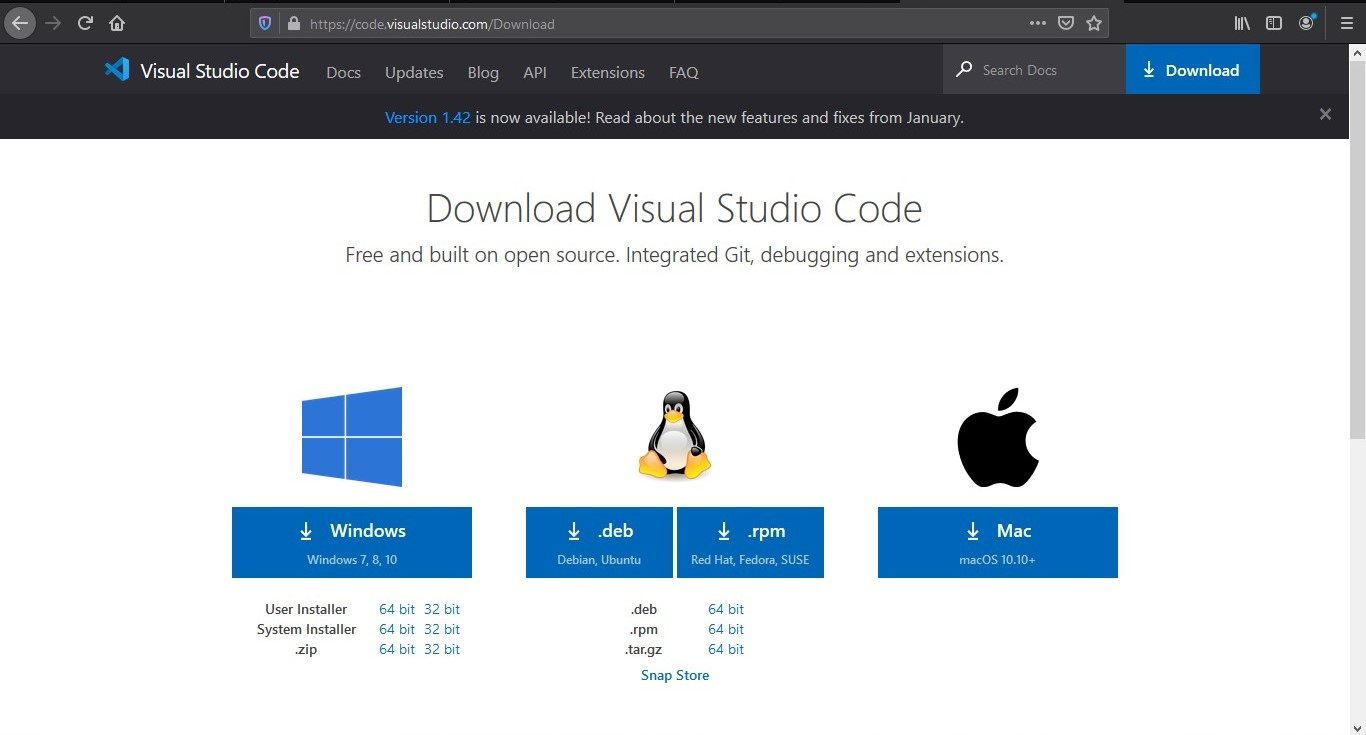
\includegraphics[scale=0.5]{Capitulo4/Documentos/imagenes_entorno/figura2-1-1.jpg}
    \caption{Ventana de descargas del editor Visual Studio Code, con el apartado .deb (paquete para equipos Linux basados en Debian) señalado.}
    \label{2.1.1}
\end{figure}

\noindent Una vez descargado el paquete se recurre a la instalación del .deb que es el requerido para la distribución que tengamos basada en Debian.  El gestor de paquetes de Ubuntu es el que controla la instalación, y para instalar Visual Studio Code se puede utilizar el centro de software de Ubuntu, el cual se muestra de manera automática cuando se hace doble clic sobre el paquete de instalación con extensión .deb. Este proceso identifica la aplicación que se desea instalar y muestra una interfaz al usuario en la que el mismo puede proceder a instalar la aplicación o a cancelar el proceso. La interfaz del centro de software de ubuntu muestra una pantalla como la de la figura \ref{2.1.2} cuando se hace doble clic sobre el paquete descargado previamente.

\begin{figure}[H]
    \centering
    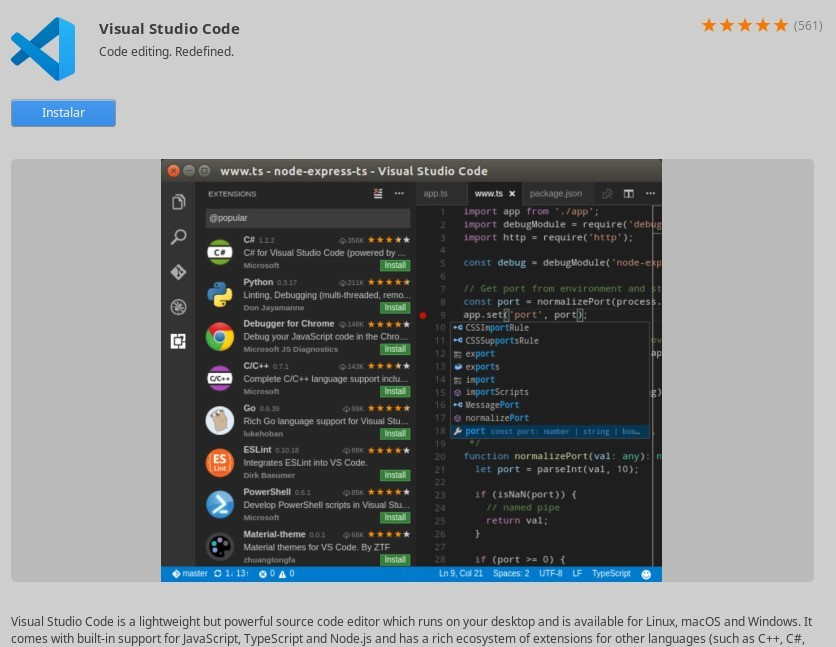
\includegraphics[scale=0.82]{Capitulo4/Documentos/imagenes_entorno/figura2-1-2.jpg}
    \caption{Instalación de Visual Studio Code mediante el centro de software de Ubuntu.}
    \label{2.1.2}
\end{figure}

\noindent Una vez concluida la instalación, para verificar que esta haya ido correctamente, se procede a abrir el editor, el cual debe mostrarse en una pantalla de inicio como la que ilustra la figura \ref{2.1.3}.

\begin{figure}[H]
    \centering
    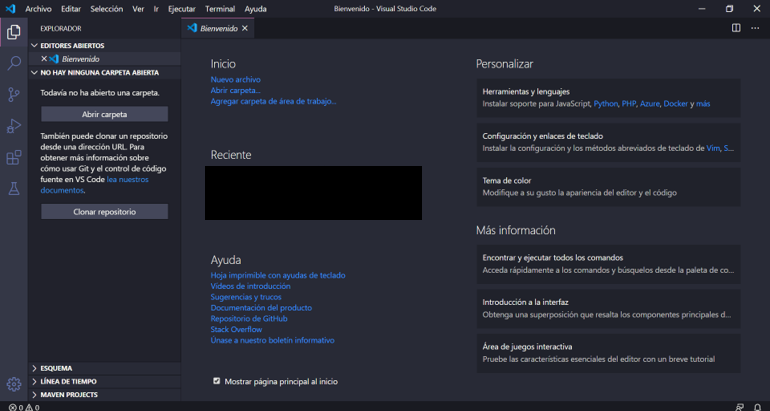
\includegraphics[scale=0.82]{Capitulo4/Documentos/imagenes_entorno/figura2-1-3.png}
    \caption{Ventana de inicio de Visual Studio Code.}
    \label{2.1.3}
\end{figure}

\subsubsection{Python en su versión 3}

\noindent El lenguaje con el que se desarrollará es Python, que para el caso de Ubuntu ya posee una versión de python instalada, para verificar esto se puede ingresar el siguiente comando en la terminal del sistema:
\begin{lstlisting}
python -V
\end{lstlisting}
La figura \ref{2.2.1} muestra el resultado de ejecutar este comando, el cual es el número de versión de python que el sistema tiene instalado en ese momento.

\begin{figure}[H]
    \centering
    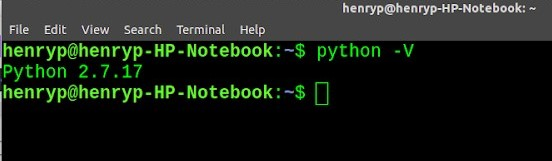
\includegraphics[scale=0.85]{Capitulo4/Documentos/imagenes_entorno/figura2-2-1.jpg}
    \caption{Resultado de la ejecución del comando para obtener la versión de python. En esta imagen se muestra que se tiene instalada la versión 2.7.}
    \label{2.2.1}
\end{figure}
\newpage
\noindent Sin embargo, para el desarrollo del sistema se requiere utilizar python en su versión 3.6.9. Para obtener esta versión en particular, se utiliza terminal para ingresar el siguiente comando:

\begin{lstlisting}
sudo add-apt-repository ppa:deadsnakes/ppa
sudo apt update
sudo apt install python3.6
\end{lstlisting}
\noindent Para corroborar la instalación de python en su versión 3.6.9, se ejecuta el comando:

\begin{lstlisting}
python3 -V
\end{lstlisting}
\noindent en la terminal del sistema. El resultado debe ser idéntico al que se puede ver señalado en la figura \ref{2.2.2}.
\begin{figure}[H]
    \centering
    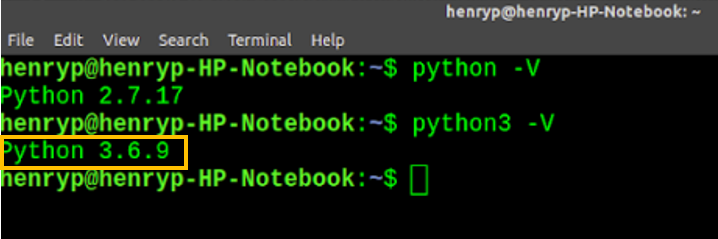
\includegraphics[scale=0.85]{Capitulo4/Documentos/imagenes_entorno/figura2-2-2.png}
    \caption{Verificación de la instalación de la versión correcta de python, se señala el resultado que indica la versión 3.6.9.}
    \label{2.2.2}
\end{figure}

\subsubsection{PIP}\\

\noindent PIP es un sistema de gestión de paquetes utilizado para instalar y administrar paquetes de software escritos en Python.\\

\noindent A partir de la instalación de python en la versión mayor a 3 (en este caso se utiliza la versión 3.6.9), PIP ya viene incluido (pero ahora es denominado PIP3), sin embargo, se puede verificar que ya se encuentra instalado ejecutando el siguiente comando en la terminal:

\begin{lstlisting}
pip3 --version
\end{lstlisting}

\noindent Como resultado de ejecutar este comando en la terminal se debe observar una respuesta del sistema similar a la que muestra la figura \ref{2.3.1}.

\begin{figure}[H]
    \centering
    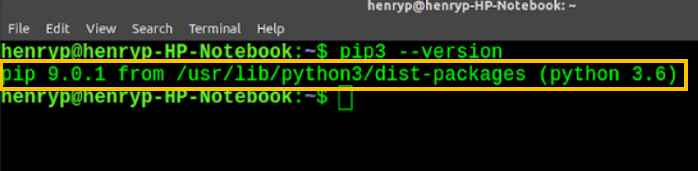
\includegraphics[scale=0.85]{Capitulo4/Documentos/imagenes_entorno/figura2-3-1.png}
    \caption{Comprobación de la instalación de PIP donde el resultado se encuentra señalado (incluso se indica para qué versión de python está configurado pip).}
    \label{2.3.1}
\end{figure}

\subsubsection{ChromeDriver}

\noindent Dado que se pretende trabajar con una biblioteca llamada Selenium, esta última requiere de un driver que sea compatible con el navegador deseado a trabajar, para el desarrollo del sistema de información, se optó por usar el navegador Google Chrome como el navegador predeterminado, para ello requerimos del driver de nombre ChromeDriver.\\

\noindent Antes de la descarga e instalación se deben de cumplir con algunos requisitos, y para instalar en ChromeDriver en el sistema operativo que se está utilizando, se debe empezar por lo ingresar los siguientes dos comandos en la terminal del sistema:
\begin{lstlisting}
sudo apt-get update
sudo apt-get install -z unzip xvfb libx16 libgconf 2-4
\end{lstlisting}

\noindent Posteriormente, se debe actualizar o instalar la versión más actual de Google Chrome, esto es más directo si se recurre a la página de descargas de Chrome, se descarga el .deb y se utiliza dicha herramienta de software para instalarlo.
La figura \ref{2.4.1} muestra la ventana de descargas del navegador. La misma página identifica el sistema operativo cuando se hace clic en el botón “Descargar Chrome”.

\begin{figure}[H]
    \centering
    
\includegraphics[scale=0.52]{Capitulo4/Documentos/imagenes_entorno/figura2-4-1.jpg}
    \caption{Página de descargas del navegador.}
    \label{2.4.1}
\end{figure}

Ya instalado el navegador, se puede continuar con el driver del navegador, para ello se visita la siguiente página:\\

\href{https://sites.google.com/a/chromium.org/chromedriver/downloads.}{https://sites.google.com/a/chromium.org/chromedriver/downloads.}\\

\noindent La figura \ref{2.4.2} ilustra una vista de la página de descargas descrita previamente.

\begin{figure}[H]
    \centering
    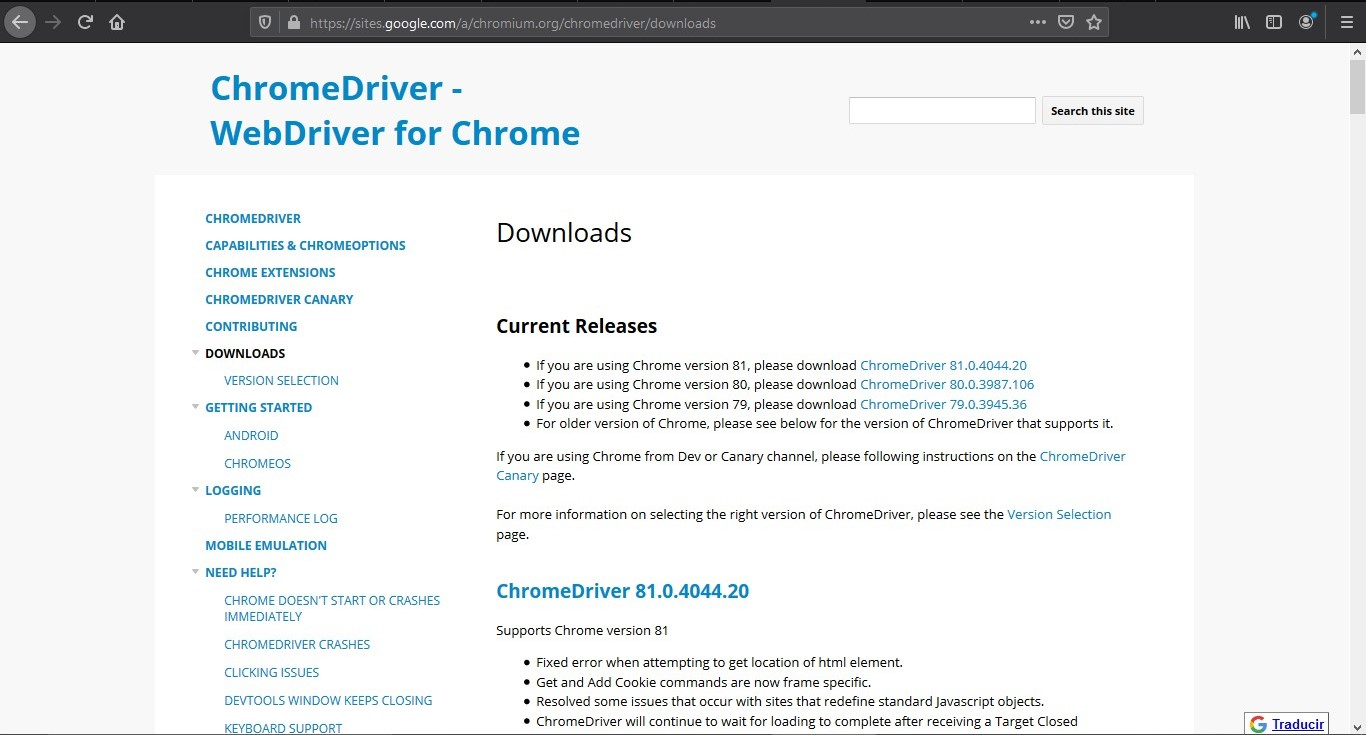
\includegraphics[scale=0.51]{Capitulo4/Documentos/imagenes_entorno/figura2-4-2.jpg}
    \caption{Página de descargas para el driver del navegador.}
    \label{2.4.2}
\end{figure}

\noindent Donde se selecciona el driver, según la versión del navegador Chrome que se tenga instalada, y se descarga el archivo. Ya con el archivo descargado, se obtiene su ubicación donde fue almacenado en el equipo y se hace clic derecho sobre el directorio seguido de la opción “Abrir en la terminal” para desplegar la pantalla de una terminal que ya esté directamente relacionada con la ruta donde se encuentra el archivo., una vez ahí, se ejecutan los siguientes comandos:

\begin{itemize}
    \item Se descomprime el .zip, cabe aclarar que se incluye en el comando, la característica del sistema, es decir los 64 bits.
\end{itemize}

\begin{lstlisting}
unzip chromedriver_linux64.zip  
\end{lstlisting}

\begin{itemize}
    \item Ya que se tiene el contenido, se realiza la instalación en el PATH:
\end{itemize}
\begin{lstlisting}
sudo mv chromedriver /usr/bin/chromedriver
sudo chown root:root /usr/bin/chromedirver
sudo chmod +x /usr/bin/chromedriver
\end{lstlisting}
\noindent Finalizado todo ya se cuenta con el driver necesario para la adquisición de los datos a través del navegador.
}
\\

\subsubsection{MGLTools}

\noindent MGLTools es un software desarrollado en el Laboratorio de Gráficos Moleculares (MGL) del Instituto de Investigación Scripps para la visualización y análisis de estructuras moleculares.
Utilizaremos esta herramienta para la transformación de las estructuras moleculares de los compuestos y las proteínas, esto  con la finalidad de generar receptores que puedan acoplarse a una estructura de un ligando.\\

\noindent Ejecutando la siguiente lista de comandos podremos descargar esta herramienta:
\begin{lstlisting}
wget http://mgltools.scripps.edu/downloads/downloads/tars
/releases/REL1.5.6/mgltools_x86_64Linux2_1.5.6.tar.gz
tar -xzvf mgltools_x86_64Linux2_1.5.6.tar.gz
cd mgltools_x86_64Linux2_1.5.6
./install.sh
cd MGLToolsPckgs/AutoDockTools/Utilities24
sudo cp prepare_ligand4.py /usr/local/bin
sudo cp prepare_receptor4.py /usr/local/bin
sudo cp prepare_gpf4.py /usr/local/bin
cd ../../..
cd bin
sudo cp pythonsh /usr/local/bin
\end{lstlisting}


\subsubsection{AutoDock-Vina}\\

\noindent AutoDock Vina es un conjunto de herramientas de acoplamiento automatizadas. Está diseñado para predecir cómo las moléculas pequeñas, como sustratos o candidatos a fármacos, se unen a un receptor de estructura 3D conocida.\\

\noindent Esta herramienta sera utilizada para realizar un docking más preciso introduciendo las estructuras del ligando y el receptor.
Para realizar su instalación ejecutaremos la siguiente lista de comandos:
\begin{lstlisting}
sudo wget http://vina.scripps.edu/download/autodock_vina_1_1_2_linux_x86.tgz
echo descomprimir
tar -xzvf autodock_vina_1_1_2_linux_x86.tgz
cd autodock_vina_1_1_2_linux_x86/bin
cp vina /usr/local/bin
\end{lstlisting}

\subsubsection{AutoGrid}\\

\noindent AutoGrid es un programa que calcula previamente los mapas de cuadrícula de las energías de interacción para varios tipos de átomos, como los carbonos alifáticos, los carbonos aromáticos, los oxígenos de enlace de hidrógeno, etc., con una macromolécula como una proteína, ADN o ARN.\\

\noindent Estos mapas de cuadrícula se utilizan luego en los cálculos de acoplamiento de AutoDock para determinar la energía de interacción total para un ligando con una macromolécula.

\noindent Para la instalación de esta herramienta, ejecutamos la siguiente lista de comandos en la terminal:
\begin{lstlisting}
sudo wget http://autodock.scripps.edu/downloads/
autodock-registration/tars/dist426/
autodocksuite-4.2.6-x86_64Linux3.tar
echo Descomprimiendo autodocksuite
tar -xvf autodocksuite-4.2.6-x86_64Linux3.tar
cd x86_64Linux3
cp autodock4 /usr/local/bin
cp autogrid4 /usr/local/bin
\end{lstlisting}
\subsection{Bibliotecas}{
\noindent La instalación de bibliotecas se realiza utilizando el administrador de paquetes para python PIP en su versión para python3 el cual corresponde al comando de pip3, cuya instalación se menciona en el apartado X. Es importante señalar que para todas las bibliotecas que se van a instalar se requiere conexión a internet. Para verificar la correcta instalación de cada biblioteca, basta con dar seguimiento a la información que el sistema va mostrando mientras se encuentra instalando la biblioteca especificada. Las bibliotecas aquí descritas cuando han sido correctamente instaladas muestran un mensaje (definido por pip3) como el que se señala en la figura \ref{3.1}, donde se toma como ejemplo la instalación de la biblioteca Requests, y al final puede leerse la frase en inglés “Successfully installed” seguido del nombre completo de la biblioteca.

\begin{figure}[H]
    \centering
    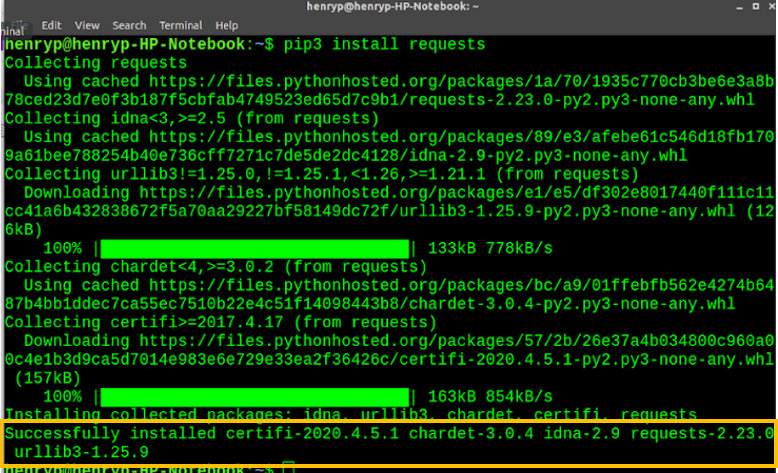
\includegraphics[scale=0.85]{Capitulo4/Documentos/imagenes_entorno/figura3-1.png}
    \caption{Instalación exitosa de la biblioteca Requests, donde se señala el mensaje que arroja pip3 de éxito del proceso de instalación.}
    \label{3.1}
\end{figure}
\subsubsection{Tkinter}\\

\noindent Con Python hay muchas posibilidades para programar una interfaz gráfica de usuario (GUI) pero Tkinter es fácil de usar, es multiplataforma y, además, viene incluido con Python en su versión para Windows, para Mac y para la mayoría de las distribuciones GNU/Linux. Se le considera el estándar de facto en la programación GUI con Python.\\

\noindent Tkinter es un binding de la biblioteca Tcl/Tk que está también disponible para otros lenguajes como Perl y Ruby.
A pesar de su larga historia, su uso no está demasiado extendido entre los usuarios de equipos personales porque su integración visual con los sistemas operativos no era buena y proporcionaba pocos widgets (controles) para construir los programas gráficos.
Para instalar Tkinter se debe escribir y ejecutar el siguiente comando en la terminal:
\begin{lstlisting}
sudo apt-get install python3-tk
\end{lstlisting}
\noindent Para verificar esta instalación, se procede a ingresar a la línea de comandos de python3 simplemente ejecutando en la terminal el comando:
\begin{lstlisting}
python3 
\end{lstlisting}
\noindent Luego se procede a escribir las siguientes dos líneas:
\begin{lstlisting}
import tkinter
tkinter.TkVersion
\end{lstlisting}
\noindent Si la instalación se ha hecho correctamente, la terminal arroja un resultado como el que se señala en la figura \ref{3.1.1}.

\begin{figure}[H]
    \centering
    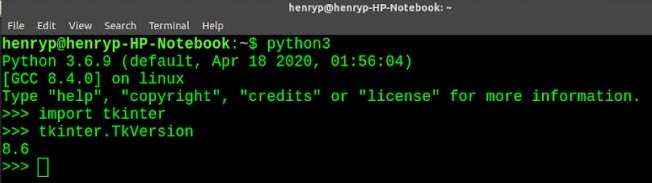
\includegraphics[scale=0.85]{Capitulo4/Documentos/imagenes_entorno/figura3-1-1.jpg}
    \caption{Confirmación de la instalación de Tkinter.}
    \label{3.1.1}
\end{figure}
\subsubsection{Requests}\\

\noindent Requests es una librería de Python para peticiones HTTP liberada bajo una la licencia de Apache License 2.0.  Request permite enviar solicitudes HTTP / 1.1 con extrema facilidad.\\ 

\noindent No es necesario agregar manualmente cadenas de consulta a sus URL, ni codificar de forma estricta los datos POST. Keep-alive y el grupo de conexiones HTTP son 100\% automáticas.\\

\noindent La instalación en Linux es de la siguiente manera. Como ya se ha instalado PIP en la versión para python3, basta con el siguiente comando:\\

\begin{lstlisting}
pip3 install requests
\end{lstlisting}

\subsubsection{Selenium}\\

\noindent Selenium para Python proporcionan una API simple para navegar o realizar pruebas en algún navegador web, utilizando un WebDriver. A través de Selenium Python API puede acceder a todas las funcionalidades de Selenium WebDriver de una manera sencilla e intuitiva.\\
Selenium Python proporcionan una API conveniente para acceder a Selenium WebDrivers como Firefox, Internet Explorer, Chrome, Remote, etc. Y es compatible con versiones de Python desde la 2.7.\\

\noindent
Para la instalación se ejecuta el siguiente comando en la terminal del sistema:
\begin{lstlisting}
pip3 install selenium
\end{lstlisting}

\subsubsection{Pillow}\\

\noindent Es una librería gratuita que permite la edición de imágenes directamente desde Python. Soporta una variedad de formatos, incluidos los más utilizados como GIF, JPEG y PNG. Una gran parte del código está escrito en C, por cuestiones de rendimiento.\\

\noindent Debido a que la librería soporta únicamente hasta la versión 2.7 de Python y, al parecer, no se propuso avanzar con él, un equipo de desarrolladores en colaboración se ha desarrollado Pillow, una bifurcación, con un desarrollo más «amigable», así nace PIL que pretende mantener una librería estable y que se adapte a las nuevas tecnologías (De Python 3 en adelante). Por esta razón, PIL entró en función en lugar de Pillow.\\

\noindent Para proceder con la instalación, se ingresa y ejecuta el siguiente comando en la terminal del sistema:

\begin{lstlisting}
pip3 install Pillow
\end{lstlisting}

\subsubsection{BioPython}

\noindent BioPython es el nombre que recibe una serie de aplicaciones y programas informáticos pensados para cuantificar y hacer cálculos con datos biológicos, programados por una comunidad internacional. El uso de esta biblioteca apoya en aportar el mayor número posible de bibliotecas informáticas basadas en el lenguaje de programación Python, que usualmente para tener aplicaciones bioinformáticas y que estén disponibles para un público lo más amplio posible.\\

\noindent Se hace uso de BioPython ya que   permite representar secuencias biológicas y anotaciones de genomas y es capaz de comunicar con las bases de datos biológicos en línea del NCBI para hacer cálculos. Además, gracias a diversos módulos, puede ser utilizada para trabajar sobre proyectos relativos al alineamiento de secuencias, cálculo de estructuras proteicas, genética de poblaciones, filogenética e inteligencia artificial.\\

\noindent Para instalarlo, se puede realizar a través de los comandos, cabe mencionar que las versiones recientes de Python (comenzando con Python 2.7.9 y Python 3.4) incluyen la herramienta de administración de paquetes Python, que permite una instalación fácil desde la línea de comandos en todas las plataformas:
\begin{lstlisting}
pip3 install biopython
\end{lstlisting}

\subsubsection{PubChemPy}\\

\noindent La biblioteca PubChemPy proporciona una forma de interactuar con la base de datos PubChem en Python. Permite búsquedas químicas por nombre, subestructura y similitud, estandarización química, conversión entre formatos de archivos químicos, representación y recuperación de propiedades químicas.\\
 
\noindent Para la instalación se procede a ejecutar el siguiente comando en la terminal del sistema:
\begin{lstlisting}
pip3 install pubchempy
\end{lstlisting}
\noindent Esencialmente esta biblioteca consta de realizar solicitudes a servidores de esta plataforma, dicha solicitud se evalúa y luego se envía una respuesta. Sin embargo pueden haber algunos inconvenientes, se requiere una conexión constante a Internet y algunas tareas serán más lentas que si se realizan localmente en una propia computadora. Por lo que estos requerimientos, se deben de contemplar al codificar.

\subsubsection{Pypdb}

\noindent Una interfaz de programación Python para el Banco de datos de proteínas RCSB (PDB) que permite la búsqueda y recuperación de datos para una amplia gama de tipos de resultados, incluidas BLAST y consultas de secuencias.\\

\noindent La API se auxilia de XML existente y funciona creando solicitudes personalizadas a partir de tipos nativos de Python, lo que permite la extensibilidad y la modificación directa. La librería tiene la capacidad de realizar muchos tipos de búsqueda avanzada del Banco de datos de proteínas que, de lo contrario, solo están disponibles a través del sitio web de PDB.\\

Basta con ejecutar el siguiente comando en la terminal del sistema:
\begin{lstlisting}
pip3 install pypdb
\end{lstlisting}

\subsubsection{Ratelimit}

\noindent Las API son una forma muy común de interactuar con los servicios web. A medida que crece la necesidad de consumir datos, también lo hace la cantidad de llamadas API necesarias para mantenerse actualizado con las fuentes de datos. Sin embargo, muchos proveedores de API impiden que los desarrolladores realicen demasiadas llamadas a la API. Esto se conoce como limitación de velocidad y, en el peor de los casos, se puede prohibir que su aplicación realice más llamadas API si abusa de estos límites.\\

\noindent Este paquete presenta un decorador de funciones que evita que una función se llame con más frecuencia que la permitida por el proveedor de API. Esto debería evitar que los proveedores de API prohíban sus aplicaciones conforme a sus límites de velocidad.\\

\noindent Utilizando el siguiente comando en la terminal se instala la biblioteca ratelimit:

\begin{lstlisting}
pip3 install ratelimit
\end{lstlisting}
}
\\
\subsubsection{Pandas}

\noindent Pandas es un paquete de Python de código abierto que proporciona numerosas herramientas para el análisis de datos. El paquete viene con varias estructuras de datos que se pueden usar para muchas tareas diferentes de manipulación de datos. También tiene una variedad de métodos que se pueden invocar para el análisis de datos, lo cual es útil cuando se trabaja en ciencia de datos y problemas de aprendizaje automático en Python.\\

Para realizar la instalación de esta biblioteca, se ejecuta el siguiente comando en la terminal:\\

\begin{lstlisting}
pip3 install pandas
\end{lstlisting}

\subsubsection{Scikit-learn}

\noindent Scikit-learn proporciona una gama de algoritmos de aprendizaje supervisados ​​y no supervisados ​​a través de una interfaz consistente en Python.
Se licencia bajo una licencia BSD simplificada permisiva y se distribuye bajo muchas distribuciones de Linux, fomentando el uso académico y comercial.
La biblioteca está construida sobre SciPy (Scientific Python) que debe instalarse antes de poder usar scikit-learn. Esta pila que incluye:

\begin{itemize}
    \item NumPy: paquete de matriz base n-dimensional
    \item SciPy: biblioteca fundamental para la computación científica
    \item Matplotlib: trazado 2D / 3D completo
    \item IPython: consola interactiva mejorada
    \item Sympy: matemática simbólica
    \item Pandas: estructuras de datos y análisis
\end{itemize}

\noindent Las extensiones o módulos para SciPy se denominan convencionalmente SciKits. Como tal, el módulo proporciona algoritmos de aprendizaje y se llama scikit-learn.
La visión de la biblioteca es un nivel de robustez y soporte requerido para su uso en sistemas de producción. Esto significa un enfoque profundo en preocupaciones tales como la facilidad de uso, la calidad del código, la colaboración, la documentación y el rendimiento.\\

\noindent Para instalar el paquete de bibliotecas de scikit-learn se ejecuta en la terminal del equipo el siguiente comando:

\begin{lstlisting}
pip3 install scikit-learn
\end{lstlisting}

\subsubsection{NumPy}{
\noindent NumPy es el paquete fundamental para la computación científica en Python. Es una biblioteca de Python que proporciona un objeto de matriz multidimensional, varios objetos derivados (como matrices y matrices enmascaradas), y una variedad de rutinas para operaciones rápidas en matrices, que incluyen matemática, lógica, manipulación de formas, clasificación, selección, E / S , transformadas discretas de Fourier, álgebra lineal básica, operaciones estadísticas básicas, simulación aleatoria y mucho más.\\

Para instalar esta biblioteca se ejecuta en la terminal del equipo el siguiente comando:

\begin{lstlisting}
pip3 install numpy
\end{lstlisting}
}
}
%% ------------------- Generación del Código de los Componentes y Procedimientos --------------------------------------- %%
\section{Generación del Código de los Componentes y Procedimientos}
 \noindent Este documento describe el diseño de la lógica de programación y los algoritmos utilizados para la solución de los diversos problemas que implicaba la generación del código de los componentes de SisPAF.\\
 
 \noindent SisPAF es un sistema compuesto por 3 módulos principales, cada uno contando con su propio desarrollo para la interfaz y para el código que acompaña dicha interfaz. La figura X ilustra el modelo lógico del sistema donde se pueden observar los 3 módulos antes mencionados, los cuales son:\\
 
 \subsubsection{Búsqueda de información:}\label{Busqueda}
 \noindent El módulo de búsqueda de información es el primer módulo de SisPAF y es el encargado de obtener la información necesaria para realizar la predicción de la actividad farmacológica (efectividad de los fármacos frente a cierta patología).\\
 
 \subsubsection{Análisis de la información:}
\noindent Una vez obtenidos los datos del módulo de búsqueda y que el usuario es informado de los resultados de dicha búsqueda, se procede a realizar un análisis de la información obtenida. Para esto se empleo el uso de un método de la bioinformática conocido como modelo QSAR (por sus siglas en inglés, \textit{Quantitative Structure Activity Relationship}) que permite relacionar a los compuestos con determinadas proteínas y predecir qué tan efectivos pueden ser para atacar y destruir esas proteínas. Dentro del mismo modelo QSAR se utilizan algoritmos de \textit{Machine Learning}, en este caso regresión lineal múltiple y mapa auto-organizado para generar los resultados que representan la efectividad de los compuestos, previamente mencionada.

\subsubsection{Generación de resultados:}
\noindent En este módulo, los resultados del análisis son ordenados y desplegados al usuario en una interfaz, para su visualización con opción a ser almacenados en el sistema.

\begin{figure}[H]
    \centering
    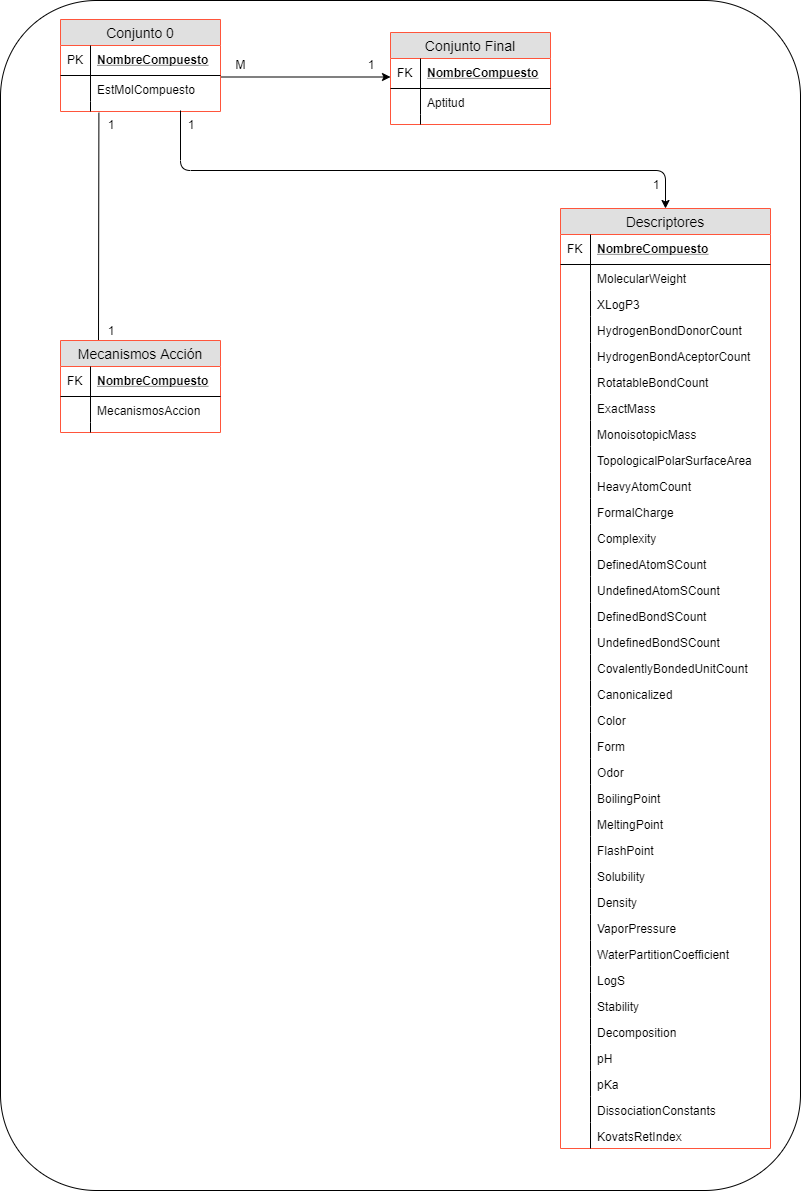
\includegraphics[scale=0.40]{Capitulo4/Documentos/imagenes_generacion/modeloDatosLogico.png}
    \caption{Modelo lógico de SisPAF.}
    \label{Modelo_logico_de_SisPAF_1}
\end{figure}

\subsubsection{Generación de código de los componentes}
\subsection{Búsqueda de información}
\noindent Este módulo incluye desde la ventana de inicio de SisPAF (descrita en el apartado \ref{Busqueda}) hasta la confirmación de los resultados de la búsqueda. El usuario ingresa un archivo inicial (véase en la tabla \ref{diccionario}) o indica un directorio donde se encuentre un proyecto ya existente.  SisPAF analiza ya sea el directorio o el archivo inicial y recopila información sobre los compuestos y proteínas de los que se desean obtener datos en específico (estructura molecular de los compuestos, estructura molecular de las proteínas, descriptores físico químicos de los compuestos, mecanismos de acción de los compuestos). Cuando SisPAF determina los elementos (compuestos y proteínas indicados por el usuario) de los cuales debe obtener dichos datos, realiza las conexiones correspondientes con las bases de datos en línea que proveen esa información (en la figura \ref{DFD1} se observan las 3 bases de datos, DrugBank, PDB,  PubChem, y la información que de ellas se obtiene). Finalmente se despliega al usuario una tabla con un resumen de qué datos se obtuvieron para cada uno de los elementos identificados.\\

\noindent El diagrama de flujo que ilustra la figura \ref{DFD1}. muestra las actividades que componen al módulo de búsqueda de información, las cuales de describen a continuación.

\begin{figure}[H]
    \centering
    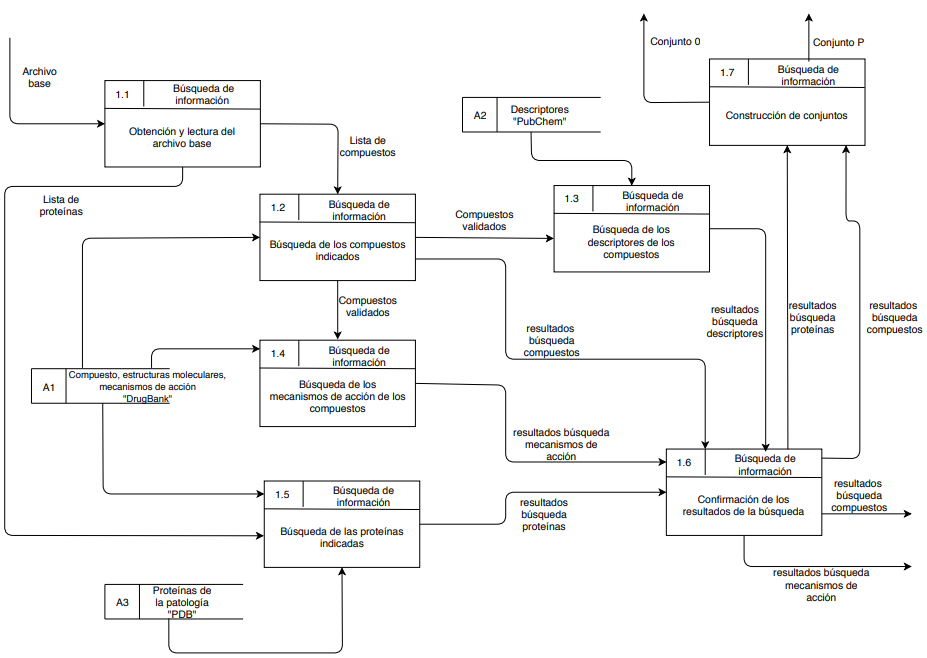
\includegraphics[scale=0.46]{Capitulo2/images/DFD-1.png}
    \caption{Diagrama de flujo de datos del módulo de búsqueda de información.}
    \label{DFD1}
\end{figure}
%%%%%%%%%%%%%%%%%%%%%%%%%%%%%%%%%%%%%%%%%%%%%%%%%%%%%%%%%%%%%%%
\subsubsection{Diseño de interfaces}{
\noindent Al momento de  realizar el análisis y diseño del sistema de información,  se plantearon las vistas que tendrían las interfaces, empezando por las que comunican al usuario con las funciones más importantes del sistema, como la adquisición del archivo inicial, si existe un  error en este, entre otras interacciones importantes al iniciar SisPAF.\\

\noindent A continuación mostramos las pantallas que se consideran importantes, y el resultado al ser programadas en el lenguaje Python, auxiliándose en la librería Tkinter.

\begin{figure}[H]
    \centering
    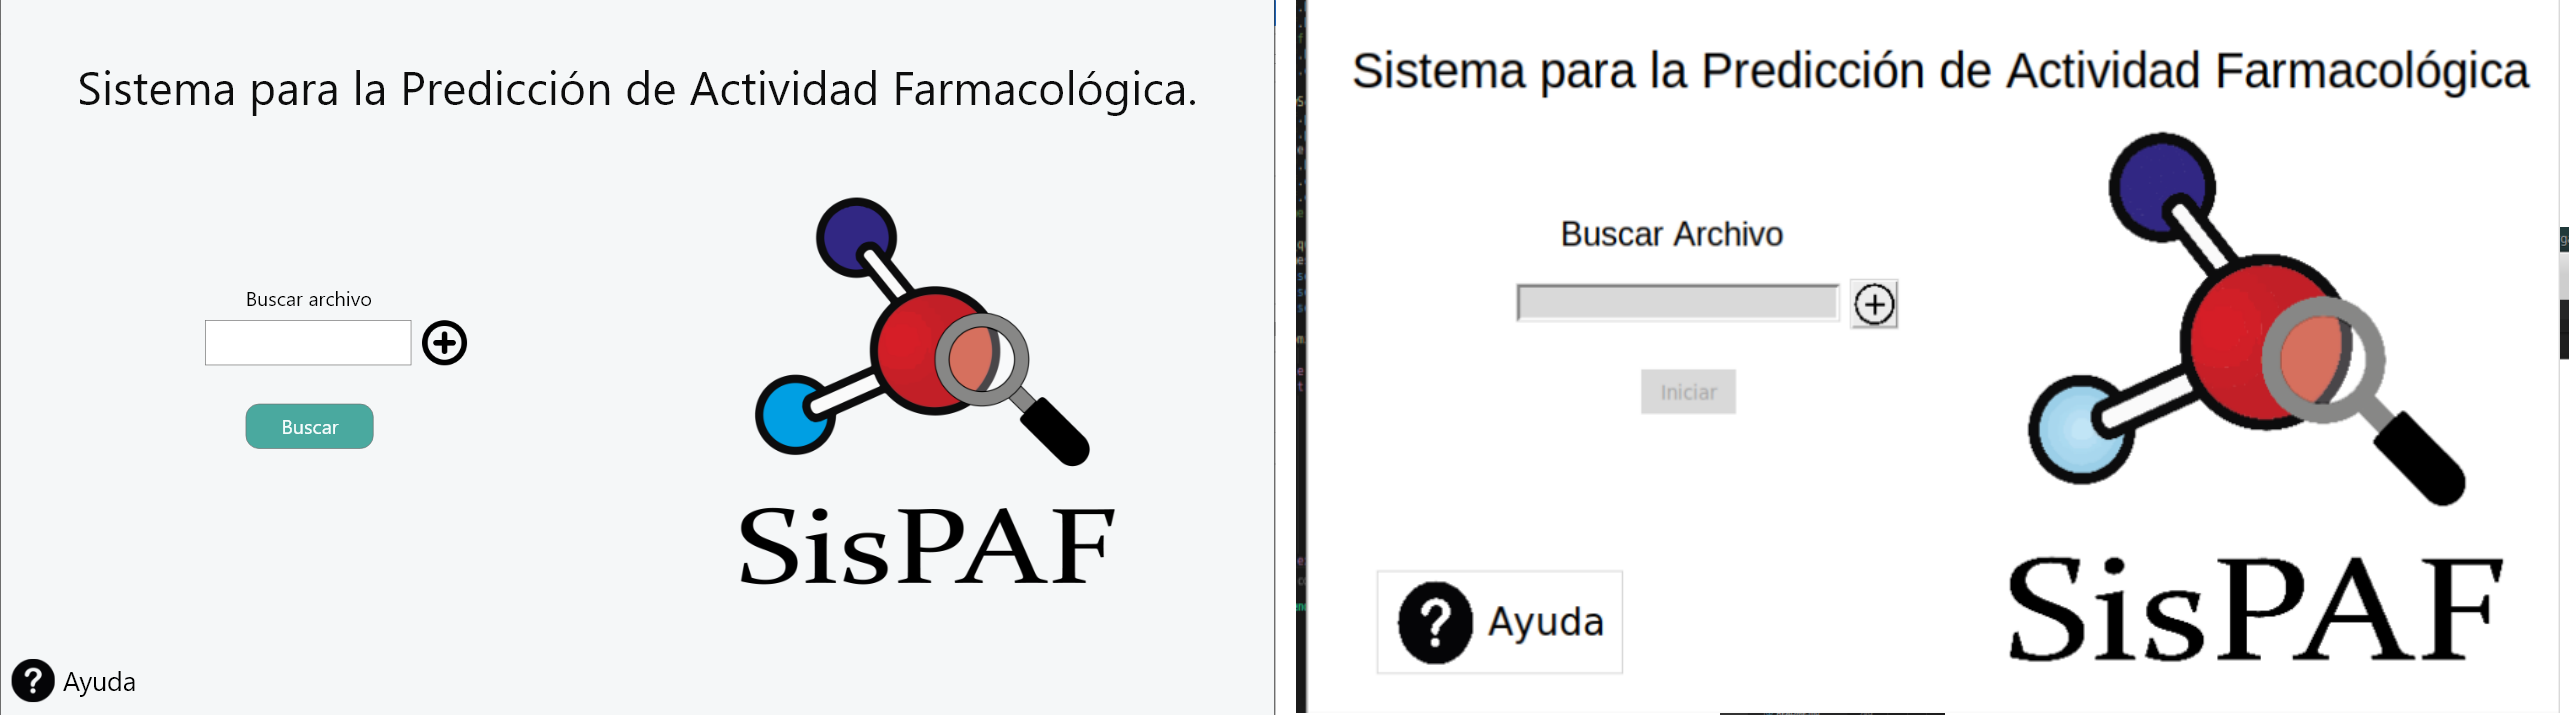
\includegraphics[scale=0.215]{Capitulo4/Documentos/imagenes_generacion/ComparacionPan1.png}
    \caption{Comparación de pantallas, a la izquierda la diseñada y  a la derecha la pantalla programada.}
    \label{comparacion}
\end{figure}

\noindent A esas pantallas se han incluido mensajes de error, que igual estaban planificados para cuando existieran posibles fallos, uno de ellos, es cuando el archivo no contiene el formato y/o contenido adecuado.\\

\begin{figure}[H]
    \centering
    
\includegraphics[scale=0.375]{Capitulo4/Documentos/imagenes_generacion/PickwrongAr.png}
    \caption{Comparación de mensajes de error, a la izquierda la planeada y a la derecha la programada.}
    \label{comparacion_2}
\end{figure}

}
%%%%%%%%%%%%%%%%%%%%%%%%%%%%%%%%%%%%%%%%%%%%%%%%%%%%%%%%%%%%%%
\subsubsection{Inicio}{
\noindent La interfaz de inicio funciona como una especie de canalizador. Dependiendo de si el usuario quiere crear un nuevo proyecto o abrir uno ya existente, los procesos a ejecutar son diferentes hasta que se llega a la parte del análisis de información. Para comenzar, cualquier botón solicita al usuario que seleccione un directorio (para crear o para abrir un proyecto). Si se desea crear un nuevo proyecto se procede a mostrar la interfaz correspondiente que le permite al usuario cargar al sistema un archivo inicial y comenzar con el proceso de la búsqueda de información. Por otro lado si el usuario elige abrir un proyecto el sistema solicita que se le indique el directorio donde se encuentra dicho proyecto y procede a analizar la estructura del directorio para definir la información que ya se ha obtenido y continuar el proceso desde el punto necesario.\\
}
%%%%%%%%%%%%%%%%%%%%%%%%%%%%%%%%%%%%%%%%%%%
\subsubsection{Obtención y lectura del archivo inicial}{
\noindent El proceso para realizar la obtención y la lectura del archivo inicial (véase \ref{diccionario}) involucra la comunicación de la interfaz que es la que determina dónde se va a almacenar dicho archivo y el uso de herramientas básicas de lectura y escritura presentes en python. Python permite abrir un archivo simplemente con especificar la ruta donde se encuentra almacenado. Luego se realiza la lectura del archivo mediante un ciclo que lee línea por línea hasta que se encuentra con el final de dicho archivo. Durante esta lectura es donde es posible almacenar la información requerida en dos secciones separadas, en este caso una sección para compuestos y una para proteínas. Estos dos apartados definen los elementos cuya información debe ser buscada en la base de datos en línea.
En este proceso se hace presente la comprobación de la estructura del archivo inicial, la cual es representada de manera gráfica por la figura \ref{flujo}.\\


\noindent La figura \ref{flujo} contiene el diagrama de flujo para el proceso de comprobación del archivo inicial, el cual se basa en revisar la presencia de las etiquetas (Compounds y Proteins) y enviar una alerta al usuario en caso de que no se encuentren dichas etiquetas. El mismo SisPAF, al momento de leer y almacenar la información del archivo inicial, es capaz de detectar elementos duplicados, haciendo que los elementos obtenidos sean únicos.

\begin{figure}[H]
    \centering
    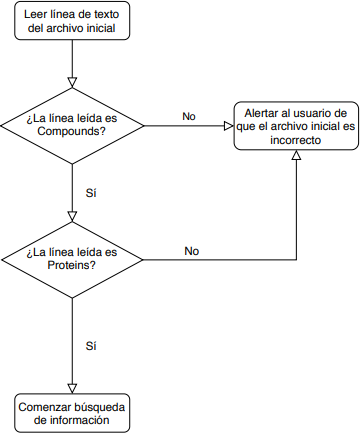
\includegraphics[scale=0.85]{Capitulo4/imagenes/diagramaArchivoInicia.png}
    \caption{Diagrama de flujo del análisis del archivo inicial.}
    \label{flujo}
\end{figure}
}
%%%%%%%%%%%%%%%%%%%%%%%%%%%%%%%%%%%%%%%%%%%%%%%%%%%%%
\subsubsection{Diseño de interfaces}{
\noindent Para el módulo de la búsqueda de datos, se diseñaron interfaces que muestran el status del sistema durante la conexión a las bases de datos, mostrar el resultado de dichas consultas, dándole a saber al usuario si hubo un error en la adquisición de la información necesario de los compuestos o las proteínas.\\

\noindent A continuación se muestra la pantalla de espera, mientras el sistema realiza la búsqueda de información, con la cual se le indica al usuario que el sistema sigue trabajando.
}

\begin{figure}[H]
    \centering
    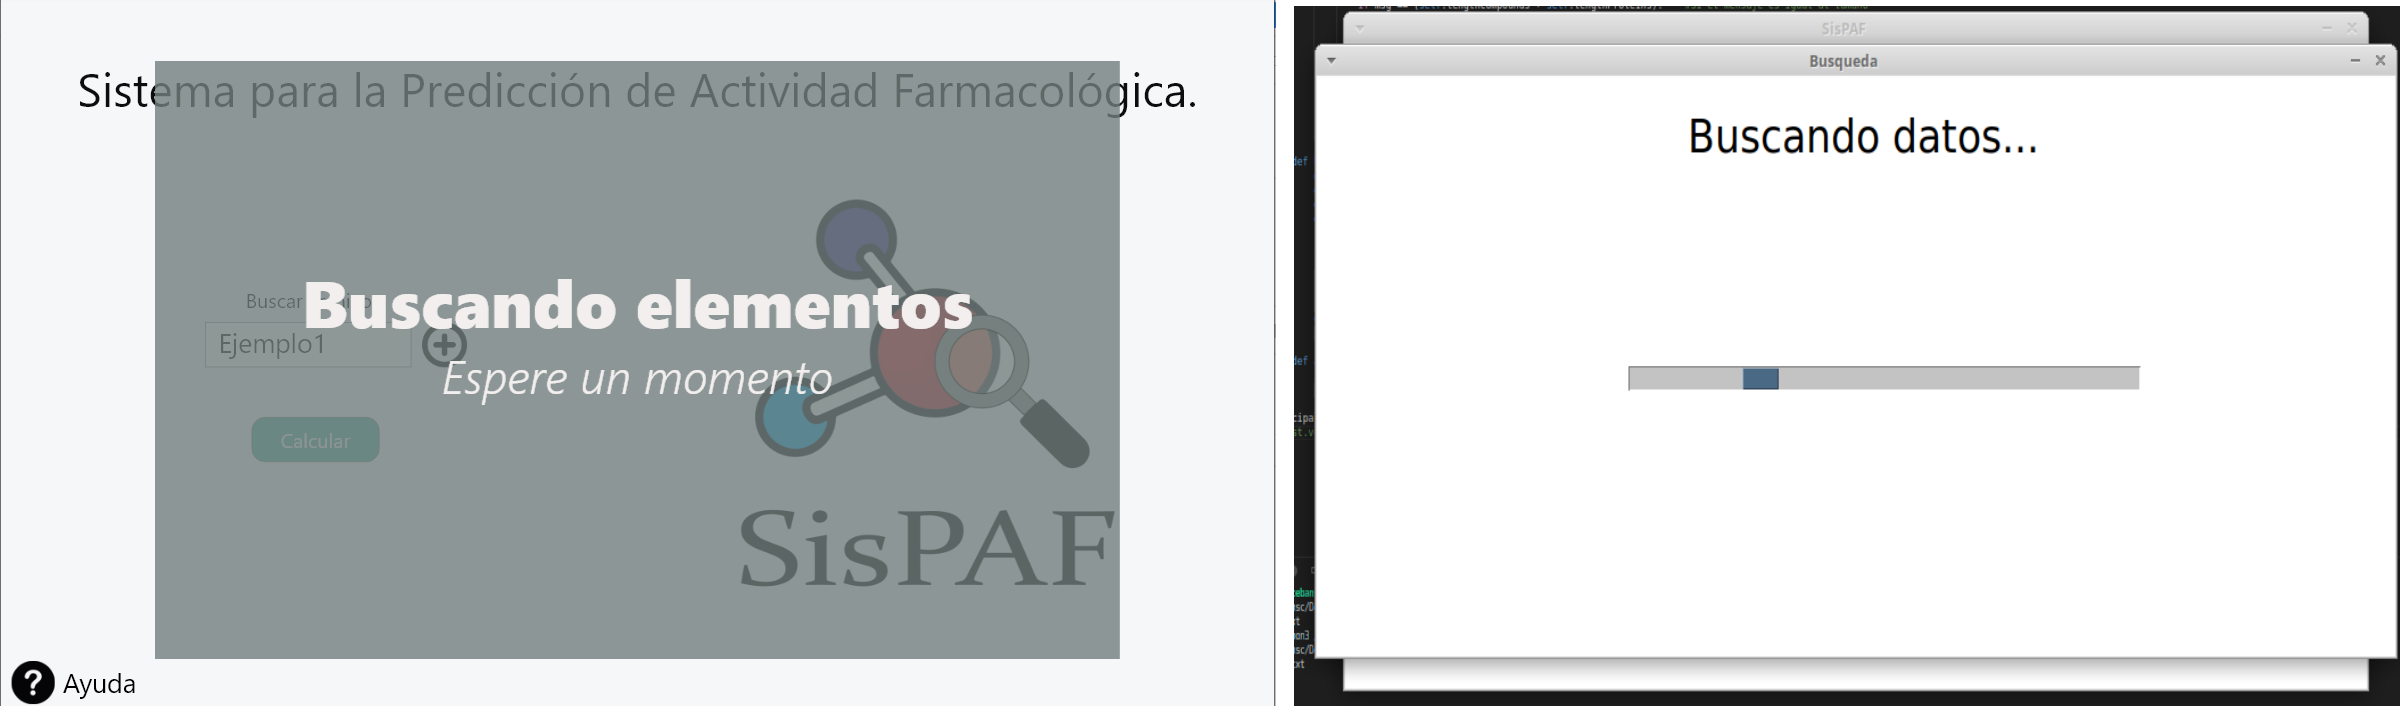
\includegraphics[scale=0.235]{Capitulo4/Documentos/imagenes_generacion/Esperabusqueda.png}
    \caption{Comparación de pantallas de espera para la búsqueda de información, a la izquierda la planeada y a la derecha la programada.}
    \label{comparacion_3}
\end{figure}

\noindent Durante la búsqueda, el mayor problema, incluso considerarse fatal, sería la pérdida de conexión a internet, para ello se planeó en un inicio la aparición de un mensaje de error para cuando esto suceda.

\begin{figure}[H]
    \centering
    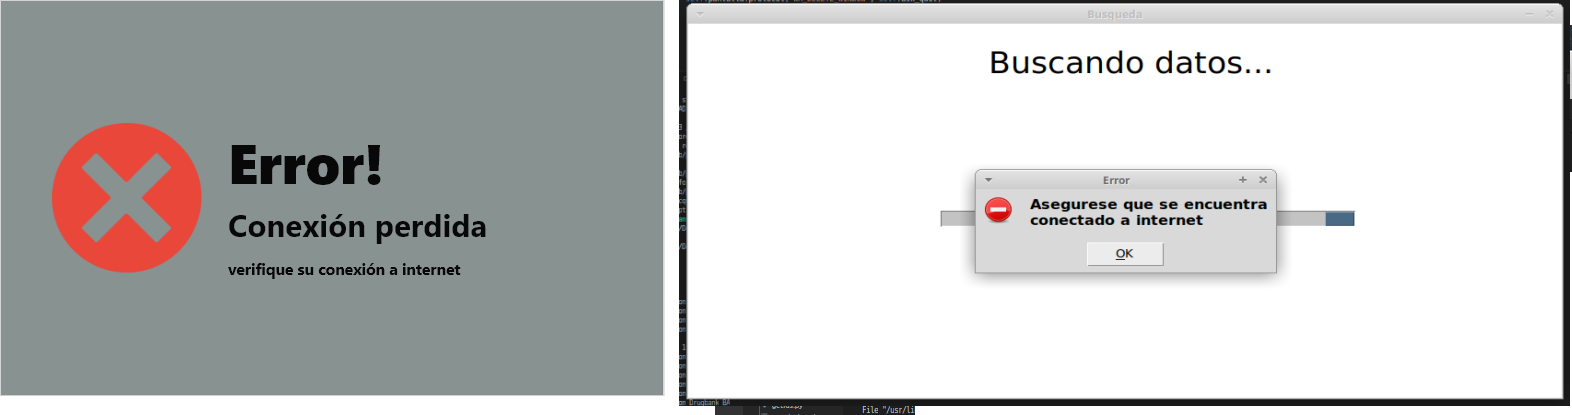
\includegraphics[scale=0.375]{Capitulo4/Documentos/imagenes_generacion/errorNet.png}
    \caption{Comparación de mensajes de error en la pérdida de conexión, a la izquierda la planeada y a la derecha la programada.}
    \label{comparacion_4}
\end{figure}

\noindent Cuando la búsqueda de datos, ha finalizado, al usuarios se muestra una pantalla que indica el estado de cada compuesto y proteína respecto a la información que nos interesa de ellos, si no se encontró la estructura del compuesto, o de la proteína, etc.

\begin{figure}[H]
    \centering
    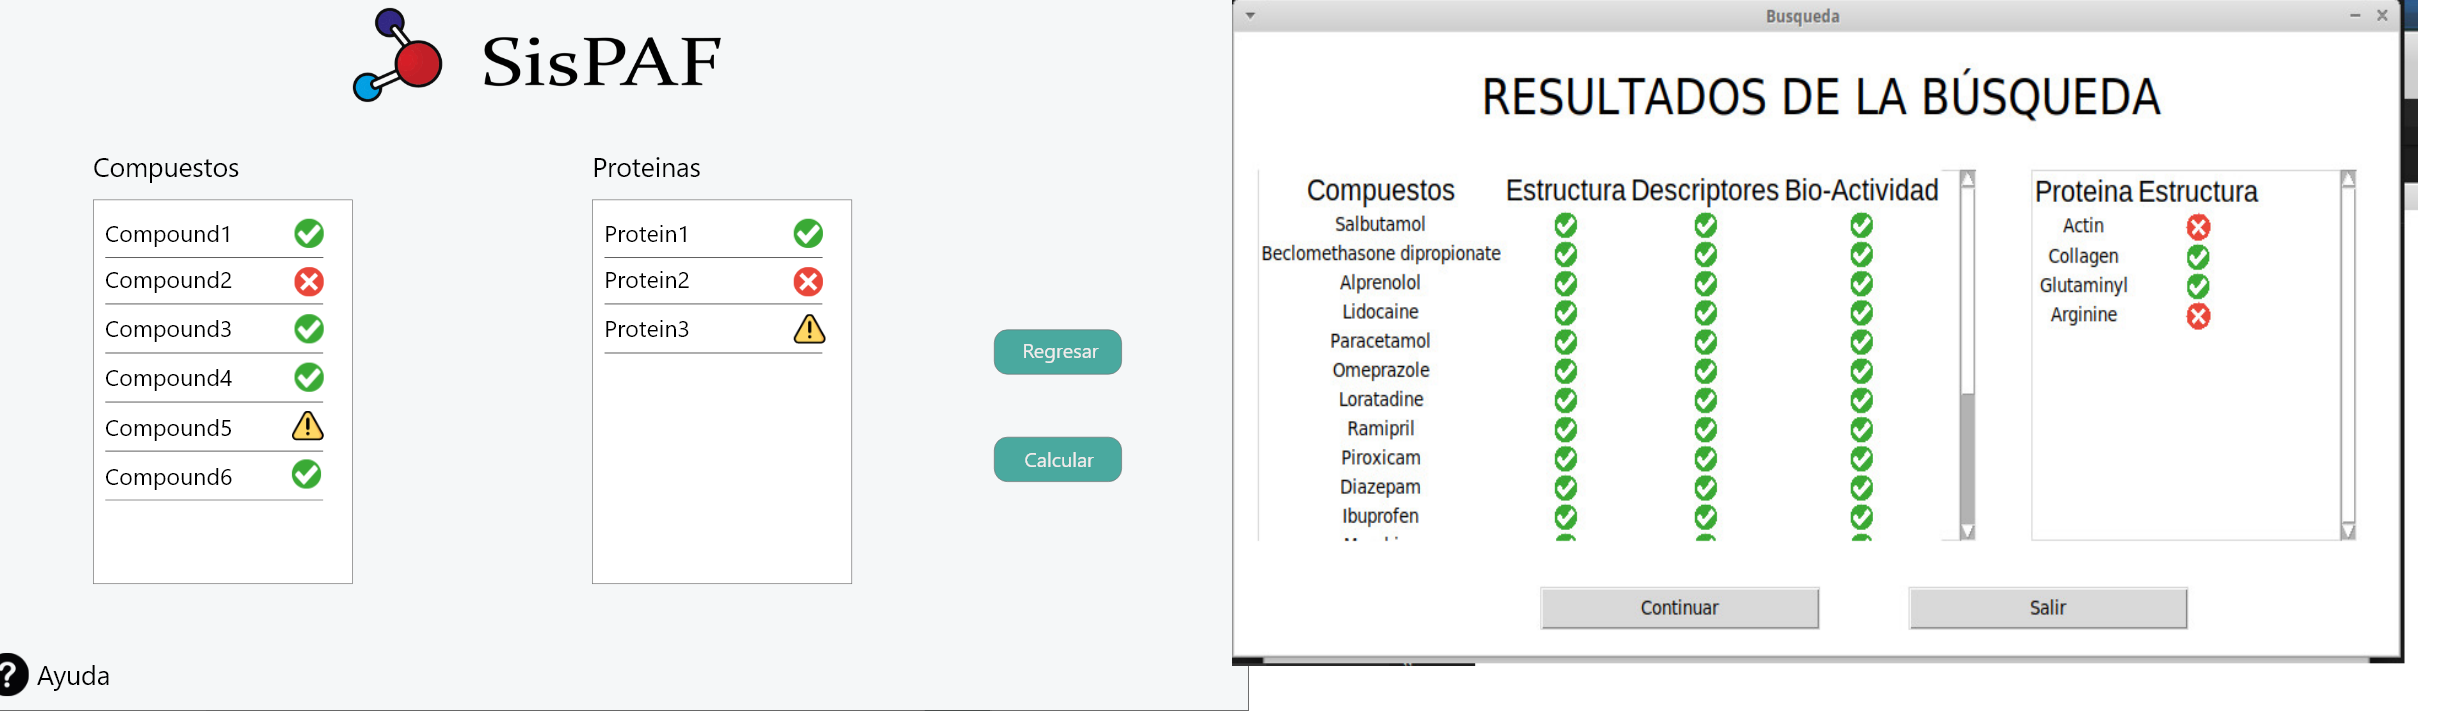
\includegraphics[scale=0.225]{Capitulo4/Documentos/imagenes_generacion/ResultBusqueda.png}
    \caption{Comparación de pantallas para resultados de búsqueda, a la izquierda la planeada y a la derecha la programada.}
    \label{comparacion_5}
\end{figure}
%%%%%%%%%%%%%%%%%%%%%%%%%%%%%%%%%%%%%%%%%%%%%%%%%%%%%%%%%%%%%%
\subsubsection{Búsqueda de información: uso de API’s y Web scrapping}
\noindent Cuando ya se han definido los elementos de los cuales se debe obtener su información, se procede a utilizar API’s que las bases de datos en línea poseen y que utilizan para consultar la información de dichas bases de datos. Para realizar las llamadas a las API se deben tomar en cuenta dos cosas: la cantidad límite de peticiones por segundo que cada API define para evitar saturarse de solicitudes y la manera en cómo debe accederse a la información que se requiere obtener (para este caso, la estructura molecular, los descriptores fisicoquímicos computados y los mecanismos de acción para cada uno de los  compuestos, mientras que para las proteínas solo se requiere la estructura molecular).

\noindent En esta situación python provee de bibliotecas que permiten realizar las peticiones a las API de una forma más sencilla y eficaz que de la manera tradicional, pues dichas bibliotecas están enfocadas solo a trabajar con las API’s de las bases de datos en cuestión (PDB, PubChem).

\noindent Para el caso de las proteínas, el dato de mayor importancia, es su estructura, la cual se requiere en formato pdb, que brinda la suficiente información de la proteína para realizar todos cálculos necesarios,  al requerirse un formato pdb, nos valemos de la base de datos de Protein Data Bank, el proceso de obtención, consiste en adquirir el nombre de la proteína, comparar de entre todas las proteínas existentes en la base de datos el nombre exacto de la proteína que empate mejor con la proporcionada por el usuario, cuando ya se obtiene un nombre, se consigue el ID de PDB para poder obtener todo el archivo que contiene la estructura, es un poco mejor visualizado en el diagrama.\\


\begin{figure}[H]
    \centering
    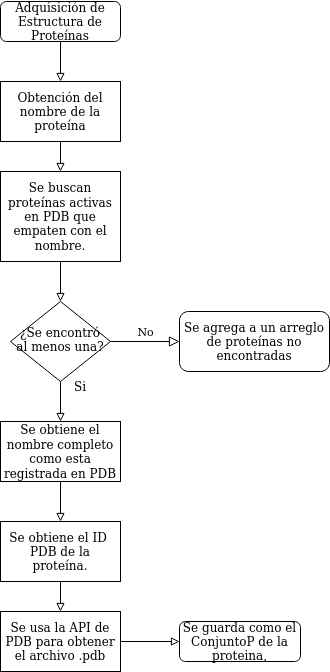
\includegraphics[scale=0.75]{Capitulo4/Documentos/imagenes_generacion/EstructuraPro.png}
    \caption{Diagrama de flujo de adquisición de la estructura de  Proteínas}
    \label{Adquisicion_estructura}
\end{figure}

\noindent Para el caso de la base de datos DrugBank, si bien es de libre acceso, su API no lo es, por lo que, para obtener información de los elementos contenidos en dicha base de datos se utiliza un método conocido como Web Scraping. 

\noindent Para realizar el método ya mencionado es usada la librería Selenium, este técnica es únicamente usada para adquirir la estructura pdb del compuesto, así como su actividad biológica.  Algo más que se debe aclarar es que para trabajar con Selenium es usado un driver para ser ocupado sobre un navegador web.\\

\noindent Para la adquisición de la estructura PDB, se ingresa a la página de drugbank, se realiza la búsqueda del compuesto, si éste existe, se procede a obtener un elemento html que  nos brinde la  dirección  web, a la cual se realiza un  request para conseguir su contenido, que es la estructura del compuesto. Esto queda mejor explicado en el siguiente diagrama.\\

\begin{figure}[H]
    \centering
    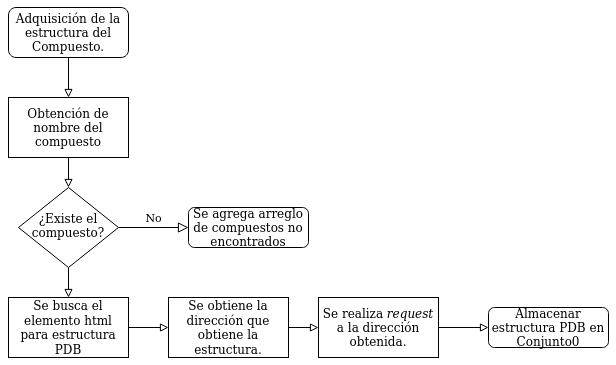
\includegraphics[scale=0.70]{Capitulo4/Documentos/imagenes_entorno/figura_flujo.png}
    \caption{Diagrama de flujo de adquisición PDB del compuesto haciendo uso de Web Scrapping.}
    \label{Diagrama_de_flujo_1}
\end{figure}

\noindent Junto con la estructura, la bio-actividad se adquiere por medio de  Drugbank y haciendo uso del Web Scrapping, una vez que se cuenta con el nombre del compuesto, se busca la sección de Actividad Biológica, para esto  de igual forma, ya se debe haber confirmado en el mismo proceso si el compuesto  existe. si en la página que muestra toda la información del compuesto, no se halla la sección deseada, se indica en  el archivo del conjunto 0 que no posee actividad, de existir la sección, se obtiene el contenido de la tabla, se realiza la conversión a una cadena de caracteres para ser guardada en el archivo  conjunto 0.

\begin{figure}[H]
    \centering
    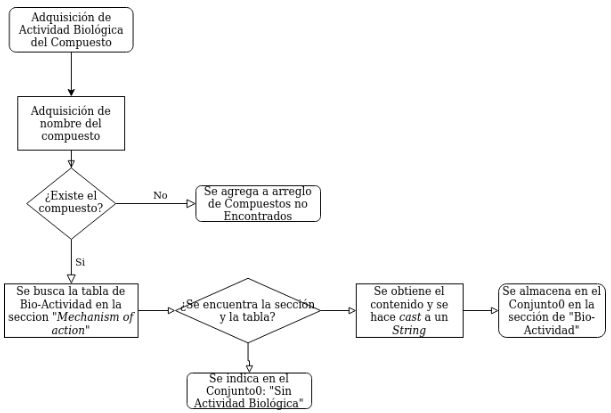
\includegraphics[scale=0.70]{Capitulo4/Documentos/imagenes_entorno/Actividad_biologica.png}
    \caption{Diagrama de flujo de adquisición de la Actividad Biológica}
    \label{Actividad_biologica}
\end{figure}

%%%%%%%%%%%%%%%%%%%%%%%%%%%%%%%%%%%%%%%%%%%%%%%%%%%%%%%%5
\subsubsection{Búsqueda concurrente}\label{concurrente}
\noindent El proceso de solicitar información a las API o realizar web scrapping, si bien no es complejo puede llegar a tomar algo de tiempo para recibir una respuesta del servidor que tienen las bases de datos. Para solucionar esta situación se utiliza la programación concurrente con hilos, los cuales evitan la latencia provocada por los tiempos que demoran las API en resolver las solicitudes que envía SisPAF. El programa crea un hilo por cada elemento que se obtuvo con la lectura del archivo inicial (tanto de compuestos como de proteínas). Cada hilo entonces tiene un elemento asociado del cual debe conseguir información mediante las peticiones a las API o el uso de web scrapping. Así, el tiempo requerido para realizar la búsqueda de información se reduce considerablemente.

\subsubsection{Construcción de conjuntos}
\noindent A la par de la actividad de búsqueda, una vez que la información es obtenida mediante las API’s, los hilos proceden a escribir esa información en archivos de texto. Para los compuestos, los hilos escriben la información en archivos de texto plano dentro de un directorio denominado Compounds, el cual está en el directorio donde se ha creado (o donde ya existe) el proyecto. Por su parte, la información de las proteínas es almacenada de la misma forma, solo que en un directorio de nombre Proteins. Los archivos que comprende el directorio Compounds forman el conjunto 0 (Véase \ref{diccionario}), mientras que todos los archivos que se encuentran en el directorio de Proteins forman el conjunto P (véase \ref{diccionario}).

\subsubsection{Manejo de pérdida de conexión a internet}
\noindent El manejo del error de conexión a internet está compuesto por tres partes. La primera parte es la detección de desconexión, que se realiza cuando alguna de las API’s o el proceso de webscrapping arrojan un error que se identifica como error de red. La segunda parte que toma lugar luego de que el error de red es identificado, es la de alerta al usuario de que no hay conexión a internet a la vez que se suspende el proceso de búsqueda, es decir, mientras no haya conexión las peticiones a las API’s y el webscrapping no son realizados pues los hilos se encuentran “dormidos”. La tercera parte es la reconexión la cual sucede cuando el usuario atiende la alerta emitida por el sistema, el cual como respuesta, realiza una rápida comprobación verificando si le es posible acceder al servidor central de Google. En caso de que le sea posible, el sistema emite una notificación para que todos los hilos que se encontraban pausados continúen con el proceso de la búsqueda de datos. Si por el contrario no es posible realizar la conexión al servidor de Google, la alerta vuelve a aparecer y el proceso de búsqueda se mantiene suspendido. La figura \ref{Desconexion} muestra el diagrama de flujo que sirvió como base para implementar la solución descrita en este apartado.

\begin{figure}[H]
    \centering
    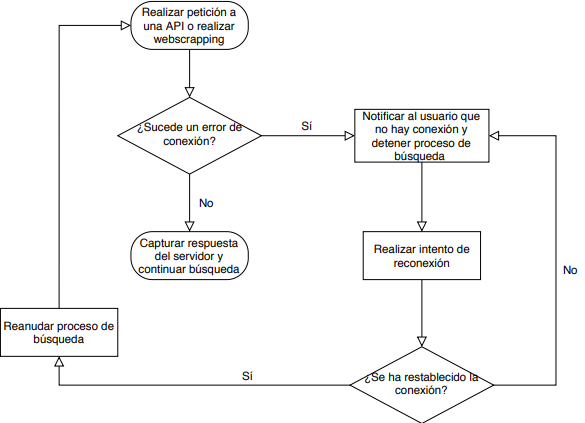
\includegraphics[scale=0.7]{Capitulo4/imagenes/diagramaDesconexion.png}
    \caption{Diagrama de flujo para el manejo de la pérdida de conexión a internet}
    \label{Desconexion}
\end{figure}

\subsubsection{Lectura de contenido de un proyecto}
\noindent Para el caso en el que el usuario desea abrir un proyecto ya existente, SisPAF solicita primero que se le indique el directorio donde se encuentra el proyecto. Acto seguido analiza la estructura de ese directorio para revisar que contenga los archivos que deben estar ahí puesto que si ya se ha creado un proyecto en ese directorio, deben existir ahí por lo menos el directorio de Compounds, el de Proteins y la copia del archivo inicial que genera el sistema (estos elementos se generan cuando se crea un nuevo proyecto). Si existen estos elementos procede a analizar el contenido de dichos directorios para determinar qué archivos faltan y que archivos se encuentran incompletos y requieren más información (esta lectura se realiza utilizando hilos para optimizar la tarea de leer varios archivos, se sigue la idea descrita en el apartado \ref{concurrente}). Una vez hecho esto se procede a continuar con el proceso ya sea de búsqueda o análisis dependiendo de la robustez actual del proyecto en cuestión. Si el sistema detecta un archivo final (Tabla \ref{diccionario}) no procede a abrir dicho proyecto pues este archivo es la muestra de que el proyecto ya ha sido terminado. La figura \ref{abrir} describe el diagrama de flujo que sigue el proceso de abrir un proyecto existente.

\begin{figure}[H]
    \centering
    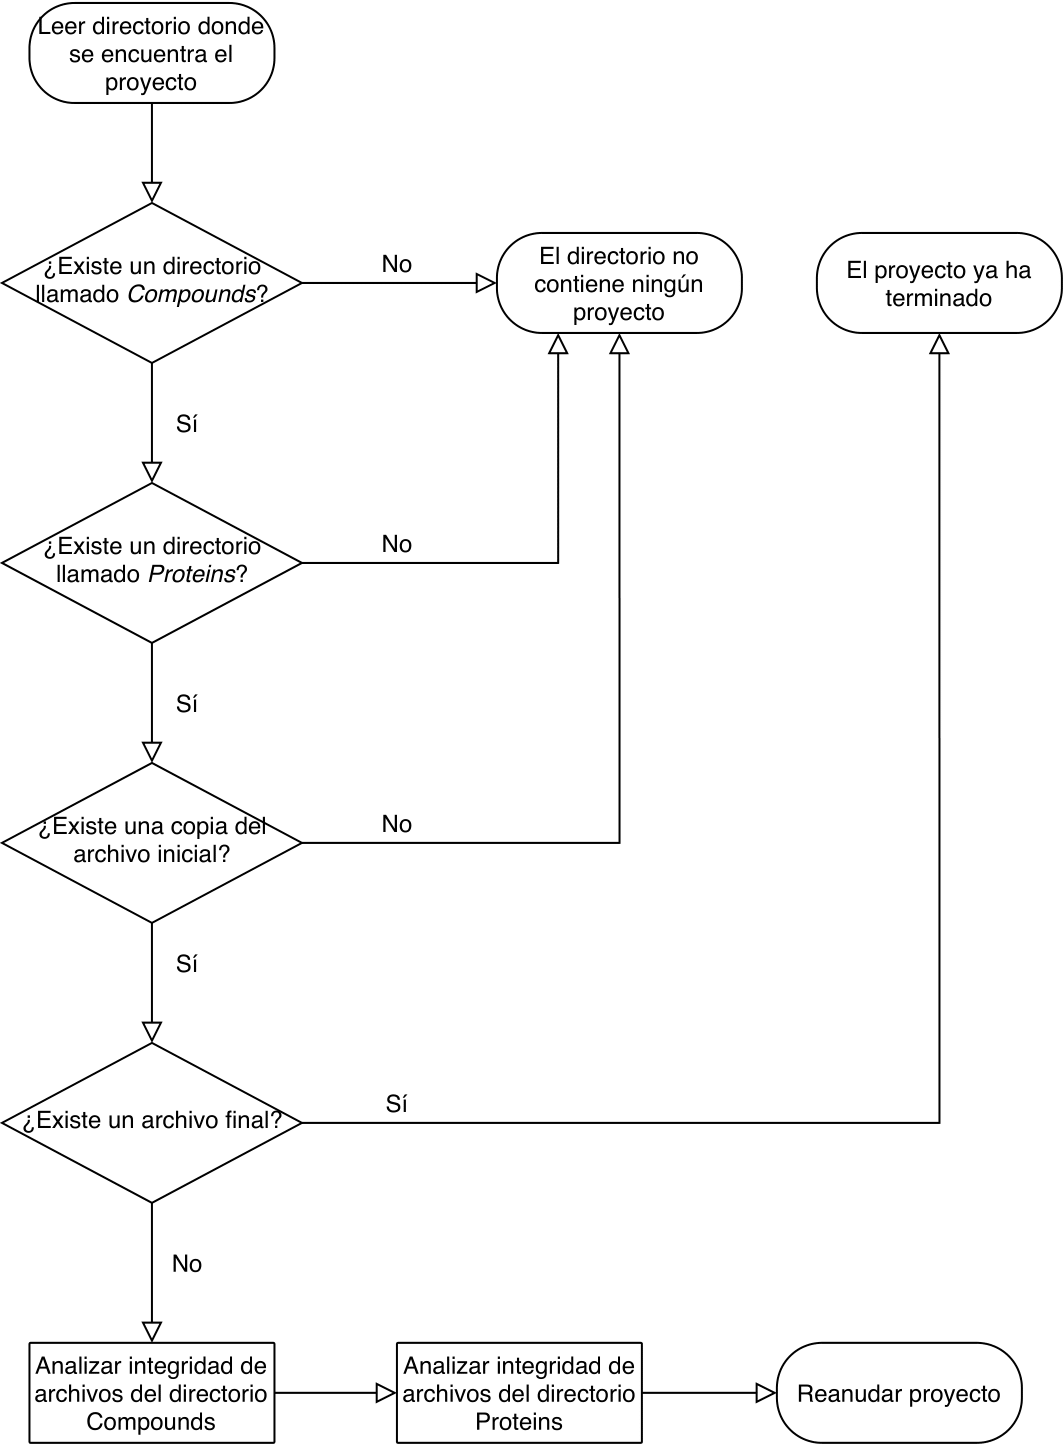
\includegraphics[scale=0.3]{Capitulo4/imagenes/diagramaAbrirProy-1.png}
    \caption{Diagrama de flujo que sigue SisPAF cuando se solicita abrir un proyecto ya existente.}
    \label{abrir}
\end{figure}
%%%%%%%%%%%%%%%%%%%%%%%%%%%%%%%%%%%%%%%%%%%%%%%%%%%%%
\subsection{Análisis de información}
\subsubsection{Diseño de interfaces}{
\noindent En la sección de análisis, donde el sistema hace uso de toda la información recolectada, se planificó una interfaz muy similar a la que se muestra durante el proceso de la búsqueda de información, una pantalla de espera,  para hacerle saber al usuario que el sistema  continúa trabajando, la comparación se muestra a continuación.

\begin{figure}[H]
    \centering
    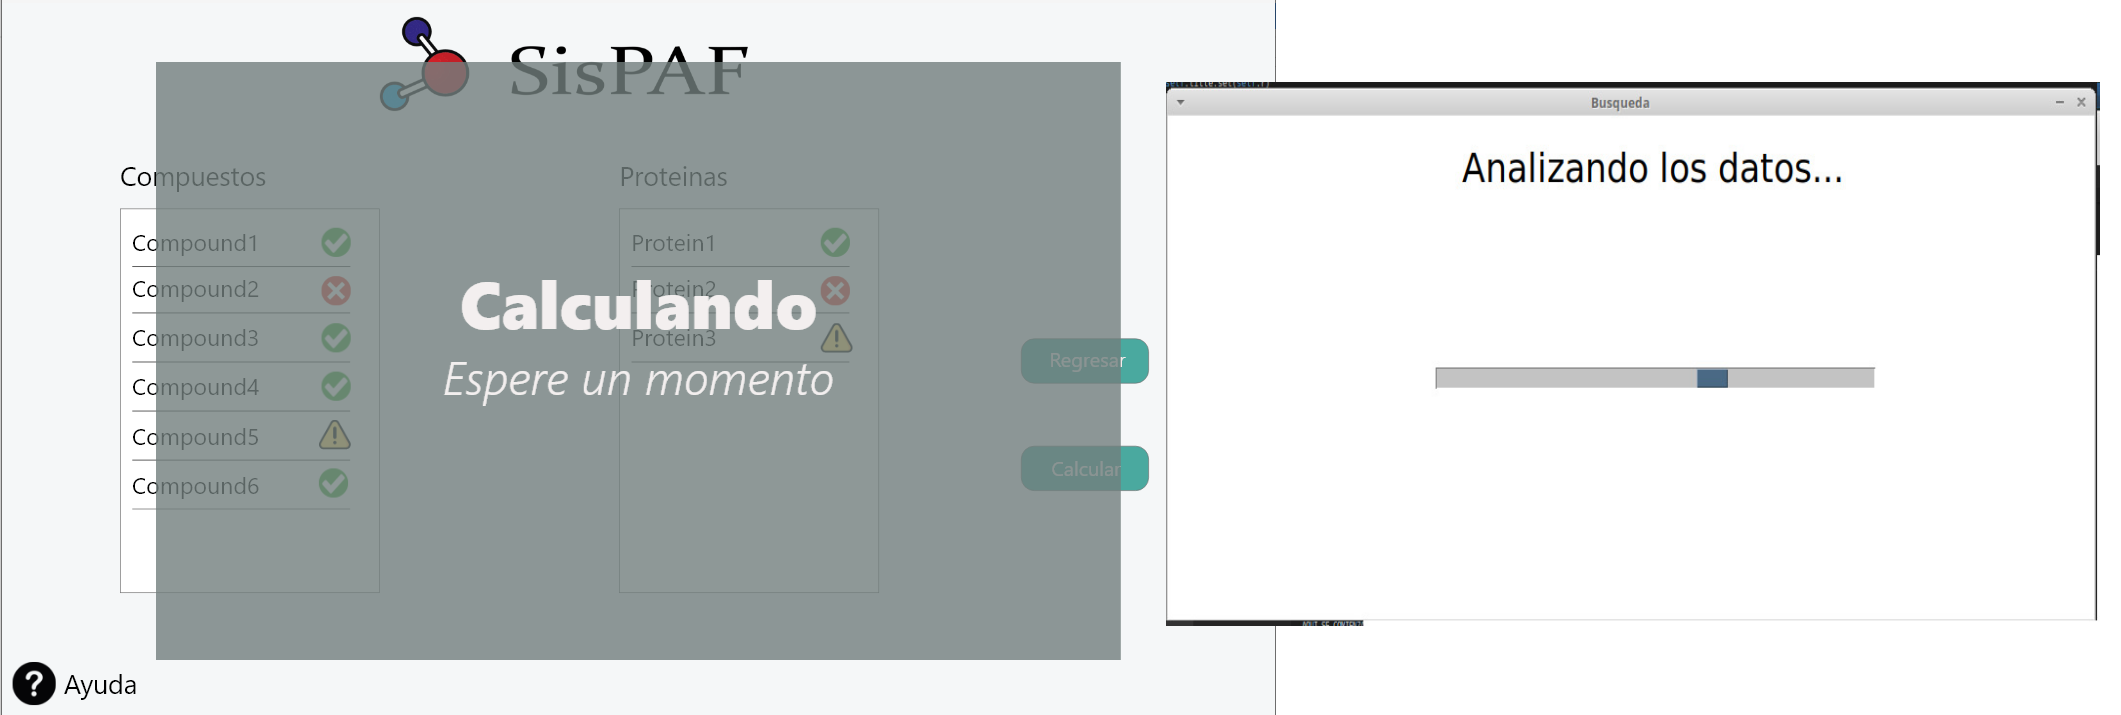
\includegraphics[scale=0.27]{Capitulo4/Documentos/imagenes_generacion/Analisis.png}
    \caption{Comparación de pantallas para el análisis de datos, a la izquierda la planeada y a la derecha la programada.}
    \label{comparacion_6l}
\end{figure}
}
\subsubsection{Análisis multiproceso}{
\noindent El desarrollo del proceso del análisis de la información es considerado exhaustivo de CPU, es decir, este proceso requiere una considerable capacidad de procesamiento del equipo de cómputo. Contrario a la aplicación concurrente con hilos, para los procesos que involucran en uso considerable de recursos de procesamiento se emplea el método de multiprocesos. El uso de múltiples procesos para el módulo de análisis de información supone una reducción considerable en los tiempos de procesamiento. Aquí se toman en cuenta dos cosas, la primera es la cantidad de procesos y la división de tareas, ya que el número de procesos que se debe crear corresponde con el número de núcleos físicos del equipo de cómputo, y a su vez las tareas a realizar deben asignarse a cada uno de los procesos creados. La segunda cosa a tomar en cuenta es la ventaja de un trabajo en paralelo. El uso de múltiples procesos permite una paralelización de las actividades que debe realizar el sistema, es decir, si se tienen 4 núcleos, se pueden realizar al mismo tiempo (de manera paralela) 4 actividades, aprovechando al 100\% la capacidad de procesamiento del equipo de cómputo donde se está ejecutando el sistema.



}
\subsubsection{\textit{Docking}}{
\noindent En el campo de modelado molecular (acoplamiento molecular) es un método que predice la conformación preferida de una molécula, al estar unida a otra, con el fin de formar un complejo estable.\cite{15}\\
\noindent La simulación de este procedimiento es un proceso complicado. En este enfoque, la proteína y el ligando están separados por una distancia física, y el ligando encuentra su posición en el sitio activo de la proteína luego de un cierto número de ''movimientos'' en su espacio conformacional. Los movimientos incorporan al cuerpo rígido transformaciones tales como el traslado y rotaciones. Cada uno de estos movimientos, en el espacio conformacional del ligando, induce un costo energético al sistema, y por tanto después de cada movimiento, se calcula la energía total del sistema.\\

\noindent Para hacer un examen de acoplamiento, primero se necesita la estructura de la proteína. Normalmente la estructura ha sido determinada usando una técnica biofísica como la cristalografía de rayos X, o menos frecuente, una Espectroscopia de resonancia magnética nuclear. La estructura de esta proteína y la de los ligandos potenciales sirven como los valores a ingresar en el programa que calcula el acoplamiento. El éxito del programa depende de dos factores: el algoritmo de búsqueda y la función de puntuación.\\

\noindent Para el acoplamiento molecular usamos una herramienta llamada AutoDock Vina la cual permite calcular de manera automática cada uno de estos movimientos. Para generar el resultado de \textit{Docking} con vina, pide como parámetros un archivo donde se configuran las entradas al sistemas y que esperas como salida del mismo, un ejemplo de este archivo, está ilustrado en la figura \ref{dock_ing}.\\

\noindent Como salida tendremos un archivo PDBQT el cual nos da el valor del acoplamiento molecular en distintas iteraciones, a estos valores los llamaremos “Deltas” los cuales son una pieza fundamental para implementar el algoritmo de regresión lineal, ya que estos datos se convertirán en nuestra variable dependiente.

\begin{figure}[H]
    \centering
    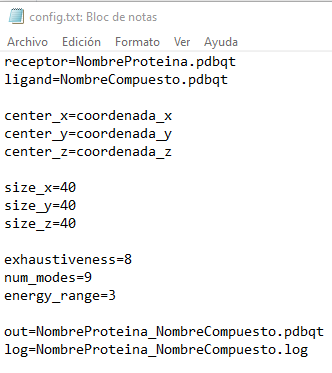
\includegraphics[scale=.99]{Capitulo4/Documentos/imagenes_entorno/archivo_entrada.png}
    \caption{Archivo de configuración para\textit{Docking}.}
    \label{dock_ing}
\end{figure}

\noindent Como podemos ver, Vina pide como parámetros de entrada la estructura 3D de un receptor (molécula que recibe, por lo normal es una proteína u otro biopolímero) y la estructura 3D del ligando (molécula que se enlaza al receptor. Por lo general son moléculas más pequeñas que el receptor, aunque también pueden ser otro biopolímero).\\

\noindent De igual manera Vina pide como parámetros el centro del receptor, estas coordenadas las podemos generar a través de una herramienta de MGLTools (mismo desarrollador de AutoDockTools) la cual se encuentra dentro del archivo “prepare\_gpf4.py”, esta biblioteca nos permite generar las coordenadas ideales del centro del receptor, las cuales son indispensables para generar el \textit{Docking}, para utilizar esta biblioteca debemos tener las estructuras 3D del receptor y ligando en formato PDBQT por lo cual debemos realizar una conversión de estas estructuras ya que SysPAF las obtiene pero en su formato PDB.\\

\noindent Para realizar esta conversión, es necesario usar la biblioteca de MGLTools la cual transforma la estructura de la proteína y la prepara para ser receptora, al igual que cambia el formato de PDB a PDBQT. Esta biblioteca la podemos encontrar dentro del archivo “prepare\_receptor.py” para el caso de la transformación de un receptor ya que si se desea convertir la estructura de un ligando (estructura de un compuesto en el caso de SysPAF) es necesario utilizar el archivo “prepare\_ligand.py”.\\

\noindent La figura \ref{flujo_dock} muestra el flujo que sigue SysPAF para realizar el proceso de \textit{Docking}.

\begin{figure}[H]
    \centering
    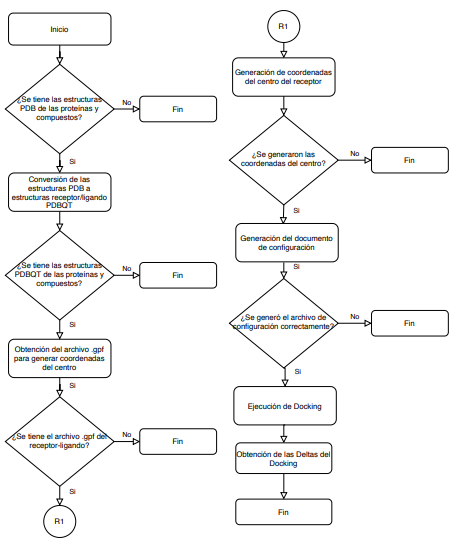
\includegraphics[scale=.65]{Capitulo4/Documentos/imagenes_entorno/docking-flujo.png}
    \caption{Flujo que sigue SysPAF para realizar el proceso de \textit{Docking}.}
    \label{flujo_dock}
\end{figure}

}

\subsubsection{Implementación de algoritmos de \textit{Machine Learning}}{
\noindent El uso de algoritmos de Machine Learning permite la generación de modelos para realizar cálculos más rápidos en términos de predicción de la efectividad de los compuestos de estudio.El uso de algoritmos de \textit{Machine Learning} permite la generación de modelos para realizar cálculos más rápidos. Los modelos se obtienen a partir de una regresión lineal múltiple que toma como variables independientes a los valores de las propiedades físicas y químicas de cada medicamento. La variable dependiente está definida por el valor de delta G obtenido del proceso del \textit{Docking}. Luego de obtener los coeficientes de la regresión lineal, estos son almacenados en un archivo el cual contiene todos los modelos para las distintas clasificaciones de medicamentos (cada clasificación constituye un modelo). Una vez definido el modelo, el proceso del \textit{Docking} y de la regresión lineal puede omitirse en caso de volver a tener que realizar un análisis de información en el cual, luego de revisar el archivo donde se almacenan los modelos, se encuentre el modelo para la clase de compuestos que se están analizando. La figura \ref{Machine} muestra una ilustración del proceso previamente descrito.

\begin{figure}[H]
    \centering
    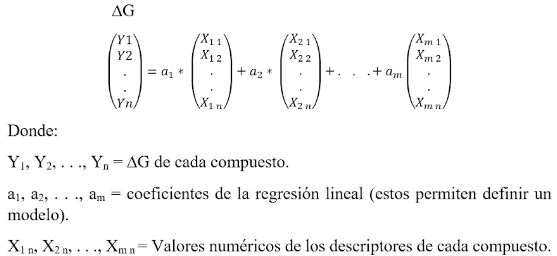
\includegraphics[scale=0.70]{Capitulo4/Documentos/imagenes_entorno/regresion_lineal.png}
    \caption{Forma de implementar la regresión lineal y su relación con los resultados del \textit{Docking}.}
    \label{Machine}
\end{figure}
\noindent Una vez que la regresión lineal es finalizada, el sistema guarda dicho modelo en una carpeta el cual puede recuperar en caso de que se solicite analizar datos correspondientes a una clasificación que corresponda con algún modelo de regresión lineal existente. Al recuperar el modelo correspondiente, se puede simplemente realizar el proceso de predicción directa de la variable Y, dado que en ese modelo se observan ya los coeficientes y las variables independientes X que están determinadas por los descriptores del nuevo conjunto 0 a analizar.
}
\subsubsection{Precisión del modelo de regresión lineal generado}{
\noindent La evaluación de qué tan acertado es el modelo de regresión lineal que se genera luego de aplicar el algoritmo del mismo nombre se basa en la obtener y medir la influencia de los errores en la exactitud del modelo de regresión lineal. Estos errores, si bien se implementan de manera directa gracias a las herramientas de la biblioteca de python sklearn, requieren de su correcta comprensión para poder entender qué tan exacto es el modelo y por qué.\\
\noindent La estadística ha desarrollado medidas resumidas que toman la colección de residuos del modelo (valor actual - valor esperado) y los condensan en un solo valor que representa la capacidad predictiva del modelo implementado. De estas medidas se han considerado 3: Error Medio Absoluto (MAE, por sus siglas en inglés, Mean Absolute Error), Error Cuadrático Medio (MSE, por sus siglas en inglés, Mean Square Error) y Raíz del Error Cuadrático Medio (RMSE, por sus siglas en inglés, Root Mean Square Error).\cite{16}\\

\noindent El error medio absoluto se obtiene mediante la sumatoria de cada valor absoluto del residual (diferencia entre el valor predicho y el valor esperado), y luego dividiendo entre el número de muestras. Este error  se refiere a la media de los valores absolutos de cada error de predicción en todas las instancias del conjunto de datos de prueba.\\
\noindent Para el caso de error medio cuadrado permite determinar qué tan cerca está una línea de regresión de un conjunto de puntos. Lo hace tomando las distancias desde los puntos hasta la línea de regresión (estas distancias son los "errores") y cuadrándolos. La cuadratura es necesaria para eliminar cualquier signo negativo. También le da más peso a las diferencias más grandes (outliers).\\

\noindent Por último, considerando que el error cuadrático medio es la desviación estándar de los residuos y sabiendo que los residuos son una medida de qué tan lejos están los puntos de datos de la línea de regresión, la raíz del error cuadrático medio es una medida de la dispersión de estos residuos. En otras palabras, dice qué tan concentrados están los datos alrededor de la línea de regresión.\\

\begin{figure}[H]
    \centering
    \includegraphics[scale=0.85]{}
    \caption{Representación matemática del error medio absoluto.}
    \label{ecuaciones}
\end{figure}

\begin{figure}[H]
    \centering
    \includegraphics[scale=0.85]{}
    \caption{Representación matemática del error cuadrático medio.}
    \label{ecuaciones}
\end{figure}

\begin{figure}[H]
    \centering
    \includegraphics[scale=0.85]{}
    \caption{Representación matemática de la raíz del error cuadrático medio.}
    \label{ecuaciones}
\end{figure}

\noindent Los errores previamente definidos se utilizan con la observación de que a menor valor, mejor. Es decir, que estos 3 valores resulten en 0 indicaría que el modelo es perfecto. Las pruebas para obtener estos errores se realizaron con los conjuntos de datos indicados que en anexo X. Y en promedio, de X pruebas se obtuvieron los resultados que ilustra la tabla siguiente.



\begin{longtable}{|c|c|c|c|c|c|}
\caption{Resultados de las mediciones de errores realizadas..}\\ 
\hline
\multirow{}{}{\textbf{Clasificación} } & \multicolumn{2}{c|}{\textbf{Número de muestras} } & \multirow{}{}{\textbf{MAE} } & \multirow{}{}{\textbf{MSE} } & \multirow{}{}{\textbf{RMSE} }  \\* 
\cline{2-3}
                                         & \textbf{Entrenamiento} & \textbf{Prueba}          &                                &                                &                                  \endfirsthead 
\hline
Anti-inflamatorio                        & 12                     & 4                        & 0.471                          & 0.472                          & 0.687                            \\ 
\hline
Antiviral                                & 4                      & 2                        & 2.583                          & 6.673                          & 2.583                            \\ 
\hline
Antiandrogénico                          & 2                      & 1                        & 0.82                           & 0.67                           & 0.82                             \\ 
\hline
Cardiovascular                           & 6                      & 2                        & 6.903                          & 72.383                         & 8.507                            \\ 
\hline
Antifúngico                              & 5                      & 2                        & 6.230                          & 39.48                          & 6.272                            \\ 
\hline
Antihipertensivo                         & 18                     & 5                        & 4.934                          & 39.784                         & 6.307                            \\ 
\hline
Antiparasitario                          & 7                      & 2                        & 0.46                           & 0.313                          & 0.56                             \\ 
\hline
Antibiótico                              & 4                      & 2                        & 2.353                          & 10.124                         & 3.181                            \\ 
\hline
Antiepiléptico                           & 5                      & 2                        & 0.03                           & 0.001                          & 0.032                            \\ 
\hline
Anticoagulante                           & 5                      & 2                        & 0.334                          & 0.133                          & 0.364                            \\ 
\hline
\textbf{Total}                           & \textbf{68}            & \textbf{24}              & \textbf{2.511}                 & \textbf{17.003}                & \textbf{2.931}                   \\
\hline
\end{longtable}

\noindent De estos resultados se puede decir que el modelo generado tiene un margen de error de 2.5 unidades, esto es, la variación entre el valor que se espera obtener y el valor que puede predecir el modelo está definida en un rango de 0 a 2.5, y considerando la cantidad de pruebas, se puede concluir que el modelo es eficaz.\\

\noindent Algo muy importante que se debe mencionar es que el modelo de regresión lineal depende en gran medida de la calidad y la cantidad de datos proporcionados. Un modelo con muchas variables independientes para trabajar pero que son pobres en cuanto a la relación cualitativa de estas variables con las variables dependientes resultan en un modelo predictivo poco preciso, por otro lado un modelo donde las variables dependientes tengan mucha influencia en la variable dependiente además de grandes muestras de información para entrenar y probar el modelo derivan en la generación de un modelo más preciso y robusto.
}

%%%%%%%%%%%%%%%%%%%%%%%%%%%%%%%%%%%%%%%%%%%%%%%%%%%%%
\subsection{Generación de resultados}
\subsubsection{Diseño de interfaces}
\noindent La interfaz de despliegue de resultados fue desarrollada con la finalidad de que el usuario pueda visualizar los resultados obtenidos por el sistema, los resultados están desplegados en una tabla de dos columnas, la columna uno lleva por nombre “Compuesto”, donde se en-lista el nombre de cada compuesto, la columna dos tiene el nombre de “Efectividad”, esta muestra los efectos que tuvo el compuesto para “destruir” la proteína, está  representada numéricamente. 

\begin{figure}[H]
    \centering
    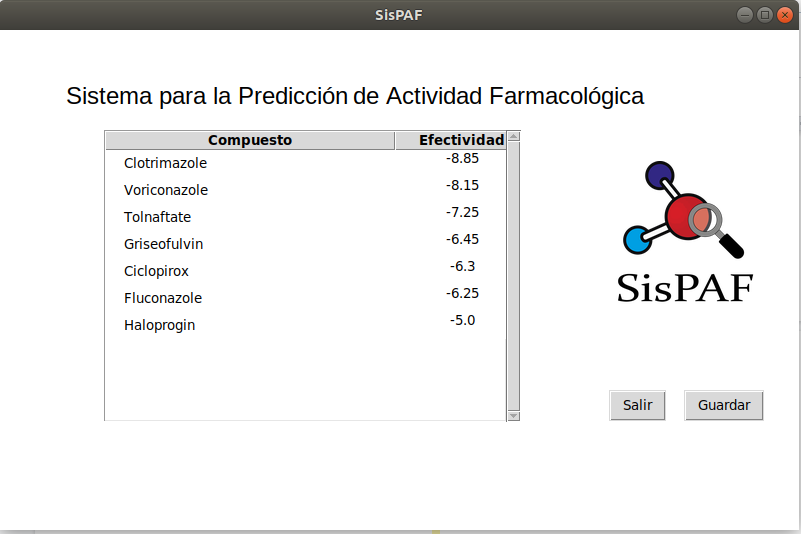
\includegraphics[scale=0.52]{Capitulo4/Documentos/imagenes_generacion/imagen-2-2-7-2.png}
    \caption{Despliegue de resultados.}
    \label{Des_Res}
\end{figure}

\noindent La columna “Efectividad” nos ayudará a ordenar los resultados, ya que se tomará el valor más alto y este será nuestro punto de partida para desplegar nuestros resultados de forma descendente.

\subsubsection{Ordenamiento de resultados:}
\noindent Para el ordenamiento de los resultados, utilizamos una estructura de datos llamada “diccionario” en python, dicha estructura soporta cualquier tipo de dato como enteros, cadenas, listas e incluso otras funciones. La ventaja de utilizar este tipo de estructura es el poder identificar cada elemento por una clave (key) ya que está dada por duplas.

\noindent Donde tomamos el nombre del compuesto como la llave de la dupla y la efectividad como el valor. Para acceder a cada uno de los valores del diccionario de datos, es necesario poner el nombre de la clave (compuesto), lo cual nos permite eliminar la redundancia de datos, ya que esta estructura no guarda datos duplicados.

\subsubsection{Construcción de archivo de resultados:}
\noindent La Para evitar una pérdida de datos, se definió una función que nos permite guardar los resultados obtenidos por el sistema en un archivo txt, dicho archivo se encuentra guardado en una carpeta que lleva por nombre “Resultados” y a su vez este lleva por nombre “Resultados\_Proyecto.txt”. El archivo contiene una estructura similar a la tabla que se muestra en la interfaz de despliegue de resultados y de igual manera está ordenada de mayor a menor efectividad.

\begin{figure}[H]
    \centering
    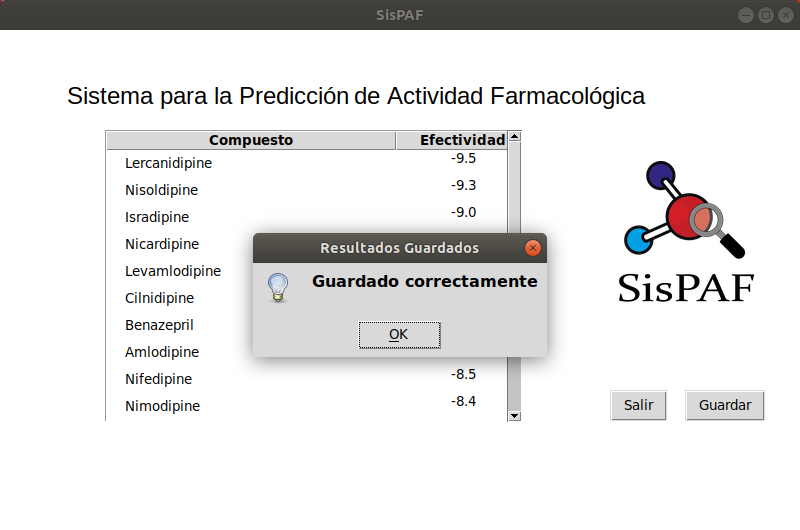
\includegraphics[scale=0.52]{Capitulo4/Documentos/imagenes_generacion/imagen-2-2-8-1.png}
    \caption{Ejemplo de archivo guardado.}
    \label{fig:my_label}
\end{figure}

\subsubsection{Alertas y errores:}
\noindent La interfaz de “despliegue de resultados” cuenta con dos tipos de alertas, las cuales se muestran al efectuar una interacción específica con el sistema, describiremos a continuación dichas alertas de manera individual:

\noindent\textit{Resultados guardados:}\\

\noindent El sistema SisPAF muestra una alerta, cuando el documento fue guardado correctamente, esta acción surge de dar clic en el botón “Guardar” de la interfaz. El objetivo principal de desarrollar esta funcionalidad es notificar al usuario que la acción que realizó fue efectuada con éxito.\\

\begin{figure}[H]
    \centering
    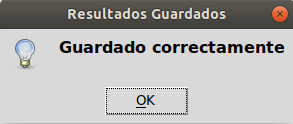
\includegraphics[scale=0.85]{Capitulo4/Documentos/imagenes_generacion/manual_3.png}
    \caption{Resultados guardados correctamente}
    \label{resultados_guard}
\end{figure}

\noindent \textit{Resultados no guardados:}\\

\noindent El sistema SisPAF muestra una alerta que nos permite decidir si seguir con la acción que el usuario seleccionó, dicha acción puede estar descrita por un cierre forzado del sistema, dar clic en el botón “Inicio” o seleccionar el botón de “Salir” que fue implementado en el sistema, todo esto antes de guardar el documento de resultados. El objetivo de esta notificación es poder alertar al usuario de que sus resultados no han sido guardados y de seguir con esta acción podrían perderse y tendrían que ser calculados nuevamente.

\begin{figure}[H]
    \centering
    
\includegraphics[scale=0.85]{Capitulo4/Documentos/imagenes_generacion/manual_4.png}
    \caption{Alerta de acción.}
    \label{resultados_guard}
\end{figure}

%%%%%%%%%%%%%%%%%%%%%%%%%%%%%%%%%%%%%%%%%
\section{Ejecución de las Pruebas Unitarias}

%%%%%%%%%%%%%%%%%%%%%%%%%%%%%%%%%%%%%%%%%%%%
%% Please add the following required packages to your document preamble:
% \usepackage{longtable}
% Note: It may be necessary to compile the document several times to get a multi-page table to line up properly
\begin{longtable}{|l|l|}
\caption{Prueba unitaria RF1.1}
\label{PU_RF1_1}\\
\hline

\textbf{Requerimiento Funcional}                                                       & \textbf{RF1.1 Adquisición del archivo base.}                                                                                                                                                                                                                                                                                                                                                                                                                                                                                                                                                                                                                                                     \\ \hline
\endfirsthead
%
\multicolumn{2}{c}%
{{\bfseries Tabla \thetable\ Continuación de la página anterior}} \\
\endhead
%
\textbf{Perfiles Implicados}                                                           & \begin{tabular}[c]{@{}l@{}}- Desarrollador.\\ - Tester.\end{tabular}                                                                                                                                                                                                                                                                                                                                                                                                                                                                                                                                                                                                                             \\ \hline
\textbf{Planificación temporal}                                                        & \begin{tabular}[c]{@{}l@{}}1. Prueba de compilación.\\ 2. Prueba de funcionamiento.\\ 2.1 Func. botón adquisición archivo.\\ 2.2 Muestra de pantalla selección de\\ archivo.\\ 2.3 Acceso a directorio.\\ 2.4 Carga de archivo.\\ 2.5 Func. botón buscar.\end{tabular}                                                                                                                                                                                                                                                                                                                                                                                                                           \\ \hline
\textbf{Criterio de verificación}                                                      & \begin{tabular}[c]{@{}l@{}}1. Compilación del código.\\ 2. Ejecutable del módulo, hay muestras\\ de que el código hace algo (algo: definido por los \\ siguientes puntos).\\ 2.1 Funcionamiento del botón de Archivo base.\\ 2.2 Visualización de selección de archivo.\\ 2.3 Acceso al directorio correcto o permite acceder \\ a uno distinto desde la pantalla de selección de \\ archivo.\\ 2.4 Carga del archivo correcto.\\ 2.5 El botón se ve adecuadamente y accede al\\ archivo indicado y logra una lectura correcta.\end{tabular}                                                                                                                                                     \\ \hline
\textbf{Criterio de aceptación}                                                        & \begin{tabular}[c]{@{}l@{}}1. No hay errores que impidan la compilación \\ del código.\\ 2. Al usar el ejecutable del módulo, hay muestras \\ de que el código hace algo \\ (algo: definido por los siguientes puntos).\\ 2.1 Se muestra el botón correspondiente, y realiza la \\ acción indicada.\\ 2.2 Es visualizada la pantalla de selección de archivos \\ con cada uno de los componentes.\\ 2.3 La selección de archivos se encuentra en el \\ directorio correcto o permite acceder a uno distinto.\\ 2.4 Solo permite la carga de un archivo de texto \\ plano, y es cargado adecuadamente.\\ 2.5 El botón se ve adecuada, y realiza la acción \\ indicada correctamente.\end{tabular} \\ \hline
\textbf{\begin{tabular}[c]{@{}l@{}}Definición de\\ verificaciones\end{tabular}}        & \begin{tabular}[c]{@{}l@{}}- Errores de Compilación: Ocurren porque la sintaxis \\ del lenguaje no es correcta, de cajón este tipo de \\ errores no permiten que la aplicación se ejecute. \\ \\ - Acción de botón: representa un botón que, cuando \\ es presionado, envía información al que pertenece. \\ La función de  un botón representada  el contenido\\ del elemento.\\ \\ -Visualización de pantalla interfaz de usuario.\end{tabular}                                                                                                                                                                                                                                                \\ \hline
\textbf{\begin{tabular}[c]{@{}l@{}}Análisis y evaluación\\ de resultados\end{tabular}} &                                                                                                                                                                                                                                                                                                                                                                                                                                                                                                                                                                                                                                                                                                  \\ \hline
\textbf{Productos  a entregar}                                                         & \begin{tabular}[c]{@{}l@{}}- Adquisición del archivo base funcionando \\ correctamente.\end{tabular}                                                                                                                                                                                                                                                                                                                                                                                                                                                                                                                                                                                             \\ \hline

\end{longtable}
% Please add the following required packages to your document preamble:
% \usepackage{longtable}
% Note: It may be necessary to compile the document several times to get a multi-page table to line up properly
\begin{longtable}{|l|l|}
\caption{Caso de prueba RF1}
\label{CP_RF1}\\
\hline
\textbf{ID del Caso de prueba}                                                          & CPRF1                                                                                                                                                            \\ \hline
\endfirsthead
%
\multicolumn{2}{c}%
{{\bfseries Tabla \thetable\ Continuación de la página anterior}} \\
\endhead
%
\textbf{Versión}                                                                        & 1.0                                                                                                                                                              \\ \hline
\textbf{Nombre}                                                                         & Caso de prueba para adquisición de archivo base.                                                                                                                 \\ \hline
\textbf{\begin{tabular}[c]{@{}l@{}}Identificador de \\ requerimiento\end{tabular}}      & RF1.1                                                                                                                                                            \\ \hline
\textbf{Propósito}                                                                      & \begin{tabular}[c]{@{}l@{}}Determinar capacidad del sistema para \\ obtener el archivo base.\end{tabular}                                                        \\ \hline
\textbf{Dependencias}                                                                   & N/A                                                                                                                                                              \\ \hline
\textbf{\begin{tabular}[c]{@{}l@{}}Ambiente de \\ prueba/configuración\end{tabular}}    & \begin{tabular}[c]{@{}l@{}}- Hardware: Equipo de computo\\ (preferentemente portatíl)\\ - Software: Compilador python3, \\ IDE y/o editor de texto.\end{tabular} \\ \hline
\textbf{Inicialización}                                                                 & \begin{tabular}[c]{@{}l@{}}- Codificación correspondiente al \\ requerimiento.\\ - Creación del archivo base.\end{tabular}                                       \\ \hline
\textbf{Finalización}                                                                   & N/A                                                                                                                                                              \\ \hline
\textbf{Acciones}                                                                       & \begin{tabular}[c]{@{}l@{}}. Compilar el código correspondiente.\\ - Colocar el archivo en el directorio \\ especificado.\end{tabular}                           \\ \hline
\textbf{\begin{tabular}[c]{@{}l@{}}Descripción de los \\ datos de entrada\end{tabular}} & \begin{tabular}[c]{@{}l@{}}- Archivo de texto plano.\\ - Directorio de la ubicación del archivo base.\end{tabular}                                               \\ \hline
\textbf{Salida esperada}                                                                & \begin{tabular}[c]{@{}l@{}}- Notificación de adecuada adquisición del \\ archivo base.\end{tabular}                                                              \\ \hline
\textbf{Salida obtenida}                                                                &  \begin{tabular}[c]{@{}l@{}}- Cuadro de diálogo para la obtención de archivos.\\
- Diálogo para indicar que un archivo es incorrecto.\\
- Sin diálogo para cuando el archivo es correcto;\\ Se sustituye por la habilitación de botón de inicio.\end{tabular}                                                                                                                                              
\\ \hline
\textbf{Resultado}                                                                      & \begin{tabular}[c]{@{}l@{}}- El módulo funciona adecuadamente,
aparecen los \\diálogos necesarios para la
interpretación  del usuario.\end{tabular}                                                                                                                                               
\\ \hline
\textbf{Severidad}                                                                      & - Baja                                                                                                                                                      \\ \hline
\textbf{Evidencia}                                                                      &   \begin{tabular}[c]{@{}l@{}} Evidencia en la imagen \ref{CPRF1}.\end{tabular}                                                                                                                                                            \\ \hline
\textbf{Estado}                                                                         & Iniciado                                                                                                                                                    \\ \hline
\end{longtable}
%%%%%%%%%%%%%%%%%%%%%%%%%%%%%%%%%%%%%%%%%%%%
%% Please add the following required packages to your document preamble:
% \usepackage{longtable}
% Note: It may be necessary to compile the document several times to get a multi-page table to line up properly
\begin{longtable}{|l|l|}
\caption{Prueba unitaria RF1.2}
\label{PU_RF1_2}\\
\hline
\textbf{Requerimiento Funcional}                                                       & \textbf{RF1.2 Búsqueda de los compuestos indicados..}                                                                                                                                                                                                                                                                                                                                                                                                                                                                                                                                  \\ \hline
\endfirsthead
%
\multicolumn{2}{c}%
{{\bfseries Table \thetable\ Continuación de la página anterior}} \\
\endhead
%
\textbf{Perfiles Implicados}                                                           & \begin{tabular}[c]{@{}l@{}}- Desarrollador.\\ - Tester.\end{tabular}                                                                                                                                                                                                                                                                                                                                                                                                                                                                                                                   \\ \hline
\textbf{Planificación temporal}                                                        & \begin{tabular}[c]{@{}l@{}}1. Prueba de compilación.\\ 2. Prueba de funcionamiento.\\ 2.1 Verificar adecuada lectura del archivo base\\ (token “compunds” ).\\ 2.2 Comprobar conexión a la base de datos \\ “DrugBank”.\\ 2.3 Obtención del .pdb de cada uno de los \\ compuestos enlistados.\\ 2.4 Almacenado del .pdb en el sistema.\end{tabular}                                                                                                                                                                                                                                   \\ \hline
\textbf{Criterio de verificación}                                                      & \begin{tabular}[c]{@{}l@{}}1. Compilación del código.\\ 2. Ejecutable del módulo, hay muestras de que el \\ código hace algo\\ (algo: definido por los siguientes puntos).\\ 2.1 Lectura del token que describe los nombres del\\ compuesto en el archivo base.\\ 2.2 Conexión a  DrugBank y por lo tanto a Internet.\\ 2.3 Adquirir el archivo .pdb del compuesto correcto.\\ 2.4 Almacenamiento de un archivo íntegro en el \\ sistema.\end{tabular}                                                                                                                                \\ \hline
\textbf{Criterio de aceptación}                                                        & \begin{tabular}[c]{@{}l@{}}1. No hay errores que impidan la compilación del \\ código.\\ 2. Al usar el ejecutable del módulo, hay muestras \\ de que el código hace algo\\ (algo: definido por los siguientes puntos).\\ 2.1 No se pierde ningún valor ni dato existente en el\\ archivo base.\\ 2.2 El sistema informa la correcta conexión a \\ “DrugBank”.\\ 2.3 El sistema informa que el compuesto existe \\ en la base de datos y confirma la adquisición \\ del .pdb.\\ 2.4 El sistema notifica la correcta obtención del \\ archivo .pdb y correcto  almacenado.\end{tabular} \\ \hline
\textbf{\begin{tabular}[c]{@{}l@{}}Definición de\\ verificaciones\end{tabular}}        & \begin{tabular}[c]{@{}l@{}}- Errores de Compilación: Ocurren porque la sintaxis \\ del lenguaje no es correcta, de cajón este tipo de \\ errores no permiten que la aplicación se ejecute. \\ \\ - Conexión a base de datos online:Una conexión a \\ base de datos es un archivo de configuración donde \\ se especifica los detalles físicos de una base de datos \\ como por ejemplo el tipo de base de datos y la \\ versión, y los parámetros que permiten una conexión\end{tabular}                                                                                               \\ \hline
\textbf{\begin{tabular}[c]{@{}l@{}}Análisis y evaluación\\ de resultados\end{tabular}} &                                                                                                                                                                                                                                                                                                                                                                                                                                                                                                                                                                                        \\ \hline
\textbf{Productos  a entregar}                                                         & \begin{tabular}[c]{@{}l@{}}- Búsqueda de los compuestos indicados \\ funcionando correctamente.\end{tabular}                                                                                                                                                                                                                                                                                                                                                                                                                                                                           \\ \hline
\end{longtable}
% Please add the following required packages to your document preamble:
% \usepackage{longtable}
% Note: It may be necessary to compile the document several times to get a multi-page table to line up properly
\begin{longtable}{|l|l|}
\caption{Caso de prueba RF1.2}
\label{CP_RF1_2}\\
\hline
\textbf{ID del Caso de prueba}                                                          & CPRF2                                                                                                                                                                                                                                        \\ \hline
\endfirsthead
%
\multicolumn{2}{c}%
{{\bfseries Tabla \thetable\ Continuación de la página anterior}} \\
\endhead
%
\textbf{Versión}                                                                        & 1.0                                                                                                                                                                                                                                          \\ \hline
\textbf{Nombre}                                                                         & \begin{tabular}[c]{@{}l@{}}Caso de prueba para la búsqueda de los \\ compuestos indicados.\end{tabular}                                                                                                                                      \\ \hline
\textbf{\begin{tabular}[c]{@{}l@{}}Identificador de \\ requerimiento\end{tabular}}      & RF1.2                                                                                                                                                                                                                                        \\ \hline
\textbf{Propósito}                                                                      & \begin{tabular}[c]{@{}l@{}}Calificar la búsqueda del compuesto en la base \\ de datos “Drug Bank” , desde obtener el nombre \\ en el archivo base a la adquisición del .pdb.\end{tabular}                                                  \\ \hline
\textbf{Dependencias}                                                                   & Correcta obtención del archivo base.                                                                                                                                                                                                         \\ \hline
\textbf{\begin{tabular}[c]{@{}l@{}}Ambiente de \\ prueba/configuración\end{tabular}}    & \begin{tabular}[c]{@{}l@{}}- Hardware: Equipo de computo\\ (preferentemente portatíl)\\ - Software: Compilador python3, \\ IDE y/o editor de texto.\end{tabular}                                                                             \\ \hline
\textbf{Inicialización}                                                                 & \begin{tabular}[c]{@{}l@{}}- Codificación correspondiente al \\ requerimiento.\\ - Creación del archivo base.\end{tabular}                                                                                                                   \\ \hline
\textbf{Finalización}                                                                   & N/A                                                                                                                                                                                                                                          \\ \hline
\textbf{Acciones}                                                                       & \begin{tabular}[c]{@{}l@{}}. Compilar el código correspondiente.\\ - Contar con el archivo base previamente \\ cargado.\end{tabular}                                                                                                         \\ \hline
\textbf{\begin{tabular}[c]{@{}l@{}}Descripción de los \\ datos de entrada\end{tabular}} & \begin{tabular}[c]{@{}l@{}}- Archivo de texto plano.\\ - Dirección para la conexión a “Drug Bank”.\end{tabular}                                                                                                                              \\ \hline
\textbf{Salida esperada}                                                                & \begin{tabular}[c]{@{}l@{}}Notificación de adecuada estado del \\ compuesto en “Drug Bank” (Existente o no).\\ - De existir, informar que el compuesto \\ existe al igual que el archivo .pdb\\ - Adquisición correcta del .pdb\end{tabular} \\ \hline
\textbf{Salida obtenida}                                                                &    \begin{tabular}[c]{@{}l@{}}- La notificación de la obtención de resultados\\ se realiza al finalizar toda la búsqueda de \\información necesaria.\\
- En la terminal se muestra el avance que se \\lleva con la búsqueda.
\end{tabular}                                                                                                                                                                                                                                         \\ \hline
\textbf{Resultado}                                                                      &     \begin{tabular}[c]{@{}l@{}}- Muestra de avance de la búsqueda general, \\por terminal y por medio de la interfaz,\\ a través de una barra de proceso.
\end{tabular}                                                                                                                                                                                                                                           \\ \hline
\textbf{Severidad}                                                                      &  Baja                                                                                                                                                                                                                                            \\ \hline
\textbf{Evidencia}                                                                      &   Evidencia en la imagen \ref{CPRF2-3-4}                                                                                                                                                                                                                                           \\ \hline
\textbf{Estado}                                                                         & Iniciado.                                                                                                                                                                                                                                 \\ \hline
\end{longtable}
%%%%%%%%%%%%%%%%%%%%%%%%%%%%%%%%%%%%%%%%%%%%
%% Please add the following required packages to your document preamble:
% \usepackage{longtable}
% Note: It may be necessary to compile the document several times to get a multi-page table to line up properly
\begin{longtable}{|l|l|}
\caption{Prueba unitaria RF1.3}
\label{PU_RF1_3}\\
\hline
\textbf{Requerimiento Funcional}                                                       & \textbf{\begin{tabular}[c]{@{}l@{}}RF1.3 Búsqueda de los descriptores de los \\ compuestos.\end{tabular}}                                                                                                                                                                                                                                                                                                                                                                                                                                                                                                                                                                                                                                                                                                                                                                                      \\ \hline
\endfirsthead
%
\multicolumn{2}{c}%
{{\bfseries Tabla \thetable\ Continuación de la página anterior}} \\
\endhead
%
\textbf{Perfiles Implicados}                                                           & \begin{tabular}[c]{@{}l@{}}- Desarrollador.\\ - Tester.\end{tabular}                                                                                                                                                                                                                                                                                                                                                                                                                                                                                                                                                                                                                                                                                                                                                                                                                           \\ \hline
\textbf{Planificación temporal}                                                        & \begin{tabular}[c]{@{}l@{}}1. Prueba de compilación.\\ 2. Prueba de funcionamiento.\\ 2.1 Verificar que el sistema mantiene el nombre \\ del compuesto sobre del que están obteniendo \\ los datos.\\ 2.2 Comprobar conexión a la base de datos \\ “ChemSpider” y “PubChem”.\\ 2.3 Búsqueda del compuesto en las bases de \\ datos.\\ 2.3.1  Existe el compuesto con el nombre \\ exacto en “PubChem”. \\ 2.3.2 Existe el compuesto con el nombre \\ exacto en “ChemSpider”.\\ 2.4 Adquisición de los descriptores del \\ compuesto en las bases de datos.\\ 2.3.1  Se adquieren  los descriptores  existentes en \\ “PubChem” del compuesto. \\ 2.3.2 Se adquieren  los descriptores  existentes en \\ “ChemSpider” del compuesto.\\ 2.4 Creación del archivo “Descriptors”.\\ 2.5 Almacenado de los datos adquiridos en \\ el archivo correspondiente , recientemente creado.\end{tabular} \\ \hline
\textbf{Criterio de verificación}                                                      & \begin{tabular}[c]{@{}l@{}}1. Compilación del código.\\ 2. Ejecutable del módulo, hay muestras de que el \\ código hace algo\\ (algo: definido por los siguientes puntos).\\ 2.1Verificación de integridad de la variable que \\ contiene el nombre del compuesto.\\ 2.2 Conexión a  “ChemSpider” y “PubChem” \\ y por lo tanto a Internet.\\ 2.3 Adecuada búsqueda del del compuesto exacto \\ en la base de datos.\\ 2.3.1 Correcta adquisición de los descriptores en\\ “PubChem”.\\ 2.3.2 Correcta adquisición de los descriptores en\\ “ChemSpider”.\\ 2.4 Creación del archivo “Descriptors” \\ correspondiente con el compuesto.\\ 2.5 Corroborar guardado de la información \\ obtenida en el archivo creado.\end{tabular}                                                                                                                                                          \\ \hline
\textbf{Criterio de aceptación}                                                        & \begin{tabular}[c]{@{}l@{}}1. No hay errores que impidan la compilación \\ del código.\\ 2. Al usar el ejecutable del módulo, hay muestras \\ de que el código hace algo\\ (algo: definido por los siguientes puntos).\\ 2.1 No se distorsiona el nombre del compuesto \\ de interés.\\ 2.2 El sistema informa la correcta conexión a\\ “ChemSpider”.\\ 2.3 El sistema informa la correcta conexión a \\ “PubChem”.\\ 2.4 El sistema informa que el mismo compuesto \\ existe en ambos repositorios.\\ 2.5. Se notifica la adecuada obtención de los \\ descriptores del compuesto.\\ 2.6 El sistema informa la correcta creación del\\  archivo.\\ 2.7 El archivo y la información que contiene es \\ integra.\end{tabular}                                                                                                                                                                   \\ \hline
\textbf{\begin{tabular}[c]{@{}l@{}}Definición de\\ verificaciones\end{tabular}}        & \begin{tabular}[c]{@{}l@{}}- Errores de Compilación: Ocurren porque la \\ sintaxis del lenguaje no es correcta, de cajón \\ este tipo de errores no permiten que la \\ aplicación se ejecute. \\ \\ - Conexión a base de datos online: \\ Una conexión a base de datos es un archivo \\ de configuración donde se especifica los \\ detalles físicos de una base de datos como por \\ ejemplo el tipo de base de datos y la versión, y \\ los parámetros que permiten una conexión\end{tabular}                                                                                                                                                                                                                                                                                                                                                                                                \\ \hline
\textbf{\begin{tabular}[c]{@{}l@{}}Análisis y evaluación\\ de resultados\end{tabular}} & - Resultados:                                                                                                                                                                                                                                                                                                                                                                                                                                                                                                                                                                                                                                                                                                                                                                                                                                                                                  \\ \hline
\textbf{Productos  a entregar}                                                         & \begin{tabular}[c]{@{}l@{}}- Búsqueda de los descriptores correspondientes\\  al compuesto de interés.\end{tabular}                                                                                                                                                                                                                                                                                                                                                                                                                                                                                                                                                                                                                                                                                                                                                                            \\ \hline
\end{longtable}
% Please add the following required packages to your document preamble:
% \usepackage{longtable}
% Note: It may be necessary to compile the document several times to get a multi-page table to line up properly
\begin{longtable}{|l|l|}
\caption{Caso de prueba RF1.3}
\label{CP_RF1_3}\\
\hline
\textbf{ID del Caso de prueba}                                                          & CPRF3                                                                                                                                                                                                                                                          \\ \hline
\endfirsthead
%
\multicolumn{2}{c}%
{{\bfseries Tabla \thetable\ Continuación de la página anterior}} \\
\endhead
%
\textbf{Versión}                                                                        & 1.0                                                                                                                                                                                                                                                            \\ \hline
\textbf{Nombre}                                                                         & \begin{tabular}[c]{@{}l@{}}Caso de prueba para la búsqueda de los \\ descriptores de los compuestos.\end{tabular}                                                                                                                                              \\ \hline
\textbf{\begin{tabular}[c]{@{}l@{}}Identificador de \\ requerimiento\end{tabular}}      & RF1.3                                                                                                                                                                                                                                                          \\ \hline
\textbf{Propósito}                                                                      & \begin{tabular}[c]{@{}l@{}}Identificar el funcionamiento del sistema al \\ momento de conectarse a las dos bases de datos \\ contenedoras de descriptores de compuestos, \\ “ChemSpider” y “PubChem”.\end{tabular}                                             \\ \hline
\textbf{Dependencias}                                                                   & Correcta obtención del archivo base.                                                                                                                                                                                                                           \\ \hline
\textbf{\begin{tabular}[c]{@{}l@{}}Ambiente de \\ prueba/configuración\end{tabular}}    & \begin{tabular}[c]{@{}l@{}}- Hardware: Equipo de computo\\ (preferentemente portatíl)\\ - Software: Compilador python3, \\ IDE y/o editor de texto.\end{tabular}                                                                                               \\ \hline
\textbf{Inicialización}                                                                 & \begin{tabular}[c]{@{}l@{}}- Codificación correspondiente al \\ requerimiento.\\ - Creación del archivo base.\end{tabular}                                                                                                                                     \\ \hline
\textbf{Finalización}                                                                   & N/A                                                                                                                                                                                                                                                            \\ \hline
\textbf{Acciones}                                                                       & \begin{tabular}[c]{@{}l@{}}. Compilar el código correspondiente.\\ - Contar con el archivo base previamente \\ cargado.\end{tabular}                                                                                                                           \\ \hline
\textbf{\begin{tabular}[c]{@{}l@{}}Descripción de los \\ datos de entrada\end{tabular}} & \begin{tabular}[c]{@{}l@{}}- Nombre del compuesto.\\ - Dirección para la conexión a \\ “ChemSpider” y “PubChem”.\end{tabular}                                                                                                                                  \\ \hline
\textbf{Salida esperada}                                                                & \begin{tabular}[c]{@{}l@{}}- Notificación de adecuada estado del \\ compuesto en\\ “ChemSpider” y “PubChem”. (Existente o no).\\ - De existir, informar que el compuesto existe \\ al igual que el archivo .pdb\\ - Adquisición correcta del .pdb\end{tabular} \\ \hline
\textbf{Salida obtenida}                                                                &   \begin{tabular}[c]{@{}l@{}}- Se ha optado por únicamente valerse de \\los descriptores existentes en PubChem.\\
- La notificación de la obtención \\de resultados se realiza al finalizar toda \\la búsqueda de información necesaria.\\
- En la terminal se muestra el avance que \\se lleva con la búsqueda.
\end{tabular}                                                                                                                                                                                                                                             \\ \hline
\textbf{Resultado}                                                                      &   \begin{tabular}[c]{@{}l@{}}- Muestra de avance de la búsqueda general,\\ por terminal y por medio de la interfaz, \\a través de una barra de proceso.
\end{tabular}                                                                                                                                                                                                                                                             \\ \hline
\textbf{Severidad}                                                                      &    - Baja                                                                                                                                                                                                                                                            \\ \hline
\textbf{Evidencia}                                                                      &  Evidencia en la imagen \ref{CPRF2-3-4}                                                                                                                                                                                                                                                         \\ \hline
\textbf{Estado}                                                                         & Iniciado.                                                                                                                                                                                                                                                   \\ \hline
\end{longtable}
%%%%%%%%%%%%%%%%%%%%%%%%%%%%%%%%%%%%%%%%%%%%
%% Please add the following required packages to your document preamble:
% \usepackage{longtable}
% Note: It may be necessary to compile the document several times to get a multi-page table to line up properly
\begin{longtable}{|l|l|}
\caption{Prueba unitaria RF1.4}
\label{PU_RF1_4}\\
\hline
\textbf{Requerimiento Funcional}                                                       & \textbf{\begin{tabular}[c]{@{}l@{}}RF1.4 Búsqueda de los mecanismos de \\acción de los compuestos.\end{tabular}}                                                                                                                                                                                                                                                                                                                                                                                                                                                                                                                                                                                                                                                                                                         \\ \hline
\endfirsthead
%
\multicolumn{2}{c}%
{{\bfseries Tabla \thetable\ Continuación de la página anterior}} \\
\endhead
%
\textbf{Perfiles Implicados}                                                           & \begin{tabular}[c]{@{}l@{}}- Desarrollador.\\ - Tester.\end{tabular}                                                                                                                                                                                                                                                                                                                                                                                                                                                                                                                                                                                                                                                                                                                                                        \\ \hline
\textbf{Planificación temporal}                                                        & \begin{tabular}[c]{@{}l@{}}1. Prueba de compilación.\\ 2. Prueba de funcionamiento.\\ 2.1 Verificar que el sistema mantiene el nombre \\ del compuesto sobre del que están obteniendo \\ los datos.\\ 2.2 Comprobar estado de la conexión a la base \\ de datos “DrugBank”.\\ 2.3 Comprobar que se mantiene la dirección\\ correspondiente  a el compuesto sobre el que \\ se está trabajando.\\ 2.4 Adquisición de la representación cuantitativa  \\ de la actividad biológica del compuesto en la \\ bases de datos “DrugBank”. \\ 2.5 Creación del archivo “BioActivity”.\\ 2.6 Almacenado de los datos adquiridos en el \\ archivo correspondiente , recientemente creado.\end{tabular}                                                                                                                                \\ \hline
\textbf{Criterio de verificación}                                                      & \begin{tabular}[c]{@{}l@{}}1. Compilación del código.\\ 2. Ejecutable del módulo, hay muestras de que el \\ código hace algo\\ (algo: definido por los siguientes puntos).\\ 2.1Verificación de integridad de la variable que \\ contiene el nombre del compuesto.\\ 2.2 Conexión a  “DrugBank” y por lo tanto a \\ Internet.\\ 2.3 Adecuada búsqueda del compuesto exacto \\ en la base de datos.\\ 2.4 Correcta adquisición de las cantidades \\ descriptivas de la actividad biológica en \\ “DrugBank”.\\ 2.5 Creación del archivo “BioActivity” \\ correspondiente con el compuesto.\\ 2.6 Corroborar guardado de la información \\ obtenida en el archivo creado\end{tabular}                                                                                                                                       \\ \hline
\textbf{Criterio de aceptación}                                                        & \begin{tabular}[c]{@{}l@{}}1. No hay errores que impidan la compilación \\ del código.\\ 2. Al usar el ejecutable del módulo, hay \\ muestras de que el código hace algo\\ (algo: definido por los siguientes puntos).\\ 2.1 No se distorsiona el nombre del compuesto \\ de interés.\\ 2.2 El sistema informa la correcta conexión a \\ “DrugBank”.\\ 2.3. Se notifica la adecuada obtención de los \\ datos cuantitativos de la actividad biológica \\ del compuesto.\\ 2.4 El sistema informa la correcta creación \\ del archivo.\\ 2.5 Son guardados todos los datos obtenidos \\ de DrugBank en el archivo creado.\end{tabular}                                                                                                                                                                                       \\ \hline
\textbf{\begin{tabular}[c]{@{}l@{}}Definición de\\ verificaciones\end{tabular}}        & \begin{tabular}[c]{@{}l@{}}- Errores de Compilación: Ocurren porque \\ la sintaxis del lenguaje no es correcta, de \\ cajón este tipo de errores no permiten que \\ la aplicación se ejecute. \\ \\ - Conexión a base de datos online: Una conexión \\ a base de datos es un archivo de configuración \\ donde se especifica los detalles físicos de una \\ base de datos como por ejemplo el tipo de \\ base de datos y la versión, y los parámetros que \\ permiten una conexión.\\ \\ - Manejo de Archivos: Un programa no puede \\ manipular los datos de un archivo directamente. \\ Para usar un archivo, un programa siempre \\ abrir el archivo y asignarlo a una variable, que \\ llamaremos el archivo lógico. Todas las \\ operaciones sobre un archivo se realizan a través \\ del archivo lógico.\end{tabular} \\ \hline
\textbf{\begin{tabular}[c]{@{}l@{}}Análisis y evaluación\\ de resultados\end{tabular}} & - Resultados:                                                                                                                                                                                                                                                                                                                                                                                                                                                                                                                                                                                                                                                                                                                                                                                                               \\ \hline
\textbf{Productos  a entregar}                                                         & \begin{tabular}[c]{@{}l@{}}-Búsqueda de la actividad biológica del \\ compuesto de interés funcionando correctamente.\end{tabular}                                                                                                                                                                                                                                                                                                                                                                                                                                                                                                                                                                                                                                                                                          \\ \hline
\end{longtable}
% Please add the following required packages to your document preamble:
% \usepackage{longtable}
% Note: It may be necessary to compile the document several times to get a multi-page table to line up properly
\begin{longtable}{|l|l|}
\caption{Caso de prueba RF1.4}
\label{CP_RF_4}\\
\hline
\textbf{ID del Caso de prueba}                                                          & CPRF4                                                                                                                                                                                                                                                                                                                         \\ \hline
\endfirsthead
%
\multicolumn{2}{c}%
{{\bfseries Tabla \thetable\ Continuación de la página anterior}} \\
\endhead
%
\textbf{Versión}                                                                        & 1.0                                                                                                                                                                                                                                                                                                                           \\ \hline
\textbf{Nombre}                                                                         & \begin{tabular}[c]{@{}l@{}}Caso de prueba para la búsqueda de los \\ mecanismos de acción de los compuestos.\end{tabular}                                                                                                                                                                                                             \\ \hline
\textbf{\begin{tabular}[c]{@{}l@{}}Identificador de \\ requerimiento\end{tabular}}      & RF1.4                                                                                                                                                                                                                                                                                                                         \\ \hline
\textbf{Propósito}                                                                      & \begin{tabular}[c]{@{}l@{}}Identificar el funcionamiento del sistema al \\ momento de re-conectarse o mantenerse conectado\\ a la base de datos contenedora de los datos \\ cuantitativos representantes de la actividad \\ biológica de los compuestos, “DrugBank”.\end{tabular}                                            \\ \hline
\textbf{Dependencias}                                                                   & \begin{tabular}[c]{@{}l@{}}- Correcta obtención del archivo base.\\ - Correcta adquisición de la estructura molecular \\ del compuesto.\\ - Adecuada conexión de la base de datos \\ “DrugBank”.\end{tabular}                                                                                                                 \\ \hline
\textbf{\begin{tabular}[c]{@{}l@{}}Ambiente de \\ prueba/configuración\end{tabular}}    & \begin{tabular}[c]{@{}l@{}}- Hardware: Equipo de computo\\ (preferentemente portatíl)\\ - Software: Compilador python3, \\ IDE y/o editor de texto.\end{tabular}                                                                                                                                                              \\ \hline
\textbf{Inicialización}                                                                 & \begin{tabular}[c]{@{}l@{}}- Codificación correspondiente al \\ requerimiento.\\ - Creación del archivo base.\end{tabular}                                                                                                                                                                                                    \\ \hline
\textbf{Finalización}                                                                   & N/A                                                                                                                                                                                                                                                                                                                           \\ \hline
\textbf{Acciones}                                                                       & \begin{tabular}[c]{@{}l@{}}. Compilar el código correspondiente.\\ - Contar con el archivo base previamente \\ cargado.\end{tabular}                                                                                                                                                                                          \\ \hline
\textbf{\begin{tabular}[c]{@{}l@{}}Descripción de los \\ datos de entrada\end{tabular}} & \begin{tabular}[c]{@{}l@{}}- Nombre del compuesto.\\ - Dirección para la conexión a “DrugBank”.\end{tabular}                                                                                                                                                                                                                  \\ \hline
\textbf{Salida esperada}                                                                & \begin{tabular}[c]{@{}l@{}}- Notificación de adecuada estado del \\ compuesto en “DrugBank”. (Existente o no).\\ - De existir, informar la adecuada obtención \\ de los datos que conforman la actividad \\ biológica del compuesto.\\ - Informar correcta creación del archivo \\ “BioActivity” y su contenido.\end{tabular} \\ \hline
\textbf{Salida obtenida}                                                                &   \begin{tabular}[c]{@{}l@{}}
- La notificación de la obtención de resultados\\
se realiza al finalizar toda la búsqueda de \\
información necesaria.\\
En la terminal se muestra el avance que se \\
lleva con la búsqueda\end{tabular}                                                                                                                                                                                                                                                                                                                            \\ \hline
\textbf{Resultado}                                                                      &    \begin{tabular}[c]{@{}l@{}}
- Muestra de avance de la búsqueda general,\\
por terminal y por medio de la interfaz,\\
a través de una barra de proceso.\end{tabular}                                                                                                                                                                                                                                                                                                                           \\ \hline
\textbf{Severidad}                                                                      &  - Baja                                                                                                                                                                                                                                                                                                                       \\ \hline
\textbf{Evidencia}                                                                      &     Evidencia en la imagen \ref{CPRF2-3-4}                                                                                                                                                                                                                                                                                                                          \\ \hline
\textbf{Estado}                                                                         & Iniciado.                                                                                                                                                                                                                                                                                                                  \\ \hline
\end{longtable}
%%%%%%%%%%%%%%%%%%%%%%%%%%%%%%%%%%%%%%%%%%%%
%% Please add the following required packages to your document preamble:
% \usepackage{longtable}
% Note: It may be necessary to compile the document several times to get a multi-page table to line up properly
\begin{longtable}{|l|l|}
\caption{Prueba unitaria RF1.5}
\label{PU_RF1_5}\\
\hline
\textbf{Requerimiento Funcional}                                                       & \textbf{RF1.5 Búsqueda de las proteínas indicadas.}                                                                                                                                                                                                                                                                                                                                                                                                                                                                                                                                                                                                                                                                                                                                                                                                                                                                                                                                       \\ \hline
\endfirsthead
%
\multicolumn{2}{c}%
{{\bfseries Tabla \thetable\ Continuación de la página anterior}} \\
\endhead
%
\textbf{Perfiles Implicados}                                                           & \begin{tabular}[c]{@{}l@{}}- Desarrollador.\\ - Tester.\end{tabular}                                                                                                                                                                                                                                                                                                                                                                                                                                                                                                                                                                                                                                                                                                                                                                                                                                                                                                                      \\ \hline
\textbf{Planificación temporal}                                                        & \begin{tabular}[c]{@{}l@{}}1. Prueba de compilación.\\ 2. Prueba de funcionamiento.\\ 2.1 Func. botón adquisición archivo.\\ 2.2 Muestra de pantalla selección de archivo.\\ 2.3 Acceso a directorio.\\ 2.4 Carga de archivo.\\ 2.5 Func. botón buscar.\\ 2.6 Conexión a PDB\\ 2.7 Búsqueda del compuesto en la base de datos.\\ 2.8 Adquisición de la estructura molecular \\ correspondiente al  compuesto.\\ 2.9 Creación del archivo “Proteins”.\\ 2.10 Guardado de los datos en el archivo creado.\end{tabular}                                                                                                                                                                                                                                                                                                                                                                                                                                                                      \\ \hline
\textbf{Criterio de verificación}                                                      & \begin{tabular}[c]{@{}l@{}}1. Compilación del código.\\ 2. Ejecutable del módulo, hay muestras de que \\ el código hace algo \\ (algo: definido por los siguientes puntos).\\ 2.1 Funcionamiento del botón de Archivo base.\\ 2.2 Visualización de selección de archivo.\\ 2.3 Acceso al directorio correcto o permite \\ acceder a uno distinto desde la pantalla de \\ selección de archivo.\\ 2.4 Carga del archivo correcto.\\ 2.5 El botón se ve adecuadamente y accede al \\ archivo indicado y logra una lectura correcta.\\ 2.6 Funciona la accion del boton logrando la \\ correcta conexión a la base de datos PDB\\ 2.7 Búsqueda del compuesto en PDB.\\ 2.8 Adquisición de la estructura molecular del \\ archivo .pdb\\ 2.9 Creación del archivo “Proteins”\\ 2.10 Almacenado de la estructura molecular \\ en el archivo creado.\end{tabular}                                                                                                                               \\ \hline
\textbf{Criterio de aceptación}                                                        & \begin{tabular}[c]{@{}l@{}}1. No hay errores que impidan la compilación \\ del código.\\ 2. Al usar el ejecutable del módulo, hay muestras \\ de que el código hace algo\\ (algo: definido por los siguientes puntos).\\ 2.1 Se muestra el botón correspondiente, \\ y realiza la acción indicada.\\ 2.2 Es visualizada la pantalla de selección de \\ archivos con cada uno de los componentes.\\ 2.3 La selección de archivos se encuentra en el \\ directorio correcto o permite acceder a uno \\ distinto. \\ 2.4 Solo permite la carga de un archivo de texto \\ plano, y es cargado adecuadamente.\\ 2.5 El botón se ve adecuada, y realiza la acción \\ indicada correctamente. \\ 2.6 Se comprueba la adecuada conexión a PDB.\\ 2.7 Búsqueda adecuada del compuesto en PDB.\\ 2.8 Verificar que se creó correctamente el archivo\\ “Proteins”\\ 2.9 Adecuada adquisición de la estructura \\ molecular, para posteriormente ser almacenada \\ en el archivo creado.\end{tabular} \\ \hline
\textbf{\begin{tabular}[c]{@{}l@{}}Definición de\\ verificaciones\end{tabular}}        & \begin{tabular}[c]{@{}l@{}}- Errores de Compilación: Ocurren porque la \\ sintaxis del lenguaje no es correcta, de cajón \\ este tipo de errores no permiten que la \\ aplicación se ejecute. \\ \\ - Acción de botón: representa un botón que, \\ cuando es presionado, envía información al que \\ pertenece. La función de  un botón representada  \\ el contenido del elemento.\\ \\ - Visualización de pantalla interfaz de usuario.\\ \\  - Manejo de Archivos: Un programa no puede \\ manipular los datos de un archivo directamente. \\ Para usar un archivo, un programa siempre abrir \\ el archivo y asignarlo a una variable, que \\ llamaremos el archivo lógico. Todas las\\ operaciones sobre un archivo se realizan \\ a través del archivo lógico.\end{tabular}                                                                                                                                                                                                         \\ \hline
\textbf{\begin{tabular}[c]{@{}l@{}}Análisis y evaluación\\ de resultados\end{tabular}} & - Resultados:                                                                                                                                                                                                                                                                                                                                                                                                                                                                                                                                                                                                                                                                                                                                                                                                                                                                                                                                                                             \\ \hline
\textbf{Productos  a entregar}                                                         & \begin{tabular}[c]{@{}l@{}}Adquisición del archivo base funcionando \\ correctamente.\end{tabular}                                                                                                                                                                                                                                                                                                                                                                                                                                                                                                                                                                                                                                                                                                                                                                                                                                                                                        \\ \hline
\end{longtable}
% Please add the following required packages to your document preamble:
% \usepackage{longtable}
% Note: It may be necessary to compile the document several times to get a multi-page table to line up properly
\begin{longtable}{|l|l|}
\caption{Caso de prueba RF1.5}
\label{CP_RF1_5}\\
\hline
\textbf{ID del Caso de prueba}                                                          & CPRF5                                                                                                                                                                                                                                        \\ \hline
\endfirsthead
%
\multicolumn{2}{c}%
{{\bfseries Tabla \thetable\ Continuación de la página anterior}} \\
\endhead
%
\textbf{Versión}                                                                        & 1.0                                                                                                                                                                                                                                          \\ \hline
\textbf{Nombre}                                                                         & Caso de prueba para adquisición de archivo base.                                                                                                                                                                                             \\ \hline
\textbf{\begin{tabular}[c]{@{}l@{}}Identificador de \\ requerimiento\end{tabular}}      & RF1.5                                                                                                                                                                                                                                        \\ \hline
\textbf{Propósito}                                                                      & \begin{tabular}[c]{@{}l@{}}Identificar el funcionamiento del sistema al obtener \\ el archivo que contiene el nombre de las proteínas, \\ la obtención de su estructura molecular a partir de \\ la conexión establecida a PDB.\end{tabular} \\ \hline
\textbf{Dependencias}                                                                   & - Correcta obtención del archivo base.                                                                                                                                                                                                       \\ \hline
\textbf{\begin{tabular}[c]{@{}l@{}}Ambiente de \\ prueba/configuración\end{tabular}}    & \begin{tabular}[c]{@{}l@{}}- Hardware: Equipo de computo\\ (preferentemente portatíl)\\ - Software: Compilador python3, \\ IDE y/o editor de texto.\end{tabular}                                                                             \\ \hline
\textbf{Inicialización}                                                                 & \begin{tabular}[c]{@{}l@{}}- Codificación correspondiente al \\ requerimiento.\\ - Creación del archivo base.\end{tabular}                                                                                                                   \\ \hline
\textbf{Finalización}                                                                   & N/A                                                                                                                                                                                                                                          \\ \hline
\textbf{Acciones}                                                                       & \begin{tabular}[c]{@{}l@{}}. Compilar el código correspondiente.\\ - Contar con el archivo base previamente \\ cargado.\end{tabular}                                                                                                         \\ \hline
\textbf{\begin{tabular}[c]{@{}l@{}}Descripción de los \\ datos de entrada\end{tabular}} & \begin{tabular}[c]{@{}l@{}}- Nombre de la proteina.\\ -Dirección para la conexión a “PDB”.\end{tabular}                                                                                                                                      \\ \hline
\textbf{Salida esperada}                                                                & \begin{tabular}[c]{@{}l@{}}- Notificación de adecuada estado del \\ compuesto en  “PDB”.(Existente o no).\\ - De existir, informar que el compuesto \\ existe al igual que el archivo .pdb\\ - Adquisición correcta del .pdb\end{tabular}    \\ \hline
\textbf{Salida obtenida}                                                                &     \begin{tabular}[c]{@{}l@{}}
- La notificación de la obtención de resultados\\
se realiza al finalizar toda la búsqueda de \\
información necesaria.
\\En la terminal se muestra el avance que se\\
lleva con la búsqueda.\end{tabular}                                                                                                                                                                                                                                         \\ \hline
\textbf{Resultado}                                                                      &    \begin{tabular}[c]{@{}l@{}}
- Muestra de avance de la búsqueda general,\\
por terminal y por medio de la interfaz,\\
a través de una barra de proceso.\\
A través de la API se registra si la \\
proteína no fue encontrada.
\end{tabular}                                                                                                                                                                                                                                          \\ \hline
\textbf{Severidad}                                                                      &    - Baja                                                                                                                                                                                                                                         \\ \hline
\textbf{Evidencia}                                                                      &   Evidencia en la pagina \ref{CPRF5}                                                                                                                                                                                                                                          \\ \hline
\textbf{Estado}                                                                         & Iniciado.                                                                                                                                                                                                                                 \\ \hline
\end{longtable}
%%%%%%%%%%%%%%%%%%%%%%%%%%%%%%%%%%%%%%%%%%%%
%% Please add the following required packages to your document preamble:
% \usepackage{longtable}
% Note: It may be necessary to compile the document several times to get a multi-page table to line up properly
\begin{longtable}{|l|l|}
\caption{Prueba unitaria RF1.6}
\label{PU_RF1_6}\\
\hline
\textbf{Requerimiento Funcional}                                                       & \textbf{\begin{tabular}[c]{@{}l@{}}RF1.6  Confirmación de los resultados de la\\ búsqueda.\end{tabular}}                                                                                                                                                                                                                                                                                                                                                                                                                                                                                                                                                                                                                                                                                                                                                                                                                                                                                                               \\ \hline
\endfirsthead
%
\multicolumn{2}{c}%
{{\bfseries Tabla \thetable\ Continuación de la página anterior}} \\
\endhead
%
\textbf{Perfiles Implicados}                                                           & \begin{tabular}[c]{@{}l@{}}- Desarrollador.\\ - Tester.\end{tabular}                                                                                                                                                                                                                                                                                                                                                                                                                                                                                                                                                                                                                                                                                                                                                                                                                                                                                                                                                   \\ \hline
\textbf{Planificación temporal}                                                        & \begin{tabular}[c]{@{}l@{}}1. Prueba de compilación.\\ 2. Prueba de funcionamiento.\\ 2.1 Verificar despliegue de la interfaz que \\ informa el fin de adquisición de datos.\\ 2.2 Chequeo en que el sistema contemple los \\ directorios donde se encuentran cada uno de los \\ archivos creados.\\ 2.2.1 Existencia del directorio y de los archivos\\ correspondientes a la estructura molecular del \\ compuesto.\\ 2.2.2 Existencia del directorio y de los archivos\\ correspondientes a los descriptores del compuesto.\\ 2.2.3 Existencia del directorio y de los archivos\\ correspondientes a la actividad biológica del \\ compuesto.\\ 2.2.4 Existencia del directorio y del archivo \\ correspondiente a la(s) proteina(s)\\ 2.5 Interfaz que indica estado de cada uno de los \\ archivos.\\ 2.5.1 Se indica si la estructura del archivo es \\ correcta con el contenido adecuado.\\ 2.5.2 Se notifica si existe un error en el archivo,\\ especificando este, así como la posible causa.\end{tabular} \\ \hline
\textbf{Criterio de verificación}                                                      & \begin{tabular}[c]{@{}l@{}}1. Compilación del código.\\ 2. Ejecutable del módulo, hay muestras de que \\ el código hace algo\\ (algo: definido por los siguientes puntos).\\ 2.1 Verificación de integridad en los archivos \\ creados para cada uno de los datos perteneciente \\ a los compuestos.\\ 2.2 Rectificar la cantidad de archivos creados \\ para cada compuesto, y que estos coinciden con \\ los estimados.\\ 2.3 Verificación de la creación y estructura \\ adecuada del archivo que contiene la estructura \\ de cada una de la(s) proteínas.\\ 2.4 Chequeo a las pantallas que muestran los \\ resultados para la adquisición de información.\\ 2.5 Aparición en el momento indicado de \\ mensajes que indiquen algún error, falla o \\ información que requiera saber el usuario.\\ 2.4 Creación del archivo “\\ Descriptors” correspondiente con el compuesto.\\ 2.5 Corroborar guardado de la información \\ obtenida en el archivo creado.\end{tabular}                                      \\ \hline
\textbf{Criterio de aceptación}                                                        & \begin{tabular}[c]{@{}l@{}}1. No hay errores que impidan la compilación \\ del código.\\ 2. Al usar el ejecutable del módulo, hay muestras \\ de que el código hace algo\\ (algo: definido por los siguientes puntos).\\ 2.1 No se distorsiona el nombre del compuesto \\ de interés.\\ 2.2 El sistema informa la correcta conexión a\\ “ChemSpider”.\\ 2.3 El sistema informa la correcta conexión a\\ “PubChem”.\\ 2.4 El sistema informa que el mismo compuesto \\ existe en ambos repositorios.\\ 2.5. Se notifica la adecuada obtención de los \\ descriptores del compuesto.\\ 2.6 El sistema informa la correcta creación \\ del archivo.\\ 2.7 El archivo y la información que contiene \\ es integra.\end{tabular}                                                                                                                                                                                                                                                                                            \\ \hline
\textbf{\begin{tabular}[c]{@{}l@{}}Definición de\\ verificaciones\end{tabular}}        & \begin{tabular}[c]{@{}l@{}}- Errores de Compilación: Ocurren porque la \\ sintaxis del lenguaje no es correcta, de cajón \\ este tipo de errores no permiten que la \\ aplicación se ejecute. \\ \\ - Acción de botón: representa un botón que, \\ cuando es presionado, envía información al que \\ pertenece. La función de  un botón representada  \\ el contenido del elemento.\\ \\ - Visualización de pantalla interfaz de usuario.\\ \\  - Manejo de Archivos: Un programa no puede \\ manipular los datos de un archivo directamente. \\ Para usar un archivo, un programa siempre abrir \\ el archivo y asignarlo a una variable, que \\ llamaremos el archivo lógico. Todas las\\ operaciones sobre un archivo se realizan \\ a través del archivo lógico.\end{tabular}                                                                                                                                                                                                                                      \\ \hline
\textbf{\begin{tabular}[c]{@{}l@{}}Análisis y evaluación\\ de resultados\end{tabular}} & - Resultados:                                                                                                                                                                                                                                                                                                                                                                                                                                                                                                                                                                                                                                                                                                                                                                                                                                                                                                                                                                                                          \\ \hline
\textbf{Productos  a entregar}                                                         & \begin{tabular}[c]{@{}l@{}}- Confirmación de los resultados de la búsqueda \\ funcionando correctamente.\end{tabular}                                                                                                                                                                                                                                                                                                                                                                                                                                                                                                                                                                                                                                                                                                                                                                                                                                                                                                  \\ \hline
\end{longtable}
% Please add the following required packages to your document preamble:
% \usepackage{longtable}
% Note: It may be necessary to compile the document several times to get a multi-page table to line up properly
\begin{longtable}{|l|l|}
\caption{Caso de prueba RF1.6}
\label{CP_RF1_6}\\
\hline
\textbf{ID del Caso de prueba}                                                          & CPRF6                                                                                                                                                                                                                                                                    \\ \hline
\endfirsthead
%
\multicolumn{2}{c}%
{{\bfseries Tabla \thetable\ Continuación de la página anterior}} \\
\endhead
%
\textbf{Versión}                                                                        & 1.0                                                                                                                                                                                                                                                                      \\ \hline
\textbf{Nombre}                                                                         & Confirmación de los resultados de la búsqueda.                                                                                                                                                                                                                           \\ \hline
\textbf{\begin{tabular}[c]{@{}l@{}}Identificador de \\ requerimiento\end{tabular}}      & RF1.6                                                                                                                                                                                                                                                                    \\ \hline
\textbf{Propósito}                                                                      & \begin{tabular}[c]{@{}l@{}}Rectificar el funcionamiento del sistema para \\ indicar el estatus de la información obtenida de \\ los previos requerimientos referente a\\ compuestos y proteína(s) de interés.\end{tabular}                                               \\ \hline
\textbf{Dependencias}                                                                   & \begin{tabular}[c]{@{}l@{}}Correcta obtención de la información necesaria \\ de los compuestos y la requerida para la(s) \\ proteína(s) objetivo.\end{tabular}                                                                                                           \\ \hline
\textbf{\begin{tabular}[c]{@{}l@{}}Ambiente de \\ prueba/configuración\end{tabular}}    & \begin{tabular}[c]{@{}l@{}}- Hardware: Equipo de computo\\ (preferentemente portatíl)\\ - Software: Compilador python3, \\ IDE y/o editor de texto.\end{tabular}                                                                                                         \\ \hline
\textbf{Inicialización}                                                                 & \begin{tabular}[c]{@{}l@{}}- Codificación correspondiente al \\ requerimiento.\\ - Previa realización de la pruebas  de los\\  RF previos, especialmente para trabajar \\ bajo la creación de los archivos \\ correspondientes de a compuestos y proteinas.\end{tabular} \\ \hline
\textbf{Finalización}                                                                   & N/A                                                                                                                                                                                                                                                                      \\ \hline
\textbf{Acciones}                                                                       & \begin{tabular}[c]{@{}l@{}}- Compilar el código correspondiente.\\ - Contar con los archivos creados \\ previamente (compuesto y proteína(s)).\end{tabular}                                                                                                              \\ \hline
\textbf{\begin{tabular}[c]{@{}l@{}}Descripción de los \\ datos de entrada\end{tabular}} & \begin{tabular}[c]{@{}l@{}}- Nombre del compuesto.\\ - Directorio de los archivos \\ correspondiente a los compuestos.\\ - Directorio de los archivos que \\ pertenecen a la(s) proteína(s).\end{tabular}                                                                \\ \hline
\textbf{Salida esperada}                                                                & \begin{tabular}[c]{@{}l@{}}- Notificación de los estados de cada uno de\\  los archivos, dependiendo de su origen, ya sea \\ de un compuesto o de una proteína.\end{tabular}                                                                                             \\ \hline
\textbf{Salida obtenida}                                                                &  \begin{tabular}[c]{@{}l@{}}
- Notificación de que se finalizó la búsqueda;\\
Sin vista de los resultados para cada compuesto\\
y proteína.\end{tabular}                                                                                                                                                                                                                                                                          \\ \hline
\textbf{Resultado}                                                                      &   \begin{tabular}[c]{@{}l@{}}
- Se visualiza la pantalla de los resultados\\
de búsqueda, únicamente se  visualiza el \\
título de la pantalla.\end{tabular}                                                                                                                                                                                                                                                                        \\ \hline
\textbf{Severidad}                                                                      &   \textbf{- Alta}                                                                                                                                                                                                                                                                \\ \hline
\textbf{Evidencia}                                                                      &      Evidencia en la imagen \ref{CPRF6v1}                                                                                                                                                                                                                                                                    \\ \hline
\textbf{Estado}                                                                         & \begin{tabular}[c]{@{}l@{}}
Iniciado.\\ Realizar prueba nuevamente.
\end{tabular}                                                                                                                                                                                                                                                            \\ \hline
\end{longtable}
%%%%%%%%%%%%%%%%%%%%%%%%%%%%%%%%%%%%%%%%%%%%
%% Please add the following required packages to your document preamble:
% \usepackage{longtable}
% Note: It may be necessary to compile the document several times to get a multi-page table to line up properly
\begin{longtable}{|l|l|}
\caption{Prueba unitaria RF1.7.1}
\label{PU_RF1_7_1}\\
\hline
\textbf{Requerimiento Funcional}                                                       & \textbf{RF1.7.1 Construcción del conjunto cero.}                                                                                                                                                                                                                                                                                                                                                                                                                                                                                                                                                                                                                                                                                                                                                                                            \\ \hline
\endfirsthead
%
\multicolumn{2}{c}%
{{\bfseries Tabla \thetable\ Continuación de la página anterior}} \\
\endhead
%
\textbf{Perfiles Implicados}                                                           & \begin{tabular}[c]{@{}l@{}}- Desarrollador.\\ - Tester.\end{tabular}                                                                                                                                                                                                                                                                                                                                                                                                                                                                                                                                                                                                                                                                                                                                                                        \\ \hline
\textbf{Planificación temporal}                                                        & \begin{tabular}[c]{@{}l@{}}1. Prueba de compilación.\\ 2. Prueba de funcionamiento.\\ 2.1 Verificar que no existió errores en la \\ obtención de información.\\ 2.2 Comprobar adecuada estructura de cada \\ uno de los archivos que conforman el conjunto 0.\\ 2.3 Chequeo de la correcta apertura  y lectura \\ de cada uno de los archivos creados por proteína \\ del listado.\\ 2.4 Creación del archivo que se define como \\ conjunto0, que contendrá toda la información \\ respecto a descriptores.\\ 2.5  Verificación por cada iteración el cambio \\ al archivo correspondiente para agregar la \\ información necesaria, especialmente que no \\ existe pérdida de información.\end{tabular}                                                                                                                                 \\ \hline
\textbf{Criterio de verificación}                                                      & \begin{tabular}[c]{@{}l@{}}1. Compilación del código.\\ 2. Ejecutable del módulo, hay muestras de que \\ el código hace algo\\ (algo: definido por los siguientes puntos).\\ 2.1 Verificación de errores en la adquisición de \\ datos de cada uno de  los compuestos.\\ 2.2 Revisión de la estructura en cada uno de \\ los archivos pertenecientes a cada compuesto de \\ la lista (Archivo base).\\ 2.3 Lectura de los archivos de los cuales se \\ extraerán los datos que contiene el conjunto0.\\ 2.4 Creación del archivo conjunto0.\\ 2.5 Modificación por cada iteración del archivo\\ conjunto0, en el que se agrega datos de cada \\ compuesto.\end{tabular}                                                                                                                                                                    \\ \hline
\textbf{Criterio de aceptación}                                                        & \begin{tabular}[c]{@{}l@{}}1. No hay errores que impidan la compilación \\ del código.\\ 2. Al usar el ejecutable del módulo, hay muestras \\ de que el código hace algo\\ (algo: definido por los siguientes puntos).\\ 2.1El sistema notifica la adquisición correcta o \\ incorrecta la adquisición completa de los datos \\ referentes a los compuestos.\\ 2.2El sistema muestra mensajes de error, en \\ caso de presentarse alguna falla en los archivos \\ contenedores de datos.\\ 2.3 El sistema accede y lee adecuadamente cada \\ uno de los archivos.\\ 2.4 El sistema informa adecuada creación del \\ conjunto 0 o muestra el error en caso de existir.\\ 2.5. Informa errores en el caso de existir al \\ crear el contenido del conjunto 0.\\ 2.6 El sistema informa la correcta estructura \\ del conjunto0\end{tabular} \\ \hline
\textbf{\begin{tabular}[c]{@{}l@{}}Definición de\\ verificaciones\end{tabular}}        & \begin{tabular}[c]{@{}l@{}}- Errores de Compilación: Ocurren porque la \\ sintaxis del lenguaje no es correcta, de cajón \\ este tipo de errores no permiten que la \\ aplicación se ejecute. \\ \\ - Visualización de pantalla interfaz de usuario.\\ \\  - Manejo de Archivos: Un programa no puede \\ manipular los datos de un archivo directamente. \\ Para usar un archivo, un programa siempre abrir \\ el archivo y asignarlo a una variable, que \\ llamaremos el archivo lógico. Todas las\\ operaciones sobre un archivo se realizan \\ a través del archivo lógico.\end{tabular}                                                                                                                                                                                                                                                \\ \hline
\textbf{\begin{tabular}[c]{@{}l@{}}Análisis y evaluación\\ de resultados\end{tabular}} & - Resultados:                                                                                                                                                                                                                                                                                                                                                                                                                                                                                                                                                                                                                                                                                                                                                                                                                               \\ \hline
\textbf{Productos  a entregar}                                                         & \begin{tabular}[c]{@{}l@{}}- Búsqueda de los compuestos indicados \\ funcionando correctamente.\end{tabular}                                                                                                                                                                                                                                                                                                                                                                                                                                                                                                                                                                                                                                                                                                                                \\ \hline
\end{longtable}
% Please add the following required packages to your document preamble:
% \usepackage{longtable}
% Note: It may be necessary to compile the document several times to get a multi-page table to line up properly
\begin{longtable}{|l|l|}
\caption{Caso de prueba RF1.7.1}
\label{CP_RF1_7}\\
\hline
\textbf{ID del Caso de prueba}                                                          & CPRF7                                                                                                                                                                            \\ \hline
\endfirsthead
%
\multicolumn{2}{c}%
{{\bfseries Tabla \thetable\ Continuación de la página anterior}} \\
\endhead
%
\textbf{Versión}                                                                        & 1.0                                                                                                                                                                              \\ \hline
\textbf{Nombre}                                                                         & \begin{tabular}[c]{@{}l@{}}
Caso de prueba  para la creación del \\Conjunto0 para cada compuesto
\end{tabular}                                                                                                                                \\ \hline
\textbf{\begin{tabular}[c]{@{}l@{}}Identificador de \\ requerimiento\end{tabular}}      & RF1.7.1                                                                                                                                                                          \\ \hline
\textbf{Propósito}                                                                      & \begin{tabular}[c]{@{}l@{}}Identificar el funcionamiento del sistema al \\ crear el archivo “conjunto0” que posee la \\ información de cada uno de los compuestos.\end{tabular}  \\ \hline
\textbf{Dependencias}                                                                   & \begin{tabular}[c]{@{}l@{}}Correcta obtención de la información necesaria \\ de los compuestos y la requerida para la(s) \\ proteína(s) objetivo.\end{tabular}                   \\ \hline
\textbf{\begin{tabular}[c]{@{}l@{}}Ambiente de \\ prueba/configuración\end{tabular}}    & \begin{tabular}[c]{@{}l@{}}- Hardware: Equipo de computo\\ (preferentemente portatíl)\\ - Software: Compilador python3, \\ IDE y/o editor de texto.\end{tabular}                 \\ \hline
\textbf{Inicialización}                                                                 & \begin{tabular}[c]{@{}l@{}}- Codificación correspondiente al \\ requerimiento.\\ - Directorio y existencia de los \\ archivos correspondiente a los compuestos.\end{tabular}     \\ \hline
\textbf{Finalización}                                                                   & N/A                                                                                                                                                                              \\ \hline
\textbf{Acciones}                                                                       & \begin{tabular}[c]{@{}l@{}}- Compilar el código correspondiente.\\ - Contar con los archivos creados para \\ cada uno de los datos de interés de cada \\ compuesto.\end{tabular} \\ \hline
\textbf{\begin{tabular}[c]{@{}l@{}}Descripción de los \\ datos de entrada\end{tabular}} & \begin{tabular}[c]{@{}l@{}}- Nombre del compuesto.\\ - Directorio y nombre de cada uno de los \\ archivos para el o los compuesto(s).\end{tabular}                               \\ \hline
\textbf{Salida esperada}                                                                & \begin{tabular}[c]{@{}l@{}}- Notificación de adecuada existencia \\ de los archivos para cada compuesto.\end{tabular}                                                            \\ \hline
\textbf{Salida obtenida}                                                                &    \begin{tabular}[c]{@{}l@{}}
Notificación de los resultados de búsqueda.
\end{tabular}                                                                                                                                                                              \\ \hline
\textbf{Resultado}                                                                      &     \begin{tabular}[c]{@{}l@{}}
Se visualiza la pantalla de la búsqueda\\
finalizada.\\
Se construye el conjunto 0 de cada \\
compuesto adecuadamente.

\end{tabular}                                                                                                                                                                             \\ \hline
\textbf{Severidad}                                                                      &      \textbf{- Media}                                                                                                                                                                            \\ \hline
\textbf{Evidencia}                                                                      &   Evidencia en la imagen \ref{CPRF7}.                                                                                                                                                                             \\ \hline
\textbf{Estado}                                                                         &    \begin{tabular}[c]{@{}l@{}}
Iniciado.\\
Se debe realizar segunda prueba para\\ los resultados de búsqueda.

\end{tabular}                                                                                                                                                                 \\ \hline
\end{longtable}
%%%%%%%%%%%%%%%%%%%%%%%%%%%%%%%%%%%%%%%%%%%% 
%% Please add the following required packages to your document preamble:
% \usepackage{longtable}
% Note: It may be necessary to compile the document several times to get a multi-page table to line up properly
\begin{longtable}{|l|l|}
\caption{Prueba unitaria RF1.7.2}
\label{PU_RF1_7_2}\\
\hline
\textbf{Requerimiento Funcional}                                                       & \textbf{RF1.7.2 Construcción del conjunto P.}                                                                                                                                                                                                                                                                                                                                                                                                                                                                                                                                                                                                                                                                                                                                                                                               \\ \hline
\endfirsthead
%
\multicolumn{2}{c}%
{{\bfseries Tabla \thetable\ Continuación de la página anterior}} \\
\endhead
%
\textbf{Perfiles Implicados}                                                           & \begin{tabular}[c]{@{}l@{}}- Desarrollador.\\ - Tester.\end{tabular}                                                                                                                                                                                                                                                                                                                                                                                                                                                                                                                                                                                                                                                                                                                                                                        \\ \hline
\textbf{Planificación temporal}                                                        & \begin{tabular}[c]{@{}l@{}}1. Prueba de compilación.\\ 2. Prueba de funcionamiento.\\ 2.1 Verificar que no existió errores en la \\ obtención de información.\\ 2.2 Comprobar adecuada estructura de cada \\ uno de los archivos que conforman el conjunto 0.\\ 2.3 Chequeo de la correcta apertura  y lectura \\ de cada uno de los archivos creados por proteína \\ del listado.\\ 2.4 Creación del archivo que se define como \\ conjunto0, que contendrá toda la información \\ respecto a descriptores.\\ 2.5  Verificación por cada iteración el cambio \\ al archivo correspondiente para agregar la \\ información necesaria, especialmente que no \\ existe pérdida de información.\end{tabular}                                                                                                                                 \\ \hline
\textbf{Criterio de verificación}                                                      & \begin{tabular}[c]{@{}l@{}}1. Compilación del código.\\ 2. Ejecutable del módulo, hay muestras de que \\ el código hace algo\\ (algo: definido por los siguientes puntos).\\ 2.1 Verificación de errores en la adquisición de \\ datos de cada uno de  los compuestos.\\ 2.2 Revisión de la estructura en cada uno de \\ los archivos pertenecientes a cada compuesto de \\ la lista (Archivo base).\\ 2.3 Lectura de los archivos de los cuales se \\ extraerán los datos que contiene el conjunto0.\\ 2.4 Creación del archivo conjunto0.\\ 2.5 Modificación por cada iteración del archivo\\ conjunto0, en el que se agrega datos de cada \\ compuesto.\end{tabular}                                                                                                                                                                    \\ \hline
\textbf{Criterio de aceptación}                                                        & \begin{tabular}[c]{@{}l@{}}1. No hay errores que impidan la compilación \\ del código.\\ 2. Al usar el ejecutable del módulo, hay muestras \\ de que el código hace algo\\ (algo: definido por los siguientes puntos).\\ 2.1El sistema notifica la adquisición correcta o \\ incorrecta la adquisición completa de los datos \\ referentes a los compuestos.\\ 2.2El sistema muestra mensajes de error, en \\ caso de presentarse alguna falla en los archivos \\ contenedores de datos.\\ 2.3 El sistema accede y lee adecuadamente cada \\ uno de los archivos.\\ 2.4 El sistema informa adecuada creación del \\ conjunto 0 o muestra el error en caso de existir.\\ 2.5. Informa errores en el caso de existir al \\ crear el contenido del conjunto 0.\\ 2.6 El sistema informa la correcta estructura \\ del conjunto0\end{tabular} \\ \hline
\textbf{\begin{tabular}[c]{@{}l@{}}Definición de\\ verificaciones\end{tabular}}        & \begin{tabular}[c]{@{}l@{}}- Errores de Compilación: Ocurren porque la \\ sintaxis del lenguaje no es correcta, de cajón \\ este tipo de errores no permiten que la \\ aplicación se ejecute. \\ \\ - Visualización de pantalla interfaz de usuario.\\ \\  - Manejo de Archivos: Un programa no puede \\ manipular los datos de un archivo directamente. \\ Para usar un archivo, un programa siempre abrir \\ el archivo y asignarlo a una variable, que \\ llamaremos el archivo lógico. Todas las\\ operaciones sobre un archivo se realizan \\ a través del archivo lógico.\end{tabular}                                                                                                                                                                                                                                                \\ \hline
\textbf{\begin{tabular}[c]{@{}l@{}}Análisis y evaluación\\ de resultados\end{tabular}} & - Resultados:                                                                                                                                                                                                                                                                                                                                                                                                                                                                                                                                                                                                                                                                                                                                                                                                                               \\ \hline
\textbf{Productos  a entregar}                                                         & \begin{tabular}[c]{@{}l@{}}- Construcción del conjuntoP \\ funcionando correctamente.\end{tabular}                                                                                                                                                                                                                                                                                                                                                                                                                                                                                                                                                                                                                                                                                                                                          \\ \hline
\end{longtable}
% Please add the following required packages to your document preamble:
% \usepackage{longtable}
% Note: It may be necessary to compile the document several times to get a multi-page table to line up properly
\begin{longtable}{|l|l|}
\caption{Caso de prueba RF1.7.2}
\label{CP_RF1_7_2}\\
\hline
\textbf{ID del Caso de prueba}                                                          & CPRF8                                                                                                                                                                           \\ \hline
\endfirsthead
%
\multicolumn{2}{c}%
{{\bfseries Tabla \thetable\ Continuación de la página anterior}} \\
\endhead
%
\textbf{Versión}                                                                        & 1.0                                                                                                                                                                             \\ \hline
\textbf{Nombre}                                                                         & Caso de prueba para adquisición de archivo base.                                                                                                                                \\ \hline
\textbf{\begin{tabular}[c]{@{}l@{}}Identificador de \\ requerimiento\end{tabular}}      & RF1.7.2                                                                                                                                                                         \\ \hline
\textbf{Propósito}                                                                      & \begin{tabular}[c]{@{}l@{}}Identificar el funcionamiento del sistema al crear el \\ archivo “conjuntoP” que posee la información de\\  cada uno de los compuestos.\end{tabular} \\ \hline
\textbf{Dependencias}                                                                   & \begin{tabular}[c]{@{}l@{}}Correcta obtención de la información necesaria \\ de los compuestos y la requerida para la(s) \\ proteína(s) objetivo.\end{tabular}                  \\ \hline
\textbf{\begin{tabular}[c]{@{}l@{}}Ambiente de \\ prueba/configuración\end{tabular}}    & \begin{tabular}[c]{@{}l@{}}- Hardware: Equipo de computo\\ (preferentemente portatíl)\\ - Software: Compilador python3, \\ IDE y/o editor de texto.\end{tabular}                \\ \hline
\textbf{Inicialización}                                                                 & \begin{tabular}[c]{@{}l@{}}- Codificación correspondiente al \\ requerimiento.\\ - Directorio y existencia de los \\ archivos correspondiente a los compuestos.\end{tabular}    \\ \hline
\textbf{Finalización}                                                                   & N/A                                                                                                                                                                             \\ \hline
\textbf{Acciones}                                                                       & \begin{tabular}[c]{@{}l@{}}- Compilar el código correspondiente.\\ - Contar con los archivos creados para cada uno\\  de los datos de interés de cada proteína.\end{tabular}    \\ \hline
\textbf{\begin{tabular}[c]{@{}l@{}}Descripción de los \\ datos de entrada\end{tabular}} & \begin{tabular}[c]{@{}l@{}}- Nombre del compuesto.\\ - Directorio y nombre de cada uno de los \\ archivos para la(s) proteína(s).\end{tabular}                                  \\ \hline
\textbf{Salida esperada}                                                                & \begin{tabular}[c]{@{}l@{}}Notificación de adecuada de creación y \\ modificación del conjuntoP.\end{tabular}                                                                  \\ \hline
\textbf{Salida obtenida}                                                                &   \begin{tabular}[c]{@{}l@{}}
Notificación de los resultados de \\búsqueda.
\end{tabular}                                                                                                                                                                               \\ \hline
\textbf{Resultado}                                                                      &   \begin{tabular}[c]{@{}l@{}}
Se visualiza la pantalla de la \\
búsqueda finalizada.\\
Se construye el conjunto P de cada\\
compuesto adecuadamente.

\end{tabular}                                                                                                                                                                              \\ \hline
\textbf{Severidad}                                                                      &     \textbf{- Media}                                                                                                                                                                            \\ \hline
\textbf{Evidencia}                                                                      &   Evidencia en la imagen \ref{CPRF8}                                                                                                                                                                            \\ \hline
\textbf{Estado}                                                                         & \begin{tabular}[c]{@{}l@{}}
Iniciado.\\
Se debe realizar segunda prueba para\\
los resultados de búsqueda.
\end{tabular}                                                                                                                                                                    \\ \hline
\end{longtable}
%%%%%%%%%%%%%%%%%%%%%%%%%%%%%%%%%%%%%%%%%%%% Aun no se realizan
% % Please add the following required packages to your document preamble:
% \usepackage{longtable}
% Note: It may be necessary to compile the document several times to get a multi-page table to line up properly
\begin{longtable}{|l|l|}
\caption{Prueba unitaria RF2.1}
\label{PU_RF2_1}\\
\hline
\textbf{Requerimiento Funcional}                                                       & \textbf{\begin{tabular}[c]{@{}l@{}}RF 2.1 Adquisición y descomposición \\ del conjunto 0.\end{tabular}}                                                                                                                                                                                                                                                                                                                                                                                                                                                                                                                                                                                                                                                                                                                                                                                                                     \\ \hline
\endfirsthead
%
\multicolumn{2}{c}%
{{\bfseries Tabla \thetable\ Continuación de la página anterior}} \\
\endhead
%
\textbf{Perfiles Implicados}                                                           & \begin{tabular}[c]{@{}l@{}}- Desarrollador.\\ - Tester.\end{tabular}                                                                                                                                                                                                                                                                                                                                                                                                                                                                                                                                                                                                                                                                                                                                                                                                                                                        \\ \hline
\textbf{Planificación temporal}                                                        & \begin{tabular}[c]{@{}l@{}}1. Prueba de compilación.\\ 2. Prueba de funcionamiento.\\ 2.1 Verificar que el sistema reconoce el \\ conjunto 0 y puede acceder a este.\\ 2.2 Comprobar lectura adecuada del \\ conjunto 0.\\ 2.3 Adquisición de información por medio \\ del contenido de conjunto 0.\\ 2.4 Reconocer que la información se adquiere por \\ iteración, y pertenece únicamente a un compuesto. \\ 2.5. Adquisición de los datos y transferencia a \\ variables.\end{tabular}                                                                                                                                                                                                                                                                                                                                                                                                                                   \\ \hline
\textbf{Criterio de verificación}                                                      & \begin{tabular}[c]{@{}l@{}}1. Compilación del código.\\ 2. Ejecutable del módulo, hay muestras de que \\ el código hace algo\\ (algo: definido por los siguientes puntos).\\ 2.1Verificación de acceso a directorio y \\ archivo “conjunto0”.\\ 2.2 Comprobar lectura adecuada del \\ “conjunto0”.\\ 2.3 Revisión de la creación de variables para \\ manejo de los datos de compuestos por parte \\ del sistema.\\ 2.3.1 Verificación de integridad y adecuado \\ valor de las  variables creadas.\end{tabular}                                                                                                                                                                                                                                                                                                                                                                                                            \\ \hline
\textbf{Criterio de aceptación}                                                        & \begin{tabular}[c]{@{}l@{}}1. No hay errores que impidan la compilación \\ del código.\\ 2. Al usar el ejecutable del módulo, hay muestras \\ de que el código hace algo(\\ algo: definido por los siguientes puntos).\\ 2.1 Se encuentra fácilmente el archivo “conjunto0” \\ y el sistema informa al usuario que se obtuvo \\ adecuadamente, o en caso contrario, muestra \\ la causa de error.\\ 2.2 El sistema puede leer el archivo”conjunto0”\\ 2.3 El sistema adquiere y guarda en variables \\ la información contenida en el “conjunto0”.\\ 2.4 Se comprueba que el manejo de la variables \\ que contienen información pueden ser usadas \\ fácilmente.\end{tabular}                                                                                                                                                                                                                                              \\ \hline
\textbf{\begin{tabular}[c]{@{}l@{}}Definición de\\ verificaciones\end{tabular}}        & \begin{tabular}[c]{@{}l@{}}- Errores de Compilación: Ocurren porque la \\ sintaxis del lenguaje no es correcta, de cajón \\ este tipo de errores no permiten que la \\ aplicación se ejecute. \\ - Variables de programación: La variable está \\ formada por un espacio en el sistema de almacenaje \\ (memoria principal de un ordenador) y un nombre \\ simbólico (un identificador) que está asociado \\ a dicho espacio. Ese espacio contiene una cantidad \\ de información conocida o desconocida, es decir \\ un valor.\\  - Visualización de pantalla interfaz de usuario.\\   - Manejo de Archivos: Un programa no puede \\ manipular los datos de un archivo directamente. \\ Para usar un archivo, un programa siempre abrir \\ el archivo y asignarlo a una variable, que \\ llamaremos el archivo lógico. Todas las\\ operaciones sobre un archivo se realizan \\ a través del archivo lógico.\end{tabular} \\ \hline
\textbf{\begin{tabular}[c]{@{}l@{}}Análisis y evaluación\\ de resultados\end{tabular}} & - Resultados:                                                                                                                                                                                                                                                                                                                                                                                                                                                                                                                                                                                                                                                                                                                                                                                                                                                                                                               \\ \hline
\textbf{Productos  a entregar}                                                         & \begin{tabular}[c]{@{}l@{}}- Adquisición y descomposición del \\ conjunto 0 funcionando correctamente.\end{tabular}                                                                                                                                                                                                                                                                                                                                                                                                                                                                                                                                                                                                                                                                                                                                                                                                         \\ \hline
\end{longtable}
% Please add the following required packages to your document preamble:
% \usepackage{longtable}
% Note: It may be necessary to compile the document several times to get a multi-page table to line up properly
\begin{longtable}{|l|l|}
\caption{Caso de prueba RF2.1}
\label{CP_RF2_1}\\
\hline
\textbf{ID del Caso de prueba}                                                          & CPRF9                                                                                                                                                                          \\ \hline
\endfirsthead
%
\multicolumn{2}{c}%
{{\bfseries Tabla \thetable\ Continuación de la página anterior}} \\
\endhead
%
\textbf{Versión}                                                                        & 1.0                                                                                                                                                                            \\ \hline
\textbf{Nombre}                                                                         & \begin{tabular}[c]{@{}l@{}}Caso de prueba para Adquisición\\  y descomposición del conjunto0.\end{tabular}                                                                     \\ \hline
\textbf{\begin{tabular}[c]{@{}l@{}}Identificador de \\ requerimiento\end{tabular}}      & RF2.1                                                                                                                                                                          \\ \hline
\textbf{Propósito}                                                                      & \begin{tabular}[c]{@{}l@{}}- Identificar el funcionamiento del sistema \\ para adquirir el conjunto0 y \\ descomponerlo en datos.\end{tabular}                                 \\ \hline
\textbf{Dependencias}                                                                   & - Correcta creación del conjunto0                                                                                                                                              \\ \hline
\textbf{\begin{tabular}[c]{@{}l@{}}Ambiente de \\ prueba/configuración\end{tabular}}    & \begin{tabular}[c]{@{}l@{}}- Hardware: Equipo de computo\\ (preferentemente portatíl)\\ - Software: Compilador python3, \\ IDE y/o editor de texto.\end{tabular}               \\ \hline
\textbf{Inicialización}                                                                 & \begin{tabular}[c]{@{}l@{}}- Codificación correspondiente al requerimiento.\\ - Carga  del archivo base.\end{tabular}                                                          \\ \hline
\textbf{Finalización}                                                                   & N/A                                                                                                                                                                            \\ \hline
\textbf{Acciones}                                                                       & \begin{tabular}[c]{@{}l@{}}- Compilar el código correspondiente.\\ - Contar con el archivo conjunto0\\  creado.\end{tabular}                                                   \\ \hline
\textbf{\begin{tabular}[c]{@{}l@{}}Descripción de los \\ datos de entrada\end{tabular}} & \begin{tabular}[c]{@{}l@{}}- Directorio del conjunto0\\ - Adquisición de dicho archivo.\end{tabular}                                                                           \\ \hline
\textbf{Salida esperada}                                                                & \begin{tabular}[c]{@{}l@{}}- Notificación de correcta lectura del \\ conjunto0\\ - El sistema informa que adquirió correctamente \\ la información del conjunto0.\end{tabular} \\ \hline
\textbf{Salida obtenida}                                                                &   \begin{tabular}[c]{@{}l@{}}
- Se realizaron cambios, donde este proceso \\
se lleva a acabo se ejecute mientras la pantalla\\
de “Analizando Datos”, sin embargo en la terminal\\
se muestra el manejo de datos de los compuestos\\
realizado.
\end{tabular}                                                                                                                                                                             \\ \hline
\textbf{Resultado}                                                                      &      \begin{tabular}[c]{@{}l@{}}
- Se visualiza a través de la pantalla de\\
“Analizando Datos”, no se requiere notificar\\
de la adquisición de la información ,  el sistema\\
se asegura de disponer con la información necesaria. 
\end{tabular}                                                                                                                                                                           \\ \hline
\textbf{Severidad}                                                                      &     Media                                                                                                                                                                           \\ \hline
\textbf{Evidencia}                                                                      &    Evidencia en la imagen \ref{CPRF9-10}                                                                                                                                                                            \\ \hline
\textbf{Estado}                                                                         & Iniciado.                                                                                                                                                                   \\ \hline
\end{longtable}
%%%%%%%%%%%%%%%%%%%%%%%%%%%%%%%%%%%%%%%%%%%% Aun no se realizan
% % Please add the following required packages to your document preamble:
% \usepackage{longtable}
% Note: It may be necessary to compile the document several times to get a multi-page table to line up properly
\begin{longtable}{|l|l|}
\caption{Prueba unitaria RF2.2}
\label{PU_RF_2_2}\\
\hline
\textbf{Requerimiento Funcional}                                                        & \textbf{\begin{tabular}[c]{@{}l@{}}RF 2.2 Adquisición y descomposición \\ del conjuntoP.\end{tabular}}                                                                                                                                                                                                                                                                                                                                                                                                                                                                                                                                                                                                                                                                                                                                                                                                                   \\ \hline
\endfirsthead
%
\multicolumn{2}{c}%
{{\bfseries Tabla \thetable\ Continuación de la página anterior}} \\
\endhead
%
\textbf{Perfiles Implicados}                                                            & \begin{tabular}[c]{@{}l@{}}- Desarrollador.\\ - Tester.\end{tabular}                                                                                                                                                                                                                                                                                                                                                                                                                                                                                                                                                                                                                                                                                                                                                                                                                                                     \\ \hline
\textbf{Planificación temporal}                                                         & \begin{tabular}[c]{@{}l@{}}1. Prueba de compilación.\\ 2. Prueba de funcionamiento.\\ 2.1 Verificar que el sistema reconoce el \\ conjuntoP\\  y puede acceder a este.\\ 2.2 Comprobar lectura adecuada del \\ conjuntoP.\\ 2.3 Adquisición de información por medio del \\ contenido de conjuntoP.\\ 2.4 Reconocer que la información se adquiere \\ por iteración, y pertenece únicamente a un \\ compuesto. \\ 2.5. Adquisición de los datos y \\ transferencia a variables.\end{tabular}                                                                                                                                                                                                                                                                                                                                                                                                                             \\ \hline
\textbf{Criterio de verificación}                                                       & \begin{tabular}[c]{@{}l@{}}- Compilación del código.\\ - Ejecutable del módulo, hay muestras de que \\ el código hace algo\\ (algo: definido por los siguientes puntos).\\ 2.1 Verificación de acceso a directorio y archivo \\ conjuntoP.\\ 2.2 Comprobar lectura adecuada del \\ conjuntoP.\\ 2.3 Revisión de la creación de variables para \\ manejo de los datos de compuestos por parte \\ del sistema.\\ 2.3.1 Verificación de integridad y adecuado \\ valor de las  variables creadas.\end{tabular}                                                                                                                                                                                                                                                                                                                                                                                                              \\ \hline
\textbf{Criterio de aceptación}                                                         & \begin{tabular}[c]{@{}l@{}}1. No hay errores que impidan la compilación \\ del código.\\ 2. Al usar el ejecutable del módulo, hay muestras \\ de que el código hace algo\\ (algo: definido por los siguientes puntos).\\ 2.1 Se encuentra fácilmente el archivo conjuntoP\\  y el sistema informa al usuario que se obtuvo \\ adecuadamente, o en caso contrario, muestra la \\ causa de error.\\ 2.2 El sistema puede leer el archivo conjuntoP.\\ 2.3 El sistema adquiere y guarda en variables la \\ información contenida en el conjuntoP.\\ 2.4 Se comprueba que el manejo de la variables \\ que contienen información pueden ser usadas \\ fácilmente.\end{tabular}                                                                                                                                                                                                                                               \\ \hline
\textbf{Definición de verificaciones}                                                   & \begin{tabular}[c]{@{}l@{}}- Errores de Compilación: Ocurren porque la \\ sintaxis del lenguaje no es correcta, de cajón \\ este tipo de errores no permiten que la \\ aplicación se ejecute. \\ - Variables de programación:la variable está \\ formada por un espacio en el sistema de \\ almacenaje (memoria principal de un ordenador) \\ y un nombre simbólico (un identificador) que \\ está asociado a dicho espacio. Ese espacio \\ contiene una cantidad de información \\ conocida o desconocida, es decir un valor.\\ - Visualización de pantalla interfaz de usuario.\\  - Manejo de Archivos: Un programa no \\ puede manipular los datos de un archivo \\ directamente. Para usar un archivo, un\\ programa siempre abrir el archivo y \\ asignarlo a una variable, que llamaremos \\ el archivo lógico. Todas las operaciones sobre \\ un archivo se realizan a través del\\ archivo lógico.\end{tabular}                                                                                                                                                                                                                                                                                                                                                                                                                                                                                                                                                                                                                                                                      \\ \hline
\textbf{\begin{tabular}[c]{@{}l@{}}Análisis y \\ evaluación de resultados\end{tabular}} & - Resultados:                                                                                                                                                                                                                                                                                                                                                                                                                                                                                                                                                                                                                                                                                                                                                                                                                                                                                                            \\ \hline
\textbf{Productos  a entregar}                                                          & \begin{tabular}[c]{@{}l@{}}-Adquisición y descomposición del \\ conjuntoP funcionando correctamente.\end{tabular}                                                                                                                                                                                                                                                                                                                                                                                                                                                                                                                                                                                                                                                                                                                                                                                                        \\ \hline
\end{longtable}
% Please add the following required packages to your document preamble:
% \usepackage{longtable}
% Note: It may be necessary to compile the document several times to get a multi-page table to line up properly
\begin{longtable}{|l|l|}
\caption{Caso de prueba RF2.2}
\label{CP_RF2_2}\\
\hline
\textbf{ID del Caso de prueba}                                                          & CPRF10                                                                                                                                                                          \\ \hline
\endfirsthead
%
\multicolumn{2}{c}%
{{\bfseries Tabla \thetable\ Continuación de la página anterior}} \\
\endhead
%
\textbf{Versión}                                                                        & 1.0                                                                                                                                                                             \\ \hline
\textbf{Nombre}                                                                         & \begin{tabular}[c]{@{}l@{}}Caso de prueba para Adquisición y \\ descomposición del conjuntoP.\end{tabular}                                                                      \\ \hline
\textbf{\begin{tabular}[c]{@{}l@{}}Identificador de \\ requerimiento\end{tabular}}      & RF2.2                                                                                                                                                                           \\ \hline
\textbf{Propósito}                                                                      & \begin{tabular}[c]{@{}l@{}}Identificar el funcionamiento del sistema \\ para adquirir el conjuntoP y \\ descomponerlo en datos.\end{tabular}                                    \\ \hline
\textbf{Dependencias}                                                                   & \begin{tabular}[c]{@{}l@{}}Correcta creación del \\ conjuntoP.\end{tabular}                                                                                                     \\ \hline
\textbf{\begin{tabular}[c]{@{}l@{}}Ambiente de \\ prueba/configuración\end{tabular}}    & \begin{tabular}[c]{@{}l@{}}- Hardware: Equipo de computo\\ (preferentemente portatíl)\\ - Software: Compilador python3, \\ IDE y/o editor de texto.\end{tabular}                \\ \hline
\textbf{Inicialización}                                                                 & \begin{tabular}[c]{@{}l@{}}- Codificación correspondiente al requerimiento.\\ - Existencia del archivo del \\ conjuntoP.\end{tabular}                                           \\ \hline
\textbf{Finalización}                                                                   & N/A                                                                                                                                                                             \\ \hline
\textbf{Acciones}                                                                       & \begin{tabular}[c]{@{}l@{}}- Compilar el código correspondiente.\\ - Contar con el archivo conjuntoP\\  creado.\end{tabular}                                                    \\ \hline
\textbf{\begin{tabular}[c]{@{}l@{}}Descripción de los \\ datos de entrada\end{tabular}} & \begin{tabular}[c]{@{}l@{}}- Directorio del conjuntoP.\\ - Adquisición de dicho archivo.\end{tabular}                                                                           \\ \hline
\textbf{Salida esperada}                                                                & \begin{tabular}[c]{@{}l@{}}- Notificación de correcta lectura del \\ conjuntoP.\\ - El sistema informa que adquirió \\ correctamente la información del conjuntoP.\end{tabular} \\ \hline
\textbf{Salida obtenida}                                                                &   \begin{tabular}[c]{@{}l@{}}
- Se realizaron cambios, donde este proceso se \\
lleva a acabo se ejecute mientras la pantalla de\\
“Analizando Datos”, sin embargo en la terminal se\\
muestra el manejo de datos  de las proteínas\\ realizado.
\end{tabular}                                                                                                                                                                              \\ \hline
\textbf{Resultado}                                                                      &    \begin{tabular}[c]{@{}l@{}}
- Se visualiza a través de la pantalla de \\
“Analizando Datos”, no se requiere notificar de la\\
adquisición de la información ,  el sistema se \\
asegura de disponer con la información necesaria.
\end{tabular}                                                                                                                                                                             \\ \hline
\textbf{Severidad}                                                                      &      Baja                                                                                                                                                                           \\ \hline
\textbf{Evidencia}                                                                      &     Evidencia en la imagen \ref{CPRF9-10}                                                                                                                                                                            \\ \hline
\textbf{Estado}                                                                         & Iniciado.                                                                                                                                                                    \\ \hline
\end{longtable}
%%%%%%%%%%%%%%%%%%%%%%%%%%%%%%%%%%%%%%%%%%%% Aun no se realizan
% % Please add the following required packages to your document preamble:
% \usepackage{longtable}
% Note: It may be necessary to compile the document several times to get a multi-page table to line up properly
\begin{longtable}{|l|l|}
\caption{Prueba unitaria RF2.3}
\label{PU_RF_2_3}\\
\hline
\textbf{Requerimiento Funcional}                                                        & \textbf{\begin{tabular}[c]{@{}l@{}}RF 2.3 Método de \textit{Machine Learning} para \\ optimización.\end{tabular}}                                                                                                                                                                                                                                                                                                                                                                                                                                                                                                                                                                                                                                                                                                                                                                                                                  \\ \hline
\endfirsthead
%
\multicolumn{2}{c}%
{{\bfseries Tabla \thetable\ Continuación de la página anterior}} \\
\endhead
%
\textbf{Perfiles Implicados}                                                            & \begin{tabular}[c]{@{}l@{}}- Desarrollador.\\ - Tester.\end{tabular}                                                                                                                                                                                                                                                                                                                                                                                                                                                                                                                                                                                                                                                                                                                                                                                                                                                      \\ \hline
\textbf{Planificación temporal}                                                         & \begin{tabular}[c]{@{}l@{}}1. Prueba de compilación.\\ 2. Prueba de funcionamiento.\\ 2.1 Verificar que el sistema posee las \\ variables contenedoras de los datos \\ obtenidos por el conjunto0 y el conjuntoP.\\ 2.1.1 Verificación de existencia correcta \\ de las variables para la estructura molecular \\ del compuesto.\\ 2.1.2 Verificación de existencia correcta de \\ las variables para la estructura molecular de \\ la(s) proteina(s).\\ 2.1.3 Verificación de existencia correcta de \\ las variables de los descriptores del \\ compuesto.\\ 2.1.4 Verificación de existencia correcta \\ de las variables de actividad biológica \\ del compuesto.\\ 2.2 Manejo de los datos para asignarlos a las \\ entradas del algoritmo de \textit{Machine Learning}.\\ 2.3  Revisión de cada una de las etapas del \\ procesamiento con \textit{Machine Learning}. \\ 2.4 Obtención del análisis y preprocesamiento.\end{tabular} \\ \hline
\textbf{Criterio de verificación}                                                       & \begin{tabular}[c]{@{}l@{}}1. Compilación del código.\\ 2. Ejecutable del módulo, hay muestras de que \\ el código hace algo\\ (algo: definido por los siguientes puntos).\\ 2.1 Verificación de cada una de las variables \\ que poseen datos del compuesto.\\ 2.1 Verificación de cada una de las variables \\ que poseen datos de la proteína.\\ 2.3 Asignación de entradas y variables al \\ algoritmo de \textit{Machine Learning}.\\ 2.4 Supervisión del continuo funcionamiento \\ de \textit{Machine Learning}.\\ 2.5 Revisión del resultado obtenido tras el \\ procesamiento de \textit{Machine Learning}.\end{tabular}                                                                                                                                                                                                                                                                                                                    \\ \hline
\textbf{Criterio de aceptación}                                                         & \begin{tabular}[c]{@{}l@{}}1. No existen fallas en la adquisición de \\ variables para el procesamiento de Machine \\ Learning.\\ 1.1 De existir una falla durante este proceso, \\ se informa al usuario. Al usar el ejecutable del \\ módulo, hay muestras de que el código hace algo\\ (algo: definido por los siguientes puntos).\\ 2.1. Correcto procesamiento de los datos por el \\ algoritmo de \textit{Machine Learning}.\\ 2.2 Visualización de mensajes de error durante \\ el procesamiento.\\ 2.3 Resultado coherente y conciso de acuerdo \\ a lo esperado.\\ 2.4 El sistema muestra el proceso en el que se \\ presentaron errores en caso de existir.\end{tabular}                                                                                                                                                                                                                                                 \\ \hline
\textbf{Definición de verificaciones}                                                   & \begin{tabular}[c]{@{}l@{}}- Errores de Compilación: Ocurren porque la \\ sintaxis del lenguaje no es correcta, de cajón \\ este tipo de errores no permiten que la aplicación \\ se ejecute.\end{tabular}                                                                                                                                                                                                                                                                                                                                                                                                                                                                                                                                                                                                                                                                                                                \\ \hline
\textbf{\begin{tabular}[c]{@{}l@{}}Análisis y \\ evaluación de resultados\end{tabular}} & - Resultados:                                                                                                                                                                                                                                                                                                                                                                                                                                                                                                                                                                                                                                                                                                                                                                                                                                                                                                             \\ \hline
\textbf{Productos  a entregar}                                                          & \begin{tabular}[c]{@{}l@{}}-Adquisición y descomposición del \\ conjuntoP funcionando correctamente.\end{tabular}                                                                                                                                                                                                                                                                                                                                                                                                                                                                                                                                                                                                                                                                                                                                                                                                         \\ \hline
\end{longtable}
% Please add the following required packages to your document preamble:
% \usepackage{longtable}
% Note: It may be necessary to compile the document several times to get a multi-page table to line up properly
\begin{longtable}{|l|l|}
\caption{Caso de prueba RF2.3}
\label{CP_RF2_3}\\
\hline
\textbf{ID del Caso de prueba}                                                          & CPRF11                                                                                                                                                                           \\ \hline
\endfirsthead
%
\multicolumn{2}{c}%
{{\bfseries Tabla \thetable\ Continuación de la página anterior}} \\
\endhead
%
\textbf{Versión}                                                                        & 1.0                                                                                                                                                                              \\ \hline
\textbf{Nombre}                                                                         & \begin{tabular}[c]{@{}l@{}}Caso de prueba para el método \\ de  \textit{Machine Learning} para optimización.\end{tabular}                                                                 \\ \hline
\textbf{\begin{tabular}[c]{@{}l@{}}Identificador de \\ requerimiento\end{tabular}}      & RF2.3                                                                                                                                                                            \\ \hline
\textbf{Propósito}                                                                      & \begin{tabular}[c]{@{}l@{}}Identificar el funcionamiento el algoritmo de \\ \textit{Machine Learning} implementado al sistema \\ para la optimización de respuesta.\end{tabular}         \\ \hline
\textbf{Dependencias}                                                                   & \begin{tabular}[c]{@{}l@{}}- Correcta obtención de los datos provenientes\\ del conjunto0 y conjuntoP.\end{tabular}                                                             \\ \hline
\textbf{\begin{tabular}[c]{@{}l@{}}Ambiente de \\ prueba/configuración\end{tabular}}    & \begin{tabular}[c]{@{}l@{}}- Hardware: Equipo de computo\\ (preferentemente portatíl)\\ - Software: Compilador python3, \\ IDE y/o editor de texto.\end{tabular}                 \\ \hline
\textbf{Inicialización}                                                                 & \begin{tabular}[c]{@{}l@{}}- Codificación correspondiente al requerimiento.\\ - Mantenimiento del valor establecido a las \\ variables de los compuesto y proteína.\end{tabular} \\ \hline
\textbf{Finalización}                                                                   & N/A                                                                                                                                                                              \\ \hline
\textbf{Acciones}                                                                       & \begin{tabular}[c]{@{}l@{}}- Compilar el código correspondiente.\\ - Contar los datos necesarios del compuesto \\ y proteína.\end{tabular}                                       \\ \hline
\textbf{\begin{tabular}[c]{@{}l@{}}Descripción de los \\ datos de entrada\end{tabular}} & \begin{tabular}[c]{@{}l@{}}- Nombre del compuesto.\\ - Descriptores del compuesto.\\ - Estructura  molecular del compuesto.\\ - Actividad biológica del compuesto\end{tabular}   \\ \hline
\textbf{Salida esperada}                                                                & \begin{tabular}[c]{@{}l@{}}- Notificación del estado del procesamiento \\ de datos, ya se correcto o incorrecto.\end{tabular}                                                    \\ \hline
\textbf{Salida obtenida}                                                                &   \begin{tabular}[c]{@{}l@{}}
- A través de la terminal se visualiza el \\
resultado del algoritmo de Machine learning \\
usado en en procesamiento de información.
\end{tabular}                                                                                                                                                                               \\ \hline
\textbf{Resultado}                                                                      &   \begin{tabular}[c]{@{}l@{}}
- Se logra observar el resultado de la regresión\\
lineal aplicada al procesamiento de la información.
\end{tabular}                                                                                                                                                                               \\ \hline
\textbf{Severidad}                                                                      &     Nula                                                                                                                                                                             \\ \hline
\textbf{Evidencia}                                                                      &    Evidencia en la pagina \ref{CPRF11}                                                                                                                                                                              \\ \hline
\textbf{Estado}                                                                         & Iniciado.                                                                                                                                                                     \\ \hline
\end{longtable}
%%%%%%%%%%%%%%%%%%%%%%%%%%%%%%%%%%%%%%%%%%%%Aun no se realizan
% % Please add the following required packages to your document preamble:
% \usepackage{longtable}
% Note: It may be necessary to compile the document several times to get a multi-page table to line up properly
\begin{longtable}{|l|l|}
\caption{Prueba unitaria RF2.4}
\label{PU_RF_2_4}\\
\hline
\textbf{Requerimiento Funcional}                                                        & \textbf{RF 2.4  Modelado QSAR.}                                                                                                                                                                                                                                                                                                                                                                                                                                                                                                                                                                                                                                                                                                                                                                        \\ \hline
\endfirsthead
%
\multicolumn{2}{c}%
{{\bfseries Tabla \thetable\ Continuación de la página anterior}} \\
\endhead
%
\textbf{Perfiles Implicados}                                                            & \begin{tabular}[c]{@{}l@{}}- Desarrollador.\\ - Tester.\end{tabular}                                                                                                                                                                                                                                                                                                                                                                                                                                                                                                                                                                                                                                                                                                                                   \\ \hline
\textbf{Planificación temporal}                                                         & \begin{tabular}[c]{@{}l@{}}1. Prueba de compilación.\\ 2. Prueba de funcionamiento.\\ 2.1 Verificar que el sistema mantiene el valor \\ para los datos del compuesto.\\ 2.2 Verificar que el sistema mantiene el valor \\ para los datos de la proteína.\\ 2.3 Comprobar que la QSAR recibe los datos \\ adecuados.\\ 2.4 Verificar el adecuado funcionamiento de \\ cada una de las etapas de errores.\\ 2.5 Revisión de notificaciones de errores en \\ etapas de QSAR. \\ 2.6 Análisis del resultado arrojado por QSAR.\end{tabular}                                                                                                                                                                                                                                                                \\ \hline
\textbf{Criterio de verificación}                                                       & \begin{tabular}[c]{@{}l@{}}1. Compilación del código.\\ 2. Ejecutable del módulo, hay muestras de que \\ el código hace algo(algo: definido por los \\ siguientes puntos).\\ 2.1 Verificación de cada una de las variables \\ que poseen datos del compuesto.\\ 2.2 Verificación de cada una de las variables \\ que poseen datos de la proteína\\ 2.3 Revisión de las etapas por las que se \\ efectúa QSAR.\\ 2.4 Corroborar vistas y mensajes de errores \\ durante el modelado QSAR.\\ 2.5 Revisión del resultado de QSAR.\end{tabular}                                                                                                                                                                                                                                                            \\ \hline
\textbf{Criterio de aceptación}                                                         & \begin{tabular}[c]{@{}l@{}}1. No hay errores que impidan la compilación \\ del código.\\ 2. Al usar el ejecutable del módulo, hay \\ muestras de que el código hace algo\\ (algo: definido por los siguientes puntos).\\ 2.1 No existe error o ha sido cambiado el \\ valor de alguna de las variables perteneciente \\ al compuesto.\\ 2.2 2.1 No existe error o ha sido cambiado el \\ valor de alguna de las variables perteneciente \\ a la proteína.\\ 2.3 El sistema desarrolla correctamente el \\ modelado QSAR.\\ 2.4 El sistema informa errores existentes \\ durante el desarrollo de QSAR.\\ 2.5. Correcta visualización de los mensajes \\ que notifican los errores.\\ 2.6 El sistema informa si la obtención del \\ resultado.\\ 2.7 El sistema respalda dicho resultado.\end{tabular} \\ \hline
\textbf{Definición de verificaciones}                                                   & \begin{tabular}[c]{@{}l@{}}- Errores de Compilación: Ocurren porque la \\ sintaxis del lenguaje no es correcta, de cajón \\ este tipo de errores no permiten que la aplicación \\ se ejecute.\end{tabular}                                                                                                                                                                                                                                                                                                                                                                                                                                                                                                                                                                                             \\ \hline
\textbf{\begin{tabular}[c]{@{}l@{}}Análisis y \\ evaluación de resultados\end{tabular}} & - Resultados:                                                                                                                                                                                                                                                                                                                                                                                                                                                                                                                                                                                                                                                                                                                                                                                          \\ \hline
\textbf{Productos  a entregar}                                                          & -Búsqueda del Modelado QSAR.                                                                                                                                                                                                                                                                                                                                                                                                                                                                                                                                                                                                                                                                                                                                                                           \\ \hline
\end{longtable}
% Please add the following required packages to your document preamble:
% \usepackage{longtable}
% Note: It may be necessary to compile the document several times to get a multi-page table to line up properly
\begin{longtable}{|l|l|}
\caption{Caso de prueba RF2.4}
\label{CP_RF2_4}\\
\hline
\textbf{ID del Caso de prueba}                                                          & CPRF12                                                                                                                                                                           \\ \hline
\endfirsthead
%
\multicolumn{2}{c}%
{{\bfseries Tabla \thetable\ Continuación de la página anterior}} \\
\endhead
%
\textbf{Versión}                                                                        & 1.0                                                                                                                                                                              \\ \hline
\textbf{Nombre}                                                                         & Caso de prueba para Modelado QSAR.                                                                                                                                               \\ \hline
\textbf{\begin{tabular}[c]{@{}l@{}}Identificador de \\ requerimiento\end{tabular}}      & RF2.4                                                                                                                                                                            \\ \hline
\textbf{Propósito}                                                                      & - Identificar el funcionamiento del proceso QSAR.                                                                                                                                \\ \hline
\textbf{Dependencias}                                                                   & \begin{tabular}[c]{@{}l@{}}- Correcta obtención de los datos correspondientes \\ a el compuesto y proteína.\end{tabular}                                                         \\ \hline
\textbf{\begin{tabular}[c]{@{}l@{}}Ambiente de \\ prueba/configuración\end{tabular}}    & \begin{tabular}[c]{@{}l@{}}- Hardware: Equipo de computo\\ (preferentemente portatíl)\\ - Software: Compilador python3, \\ IDE y/o editor de texto.\end{tabular}                 \\ \hline
\textbf{Inicialización}                                                                 & \begin{tabular}[c]{@{}l@{}}- Codificación correspondiente al requerimiento.\\ - Mantenimiento del valor establecido a las \\ variables de los compuesto y proteína.\end{tabular} \\ \hline
\textbf{Finalización}                                                                   & N/A                                                                                                                                                                              \\ \hline
\textbf{Acciones}                                                                       & \begin{tabular}[c]{@{}l@{}}- Compilar el código correspondiente.\\ \\ \\ - Contar los datos necesarios del compuesto \\ y proteína.\end{tabular}                                 \\ \hline
\textbf{\begin{tabular}[c]{@{}l@{}}Descripción de los \\ datos de entrada\end{tabular}} & \begin{tabular}[c]{@{}l@{}}- Nombre del compuesto.\\ - Descriptores del compuesto.\\ - Estructura  molecular del compuesto.\\ - Actividad biológica del compuesto\end{tabular}   \\ \hline
\textbf{Salida esperada}                                                                & \begin{tabular}[c]{@{}l@{}}- Notificación del modelado, ya se correcto \\ o incorrecto.\end{tabular}                                                                             \\ \hline
\textbf{Salida obtenida}                                                                &  \begin{tabular}[c]{@{}l@{}}
- El procedimiento se lleva a cabo, y todo\\
se observa en la terminal,  junto con el \\
proceso de Docking que se requiere para el\\
modelado QSAR.
\end{tabular}                                                                                                                                                                                 \\ \hline
\textbf{Resultado}                                                                      &   \begin{tabular}[c]{@{}l@{}}
- Se logra supervisar el funcionamiento del \\
modelado QSAR, y al obtenerse adecuadamente \\
los resultados.
\end{tabular}                                                                                                                                                                                \\ \hline
\textbf{Severidad}                                                                      &     Nula                                                                                                                                                                             \\ \hline
\textbf{Evidencia}                                                                      &     Evidencia en la imagen \ref{CPRF12}                                                                                                                                                                             \\ \hline
\textbf{Estado}                                                                         & No Iniciado.                                                                                                                                                                     \\ \hline
\end{longtable}
%%%%%%%%%%%%%%%%%%%%%%%%%%%%%%%%%%%%%%%%%%%%
%% Please add the following required packages to your document preamble:
% \usepackage{longtable}
% Note: It may be necessary to compile the document several times to get a multi-page table to line up properly
\begin{longtable}{|l|l|}
\caption{Prueba unitaria RF3.1}
\label{PU_RF3_1}\\
\hline
\textbf{Requerimiento Funcional}                                                        & \textbf{\begin{tabular}[c]{@{}l@{}}RF 3.1  Lectura y ordenamiento del \\ conjunto final.\end{tabular}}                                                                                                                                                                                                                                                                                                                                                                                                                                                                                \\ \hline
\endfirsthead
%
\multicolumn{2}{c}%
{{\bfseries Tabla \thetable\ Continuación de la página anterior}} \\
\endhead
%
\textbf{Perfiles Implicados}                                                            & \begin{tabular}[c]{@{}l@{}}- Desarrollador.\\ - Tester.\end{tabular}                                                                                                                                                                                                                                                                                                                                                                                                                                                                                                                  \\ \hline
\textbf{Planificación temporal}                                                         & \begin{tabular}[c]{@{}l@{}}1 Prueba de compilación.\\ 2. Prueba de funcionamiento.\\ 2.1 Verificar que  el resultado obtenido \\ ha sido agregado al conjunto final.\\ 2.2 Comprobar estado del archivo que \\ contiene todos los resultados finales.\\ 2.3 Ordenamiento de los resultados almacenados \\ al conjunto final.\\ 2.4 Almacenado del conjunto final.\end{tabular}                                                                                                                                                                                                        \\ \hline
\textbf{Criterio de verificación}                                                       & \begin{tabular}[c]{@{}l@{}}1. Compilación del código.\\ Ejecutable del módulo, hay muestras de que el \\ código hace algo\\ (algo: definido por los siguientes puntos).\\ 2.1 Verificación de integridad del archivo \\ conjunto final.\\ 2.2 Comprobar existencia del archivo.\\ 2.3 Revisión de la estructura de dicho archivo.\\ 2.3.1 Correcto almacenamiento del archivo.\end{tabular}                                                                                                                                                                                           \\ \hline
\textbf{Criterio de aceptación}                                                         & \begin{tabular}[c]{@{}l@{}}No hay errores que impidan la compilación \\ del código.\\ Al usar el ejecutable del módulo, hay muestras \\ de que el código hace algo\\ (algo: definido por los siguientes puntos).\\ 2.1 No se distorsiona el resultado previamente \\ adquirido, almacenado en el conjunto final.\\ 2.2 El sistema presenta mensajes de estatus \\ del archivo conjunto final.\\ 2.3 Correcto almacenado del \\ conjunto final.\end{tabular}                                                                                                                           \\ \hline
\textbf{Definición de verificaciones}                                                   & \begin{tabular}[c]{@{}l@{}}- Errores de Compilación: Ocurren porque la \\ sintaxis del lenguaje no es correcta, de cajón \\ este tipo de errores no permiten que la aplicación \\ se ejecute.\\ - Visualización de pantalla interfaz de usuario.\\ - Manejo de Archivos: Un programa no puede\\  manipular los datos de un archivo directamente. \\ Para usar un archivo, un programa siempre \\ abrir el archivo y asignarlo a una variable, \\ que llamaremos el archivo lógico. \\ Todas las operaciones sobre un archivo se \\ realizan a través del archivo lógico.\end{tabular} \\ \hline
\textbf{\begin{tabular}[c]{@{}l@{}}Análisis y \\ evaluación de resultados\end{tabular}} & - Resultados:                                                                                                                                                                                                                                                                                                                                                                                                                                                                                                                                                                         \\ \hline
\textbf{Productos  a entregar}                                                          & \begin{tabular}[c]{@{}l@{}}- Lectura y ordenamiento del conjunto final \\ funcionando correctamente.\end{tabular}                                                                                                                                                                                                                                                                                                                                                                                                                                                                     \\ \hline
\end{longtable}
% Please add the following required packages to your document preamble:
% \usepackage{longtable}
% Note: It may be necessary to compile the document several times to get a multi-page table to line up properly
\begin{longtable}{|l|l|}
\caption{Caso de prueba RF3.1}
\label{CP_RF_3_1}\\
\hline
\textbf{ID del Caso de prueba}                                                          & CPRF13                                                                                                                                                                                                  \\ \hline
\endfirsthead
%
\multicolumn{2}{c}%
{{\bfseries Tabla \thetable\ Continuación de la página anterior}} \\
\endhead
%
\textbf{Versión}                                                                        & 1.0                                                                                                                                                                                                     \\ \hline
\textbf{Nombre}                                                                         & \begin{tabular}[c]{@{}l@{}}Caso de prueba para la lectura y ordenamiento \\ del conjunto final.\end{tabular}                                                                                            \\ \hline
\textbf{\begin{tabular}[c]{@{}l@{}}Identificador de \\ requerimiento\end{tabular}}      & RF3.1                                                                                                                                                                                                   \\ \hline
\textbf{Propósito}                                                                      & \begin{tabular}[c]{@{}l@{}}Identificar el funcionamiento del sistema para \\ guardar los resultados para cada relación \\ compuesto-proteína y ordenar el archivo \\ en el que se guardan.\end{tabular} \\ \hline
\textbf{Dependencias}                                                                   & \begin{tabular}[c]{@{}l@{}}- Correcta obtención del resultado \\ y modelo QSAR.\end{tabular}                                                                                                            \\ \hline
\textbf{\begin{tabular}[c]{@{}l@{}}Ambiente de \\ prueba/configuración\end{tabular}}    & \begin{tabular}[c]{@{}l@{}}- Hardware: Equipo de computo\\ (preferentemente portatíl)\\ - Software: Compilador python3, \\ IDE y/o editor de texto.\end{tabular}                                        \\ \hline
\textbf{Inicialización}                                                                 & \begin{tabular}[c]{@{}l@{}}- Codificación correspondiente al \\ requerimiento.\\ - Haber obtenido todos los resultados.\end{tabular}                                                                    \\ \hline
\textbf{Finalización}                                                                   & N/A                                                                                                                                                                                                     \\ \hline
\textbf{Acciones}                                                                       & \begin{tabular}[c]{@{}l@{}}- Compilar el código correspondiente.\\ - Realizar el modelado QSAR de cada relación.\end{tabular}                                                                           \\ \hline
\textbf{\begin{tabular}[c]{@{}l@{}}Descripción de los \\ datos de entrada\end{tabular}} & -Resultado de modelado QSAR.                                                                                                                                                                            \\ \hline
\textbf{Salida esperada}                                                                & \begin{tabular}[c]{@{}l@{}}- Notificación de adecuado almacenado y \\ modificación del conjunto final.\end{tabular}                                                                                    \\ \hline
\textbf{Salida obtenida}                                                                &     \begin{tabular}[c]{@{}l@{}}
- Pantalla que muestra el conjunto \\
final en una tabla ordenada, mostrando\\
los resultados obtenidos.
\end{tabular}                                                                                                                                                                                                     \\ \hline
\textbf{Resultado}                                                                      &    \begin{tabular}[c]{@{}l@{}}
- La pantalla adquiere los resultados\\
finales, a partir del Conjunto final\\ ordenado.
\end{tabular}                                                                                                                                                                                                      \\ \hline
\textbf{Severidad}                                                                      &     - Nula                                                                                                                                                                                                    \\ \hline
\textbf{Evidencia}                                                                      &   Evidencia en la imagen \ref{CP_RF_3_1}                                                                                                                                                                                                      \\ \hline
\textbf{Estado}                                                                         & \begin{tabular}[c]{@{}l@{}}
- No iniciado.
\end{tabular}                                                                                                                                                                                             \\ \hline
\end{longtable}
%%%%%%%%%%%%%%%%%%%%%%%%%%%%%%%%%%%%%%%%%%%% Aun no se realizan
% % Please add the following required packages to your document preamble:
% \usepackage{longtable}
% Note: It may be necessary to compile the document several times to get a multi-page table to line up properly
\begin{longtable}{|l|l|}
\caption{Prueba unitaria RF3.2}
\label{PU_RF3_2}\\
\hline
\textbf{Requerimiento Funcional}                                                        & \textbf{RF 3.2  Diseño gráfico de resultados.}                                                                                                                                                                                                                                                                                                                                                                                                                                                                                                                                                                                                                                                                      \\ \hline
\endfirsthead
%
\multicolumn{2}{c}%
{{\bfseries Tabla \thetable\ Continuación de la página anterior}} \\
\endhead
%
\textbf{Perfiles Implicados}                                                            & \begin{tabular}[c]{@{}l@{}}- Desarrollador.\\ - Tester.\end{tabular}                                                                                                                                                                                                                                                                                                                                                                                                                                                                                                                                                                                                                                                \\ \hline
\textbf{Planificación temporal}                                                         & \begin{tabular}[c]{@{}l@{}}1. Prueba de compilación.\\ 2. Prueba de funcionamiento.\\ 2.1 El sistema puede acceder al archivo \\ conjunto final.\\ 2.2 Lectura del contenido existente en el \\ conjunto final.\\ 2.3 Adquisición  de los datos necesarios para \\ la graficación de los mismos.\\ 2.4 Graficación de los resultados.\end{tabular}                                                                                                                                                                                                                                                                                                                                                                  \\ \hline
\textbf{Criterio de verificación}                                                       & \begin{tabular}[c]{@{}l@{}}1. Compilación del código.\\ 2. Ejecutable del módulo, hay muestras de que \\ el código hace algo\\ (algo: definido por los siguientes puntos).\\ 2.1 Verificación de acceso al archivo \\ conjunto final.\\ 2.2 Rectificar lectura de datos existentes \\ en el archivo.\\ 2.3 Verificar correcta graficación de datos.\end{tabular}                                                                                                                                                                                                                                                                                                                                                    \\ \hline
\textbf{Criterio de aceptación}                                                         & \begin{tabular}[c]{@{}l@{}}1. No hay errores que impidan la compilación \\ del código.\\ 2. Al usar el ejecutable del módulo, hay \\ muestras de que el código hace algo\\ (algo: definido por los siguientes puntos).\\ 2.1 Es posible el acceso al archivo \\ conjunto final.\\ 2.2 El sistema notifica errores existente \\ al intentar accesar al archivo.\\ 2.3 El sistema obtiene toda la información \\ existente de dicho archivo.\\ 2.4 Se grafican correctamente los resultados.\\ 2.5. Se notifica la adecuada obtención de los \\ descriptores del compuesto.\\ 2.6 El sistema informa la correcta creación \\ del archivo.\\ 2.7 El archivo y la información que contiene \\ es integra.\end{tabular} \\ \hline
\textbf{Definición de verificaciones}                                                   & \begin{tabular}[c]{@{}l@{}}- Errores de Compilación: Ocurren porque \\ la sintaxis del lenguaje no es correcta, de \\ cajón este tipo de errores no permiten que \\ la aplicación se ejecute.\end{tabular}                                                                                                                                                                                                                                                                                                                                                                                                                                                                                                          \\ \hline
\textbf{\begin{tabular}[c]{@{}l@{}}Análisis y \\ evaluación de resultados\end{tabular}} & - Resultados:                                                                                                                                                                                                                                                                                                                                                                                                                                                                                                                                                                                                                                                                                                       \\ \hline
\textbf{Productos  a entregar}                                                          & \begin{tabular}[c]{@{}l@{}}- Diseño  gráfico de resultados funcionando \\ correctamente.\end{tabular}                                                                                                                                                                                                                                                                                                                                                                                                                                                                                                                                                                                                               \\ \hline
\end{longtable}
% Please add the following required packages to your document preamble:
% \usepackage{longtable}
% Note: It may be necessary to compile the document several times to get a multi-page table to line up properly
\begin{longtable}{|l|l|}
\caption{Caso de prueba RF3.2}
\label{CP_RF3_2_}\\
\hline
\textbf{ID del Caso de prueba}                                                          & CPRF14                                                                                                                                                           \\ \hline
\endfirsthead
%
\multicolumn{2}{c}%
{{\bfseries Tabla \thetable\ Continuación de la página anterior}} \\
\endhead
%
\textbf{Versión}                                                                        & 1.0                                                                                                                                                              \\ \hline
\textbf{Nombre}                                                                         & Caso de prueba para el diseño gráfico de resultados.                                                                                                            \\ \hline
\textbf{\begin{tabular}[c]{@{}l@{}}Identificador de \\ requerimiento\end{tabular}}      & RF3.2                                                                                                                                                            \\ \hline
\textbf{Propósito}                                                                      & \begin{tabular}[c]{@{}l@{}}Identificar el funcionamiento del sistema para \\ graficar todos  los resultados.\end{tabular}                                        \\ \hline
\textbf{Dependencias}                                                                   & \begin{tabular}[c]{@{}l@{}}- Correcta obtención de cada una de las \\ relaciones generadas entre compuestos y proteínas.\end{tabular}                            \\ \hline
\textbf{\begin{tabular}[c]{@{}l@{}}Ambiente de \\ prueba/configuración\end{tabular}}    & \begin{tabular}[c]{@{}l@{}}- Hardware: Equipo de computo\\ (preferentemente portatíl)\\ - Software: Compilador python3, \\ IDE y/o editor de texto.\end{tabular} \\ \hline
\textbf{Inicialización}                                                                 & \begin{tabular}[c]{@{}l@{}}- Codificación correspondiente al requerimiento.\\ - Carga  del archivo de conjunto final.\end{tabular}                               \\ \hline
\textbf{Finalización}                                                                   & N/A                                                                                                                                                              \\ \hline
\textbf{Acciones}                                                                       & \begin{tabular}[c]{@{}l@{}}- Compilar el código correspondiente.\\ - Contar con el archivo conjunto final.\end{tabular}                                          \\ \hline
\textbf{\begin{tabular}[c]{@{}l@{}}Descripción de los \\ datos de entrada\end{tabular}} & \begin{tabular}[c]{@{}l@{}}- Nombre del compuesto.\\ - Resultado final obtenido del modelo QSAR.\end{tabular}                                                    \\ \hline
\textbf{Salida esperada}                                                                & - Gráfica de resultados.                                                                                                                                         \\ \hline
\textbf{Salida obtenida}                                                                &                                                                                                                                                                  \\ \hline
\textbf{Resultado}                                                                      &                                                                                                                                                                  \\ \hline
\textbf{Severidad}                                                                      &                                                                                                                                                                  \\ \hline
\textbf{Evidencia}                                                                      &                                                                                                                                                                  \\ \hline
\textbf{Estado}                                                                         & No Iniciado.                                                                                                                                                     \\ \hline
\end{longtable}
%%%%%%%%%%%%%%%%%%%%%%%%%%%%%%%%%%%%%%%%%%%%

%% ------------------- Versión 2 --------------------- %%
\subsection{Versión 2}
% Please add the following required packages to your document preamble:
% \usepackage{longtable}
% Note: It may be necessary to compile the document several times to get a multi-page table to line up properly
\begin{longtable}{|l|l|}
\caption{Caso de prueba RF1.6}
\label{CP_RF1_6}\\
\hline
\textbf{ID del Caso de prueba}                                                          & CPRF6                                                                                                                                                                                                                                                                    \\ \hline
\endfirsthead
%
\multicolumn{2}{c}%
{{\bfseries Tabla \thetable\ Continuación de la página anterior}} \\
\endhead
%
\textbf{Versión}                                                                        & 2.0                                                                                                                                                                                                                                                                     \\ \hline
\textbf{Nombre}                                                                         & Confirmación de los resultados de la búsqueda.                                                                                                                                                                                                                           \\ \hline
\textbf{\begin{tabular}[c]{@{}l@{}}Identificador de \\ requerimiento\end{tabular}}      & RF1.6                                                                                                                                                                                                                                                                    \\ \hline
\textbf{Propósito}                                                                      & \begin{tabular}[c]{@{}l@{}}Rectificar el funcionamiento del sistema para \\ indicar el estatus de la información obtenida de \\ los previos requerimientos referente a\\ compuestos y proteína(s) de interés.\end{tabular}                                               \\ \hline
\textbf{Dependencias}                                                                   & \begin{tabular}[c]{@{}l@{}}Correcta obtención de la información necesaria \\ de los compuestos y la requerida para la(s) \\ proteína(s) objetivo.\end{tabular}                                                                                                           \\ \hline
\textbf{\begin{tabular}[c]{@{}l@{}}Ambiente de \\ prueba/configuración\end{tabular}}    & \begin{tabular}[c]{@{}l@{}}- Hardware: Equipo de computo\\ (preferentemente portatíl)\\ - Software: Compilador python3, \\ IDE y/o editor de texto.\end{tabular}                                                                                                         \\ \hline
\textbf{Inicialización}                                                                 & \begin{tabular}[c]{@{}l@{}}- Codificación correspondiente al \\ requerimiento.\\ - Previa realización de la pruebas  de los\\  RF previos, especialmente para trabajar \\ bajo la creación de los archivos \\ correspondientes de a compuestos y proteinas.\end{tabular} \\ \hline
\textbf{Finalización}                                                                   & N/A                                                                                                                                                                                                                                                                      \\ \hline
\textbf{Acciones}                                                                       & \begin{tabular}[c]{@{}l@{}}- Compilar el código correspondiente.\\ - Contar con los archivos creados \\ previamente (compuesto y proteína(s)).\end{tabular}                                                                                                              \\ \hline
\textbf{\begin{tabular}[c]{@{}l@{}}Descripción de los \\ datos de entrada\end{tabular}} & \begin{tabular}[c]{@{}l@{}}- Nombre del compuesto.\\ - Directorio de los archivos \\ correspondiente a los compuestos.\\ - Directorio de los archivos que \\ pertenecen a la(s) proteína(s).\end{tabular}                                                                \\ \hline
\textbf{Salida esperada}                                                                & \begin{tabular}[c]{@{}l@{}}- Notificación de los estados de cada uno de\\  los archivos, dependiendo de su origen, ya sea \\ de un compuesto o de una proteína.\end{tabular}                                                                                             \\ \hline
\textbf{Salida obtenida}                                                                &  \begin{tabular}[c]{@{}l@{}}
- Notificación de que se finalizó la búsqueda;\\
Ahora cada uno de los compuestos y proteínas\\
mostrando el estatus de cada búsqueda.\end{tabular}                                                                                                                                                                                                                                                                          \\ \hline
\textbf{Resultado}                                                                      &   \begin{tabular}[c]{@{}l@{}}
- Se visualiza la pantalla de los resultados\\
de búsqueda, los resultados de la obtención \\
de datos son plasmados en una tabla.\end{tabular}                                                                                                                                                                                                                                                                        \\ \hline
\textbf{Severidad}                                                                      &   \textbf{- Nula}                                                                                                                                                                                                                                                                \\ \hline
\textbf{Evidencia}                                                                      &      Evidencia en la imagen \ref{CPRF6v2}                                                                                                                                                                                                                                                                    \\ \hline
\textbf{Estado}                                                                         & \begin{tabular}[c]{@{}l@{}}
Iniciado.\\ Realizar prueba nuevamente.
\end{tabular}                                                                                                                                                                                                                                                            \\ \hline
\end{longtable}


%% ---------------- Integración --------------------- %%
\section{Ejecución de las Pruebas de Integración}


%%%%%%%%%%%%%%%%%%%%%%%%%%%%%%%%%%%%5

\begin{longtable}{|p{4cm}|p{9.5cm}|}
\caption{Caso de prueba CPI1}\\ 
\hline
\textbf{ID del Caso de prueba}                                                               & CPI1                                                                                                                                                                                                                                           \endfirsthead 
\hline
\textbf{Versión}                                                                             & 1.0                                                                                                                                                                                                                                            \\ 
\hline
\textbf{Nombre}                                                                              & \begin{tabular}[c]{@{}l@{}}Caso de prueba de integración para el módulo de \\búsqueda de información.\end{tabular}                                                                                                                              \\ 
\hline
\begin{tabular}[c]{@{}l@{}}\textbf{Identificador de }\\\textbf{requerimientos.}\end{tabular} & \begin{tabular}[c]{@{}l@{}}RF1.1, RF1.2, RF1.3, RF1.4, RF1.5, RF1.6, RF1.7.1, \\RF1.7.2\end{tabular}                                                                                                                                            \\ 
\hline
\textbf{Propósito~~}                                                                         & \begin{tabular}[c]{@{}l@{}}Poder verificar la continua funcionalidad del módulo \\principal mientras son agregados a el módulo sobre \\el que se está trabajando.\end{tabular}                                                                   \\ 
\hline
\textbf{Dependencias}                                                                        & N/A                                                                                                                                                                                                                                            \\ 
\hline
\textbf{Ambiente de prueba/configuración}                                                    & \begin{tabular}[c]{@{}l@{}}Hardware: Equipo de computo \\(preferentemente portátil)\\Software: Compilador python3, IDE y/o editor de \\texto.\end{tabular}                                                                                       \\ 
\hline
\textbf{Inicialización}                                                                      & \begin{tabular}[c]{@{}l@{}}- Se cuenta con cada uno de los requerimientos \\funcionales que conforman el módulo de la búsqueda \\de información.\\- Se posee el archivo base que es necesario para que \\todo el módulo funcione.\end{tabular}  \\ 
\hline
\textbf{Finalización}                                                                        & N/A                                                                                                                                                                                                                                            \\ 
\hline
\textbf{Acciones}                                                                            & \begin{tabular}[c]{@{}l@{}}- Agregar el módulo por modulo al programa\\ principal, verificando que cada que se agregue un \\componente.\\- Colocar el archivo en el directorio especificado.\end{tabular}                                      \\ 
\hline
\textbf{Descripción de los datos de entrada}
&   \begin{tabular}[c]{@{}l@{}}
- Archivo de texto plano.\\
- Directorio de la ubicación del archivo base.
\end{tabular}\\
\hline
\textbf{Salida esperada}                                                                     & \begin{tabular}[c]{@{}l@{}}
El funcionamiento de la obtención de los datos de \\
compuestos y proteínas a partir de la adquisición del\\
Conjunto Inicial para concluir en la muestra de \\resultados
de la búsqueda de datos.\end{tabular}                                                                                                                              \\ 
\hline
   \textbf{Salida obtenida}                                                                  &        \begin{tabular}[c]{@{}l@{}}
- A Través de MessageBox se notifica al usuario si \\
existe algún problema durante la búsqueda de \\
información, como un cierre inesperado o una pérdida\\ 
de conexión.\\
- Al finalizar la búsqueda exitosamente, los resultados\\
se pueden observar en la interfaz.
\end{tabular}                                                                                                                                            \\ 
\hline
\textbf{Severidad}~                                                                          &     Baja                                                                                                                                                                                                                                           \\ 
\hline
\textbf{Evidencia}                                                                           &  Evidencia en la imagen \ref{M1Integracion}                                                                                                                                                                                                                                               \\ 
\hline
\textbf{Estado}                                                                              & Iniciado.                                                                                                                                                                                                                                   \\
\hline
\end{longtable}




%%%%%%%%%%%%%%%%%%%%%%%%%%%%%%%%%%%

\begin{longtable}{|p{4cm}|p{9.5cm}|}
\caption{Caso de prueba CPI2}\\ 
\hline
 \textbf{ID del Caso de prueba}                                                                 & CPI2                                                                                                                                                                                                                                                                                                                        \endfirsthead 
\hline
\textbf{Versión}                                                                                & 1.0                                                                                                                                                                                                                                                                                                                         \\ 
\hline
\textbf{Nombre}                                                                                 & \begin{tabular}[c]{@{}l@{}}Caso de prueba de integración para el módulo de \\búsqueda de información.\end{tabular}                                                                                                                                                                                                           \\ 
\hline
\begin{tabular}[c]{@{}l@{}}\textbf{Identificador de }\\\textbf{requerimientos.} \end{tabular}   & RF2.1, RF2.2, RF2.3, RF2.4                                                                                                                                                                                                                                                                                                  \\ 
\hline
\textbf{Propósito}                                                                              & \begin{tabular}[c]{@{}l@{}}Revisar el adecuado y continuo funcionamiento \\de cada uno de los componentes que conforman \\el módulo de procesamiento de la información. \\Detectar si algún módulo falla en su\\funcionamiento esencial o al momento de recibir \\información o en la transmisión de resultados.\end{tabular}  \\ 
\hline
\textbf{Dependencias}                                                                           & N/A                                                                                                                                                                                                                                                                                                                         \\ 
\hline
\textbf{Ambiente de prueba/configuración}                                                       & \begin{tabular}[c]{@{}l@{}}Hardware: Equipo de cómputo (preferentemente \\portátil)\\Software: Compilador python3, IDE y/o editor de \\texto.\end{tabular}                                                                                                                                                                     \\ 
\hline
\textbf{Inicialización}                                                                         & \begin{tabular}[c]{@{}l@{}}- Se Revisa que previamente cada uno de los\\requerimientos que conforman el módulo hayan \\pasado el plan de pruebas unitario.\\- Se cuentan con los datos suficientes para \\poderejecutar los componentes.\end{tabular}                                                                        \\ 
\hline
\textbf{Finalización}                                                                           & N/A                                                                                                                                                                                                                                                                                                                         \\ 
\hline
\textbf{Acciones}                                                                               & \begin{tabular}[c]{@{}l@{}}- Agregar el módulo por modulo al programa\\principal, verificando que cada que se agregue un \\componente.\\- Verificar que los conjuntos 0 y P de cada\\compuesto y proteína están íntegros.\end{tabular}                                                                                      \\ 
\hline

\begin{tabular}[c]{@{}l@{}}\textbf{Descripción de los }\\\textbf{datos de entrada}\end{tabular} & \begin{tabular}[c]{@{}l@{}}- Conjunto 0 de cada compuesto disponible u\\encontrado.\\- Conjunto P de cada compuesto disponible u\\encontrado.\\- Aprobación del usuario para iniciar el \\procesamiento de información.\end{tabular}                                                                                         \\ 
\hline
\textbf{Salida esperada}                                                                        & \begin{tabular}[c]{@{}l@{}}- Notificación de los resultados obtenidos en la\\búsqueda de información. Notificación que informe \\si existió una falla durante el procesamiento.\end{tabular}                                                                                                                                \\ 
\hline
 \textbf{Salida obtenida}                                                                       &   \begin{tabular}[c]{@{}l@{}}
 - El módulo , contando con el archivo inicial con la\\
información necesaria, de existir algún fallo, el \\
sistema informa al usuario por medio de Message Box,\\
y de ser necesario retienen el funcionamiento continuo.\\
- Al finalizar la búsqueda el usuario puede visualizar\\
que compuestos y proteínas fueron encontrados\\ adecuadamente.
 \end{tabular}                                                                                                                                                                                                                                                                                                                          \\ 
\hline
\textbf{Resultado}                                                                              &   \begin{tabular}[c]{@{}l@{}}
- El módulo en general funciona, contando con el \\
archivo inicial con la información necesaria, de \\
existir algún fallo, el sistema informa al usuario,\\
y de ser necesario retienen el funcionamiento continuo.
 \end{tabular}                                                                                                                                                                                                                                                                                                                          \\ 
\hline
\textbf{Severidad}                                                                              &    Nula                                                                                                                                                                                                                                                                                                                       \\ 
\hline
\textbf{Evidencia}                                                                              &    Evidencia en la imagen \ref{M2Integracion}                                                                                                                                                                                                                                                                                                                         \\ 
\hline
\textbf{Estado}                                                                                 & No Iniciado.                                                                                                                                                                                                                                                                                                                \\
\hline
\end{longtable}



%%%%%%%%%%%%%%%%%%%%%%%%%%%%%%%%%%%%%%%%%%%%%%%%

\begin{longtable}{|p{4cm}|p{9.5cm}|}
\caption{Caso de prueba CPI3}\\ 
\hline
 \textbf{ID del Caso de prueba}                                                                 & CPI3                                                                                                                                                                                                                                                                                                                  \endfirsthead 
\hline
\textbf{Versión}                                                                                & 1.0                                                                                                                                                                                                                                                                                                                   \\ 
\hline
\textbf{Nombre}                                                                                 & \begin{tabular}[c]{@{}l@{}}Caso de prueba de integración para el módulo de \\búsqueda de información.\end{tabular}                                                                                                                                                                                                     \\ 
\hline
\begin{tabular}[c]{@{}l@{}}\textbf{Identificador de }\\\textbf{requerimientos.} \end{tabular}   & RF3.1, RF3.2                                                                                                                                                                                                                                                                                                          \\ 
\hline
\textbf{Propósito}                                                                              & \begin{tabular}[c]{@{}l@{}}Revisar el adecuado ycontinuo funcionamiento de\\cada uno de los componentes que conforman el\\módulode procesamiento de la información. \\Detectar si algún módulo falla en su\\funcionamiento esencial o al momento de recibir \\información o en la muestra deresultados.\end{tabular}  \\ 
\hline
\textbf{Dependencias}                                                                           & N/A                                                                                                                                                                                                                                                                                                                   \\ 
\hline
\textbf{Ambiente de prueba/configuración}                                                       & \begin{tabular}[c]{@{}l@{}}Hardware: Equipo de cómputo (preferentemente \\portátil)\\Software: Compilador python3, IDE y/o editor de \\texto.\end{tabular}                                                                                                                                                               \\ 
\hline
\textbf{Inicialización}                                                                         & \begin{tabular}[c]{@{}l@{}}- Se Revisa que previamente cada uno de los\\requerimientos que conforman el módulo hayan \\pasado el plan de pruebas unitario.\\- Se cuentan con los datos suficientes para \\poderejecutar los componentes.\end{tabular}                                                                  \\ 
\hline
\textbf{Finalización}                                                                           & N/A                                                                                                                                                                                                                                                                                                                   \\ 
\hline
\textbf{Acciones}                                                                               & \begin{tabular}[c]{@{}l@{}}- Agregar el módulo por modulo al programa\\principal, verificando que cada que se agregue \\un componente.\\-~Verificar que losresultados plasmados en el \\conjunto final se en el formato adecuado y \\legibles.\end{tabular}                                                           \\ 
\hline
\begin{tabular}[c]{@{}l@{}}\textbf{Descripción de los }\\\textbf{datos de entrada}\end{tabular} & \begin{tabular}[c]{@{}l@{}}- Conjunto 0 de cada compuesto disponible u\\encontrado.~\\- Aprobación del usuario para iniciar el\\procesamiento de información.\end{tabular}                                                                                                                                            \\ 
\hline
\textbf{Salida esperada}                                                                        & \begin{tabular}[c]{@{}l@{}}- Notificación de errores en la obtención de resultados \\tras la función del módulo de procesamiento.\\- Notificación que informe un error en la lectura\\ de el contenido del conjunto final.\end{tabular}                                                                                \\ 
\hline
 \textbf{Salida obtenida}                                                                       & \begin{tabular}[c]{@{}l@{}}
- En la terminal, se observan los resultados obtenidos en\\
la regresión lineal y su evaluación en el modelado QSAR.\\
- Interfaz Gráfica que muestra el listado de compuestos\\
ordenados por efectividad.\end{tabular}                                                                                                                                                                                                                                                                                                                       \\ 
\hline
\textbf{Resultado}                                                                              &   \begin{tabular}[c]{@{}l@{}}
- El observar los resultados en la terminal, brinda la\\
seguridad de que el proceso se realizó adecuadamente.\\
- La visualización gráfica del listado ordenado, \\
funciona de igual forma adecuada.

\end{tabular}                                                                                                                                                                                                                                                                                                                     \\ 
\hline
\textbf{Severidad}                                                                              &    Nula                                                                                                                                                                                                                                                                                                                   \\ 
\hline
\textbf{Evidencia}                                                                              &     Evidencia en la imagen \ref{M3Integradora}                                                                                                                                                                                                                                                                                                                 \\ 
\hline
\textbf{Estado}                                                                                 & No Iniciado.                                                                                                                                                                                                                                                                                                          \\
\hline
\end{longtable}


%% ----------------- Pruebas_Sistema ------------------- %%
\newpage
\section{Ejecución de las Pruebas de Sistema}{
\subsection{Pruebas de Comunicaciones}
\begin{longtable}{|l|l|} 
\caption{CPC2: Módulo 1- Módulo 2.}\\ 
\hline
\begin{tabular}[c]{@{}l@{}}\textbf{Caso de Prueba para}\\\textbf{comunicaciones.}\end{tabular}                                                                            & \textbf{CPC1: Módulo 1- Módulo 2.}                                                                                                                                              \endfirsthead 
\hline
\begin{tabular}[c]{@{}l@{}}\textbf{Muestra de Resultados}\\\textbf{de búsqueda de proteínas.}\end{tabular}                                                                & \begin{tabular}[c]{@{}l@{}}Aceptable: Datos íntegros y \\Completos.\end{tabular}                                                                                               \\ 
\hline
\begin{tabular}[c]{@{}l@{}}\textbf{Muestra de Resultados de }\\\textbf{búsqueda de compuestos.}\end{tabular}                                                              & \begin{tabular}[c]{@{}l@{}}Aceptable: Datos íntegros y~\\Completos.\end{tabular}                                                                                               \\ 
\hline
\begin{tabular}[c]{@{}l@{}}\textbf{Adquisición de la }\\\textbf{estructura PDB~ de la }\\\textbf{proteína a partir del }\\\textbf{archivo “ConjuntoP0”}\end{tabular}      & \begin{tabular}[c]{@{}l@{}}Aceptable: Datos íntegros y~\\Completos.\end{tabular}                                                                                               \\ 
\hline
\begin{tabular}[c]{@{}l@{}}\textbf{Adquisición de la estructura }\\\textbf{PDB del compuesto a partir }\\\textbf{del archivo “ConjuntoC0”}\end{tabular}                   & \begin{tabular}[c]{@{}l@{}}Aceptable: Datos íntegros y~\\Completos.\\Verificación: El formato debe \\ser .pdb, filtro para evitar \\adquisición de .smiles\end{tabular}        \\ 
\hline
\begin{tabular}[c]{@{}l@{}}\textbf{Adquisición de los }\\\textbf{descriptores~ del }\\\textbf{compuesto a partir }\\\textbf{del archivo “ConjuntoC0”}\end{tabular}        & \begin{tabular}[c]{@{}l@{}}Aceptable: Datos íntegros y\\Completos.\\Verificación: Los descriptores\\deben de estar completos.\\\end{tabular}                                   \\ 
\hline
\begin{tabular}[c]{@{}l@{}}\textbf{Adquisición de la actividad }\\\textbf{biológica ~ del compuesto }\\\textbf{a partir del archivo }\\\textbf{“ConjuntoC0”}\end{tabular} & \begin{tabular}[c]{@{}l@{}}Aceptable: Datos íntegros y\\Completos.\\Verificación: Si no se \\encuentra la actividad \\biológica, se indica en \\el ConjuntoC0.\\\end{tabular}  \\
\hline
\end{longtable}

\newpage
\begin{longtable}{|l|l|}
\caption{CPC2: Módulo 2- Módulo 3.}\\ 
\hline
\begin{tabular}[c]{@{}l@{}}\textbf{Caso de Prueba para}\\\textbf{comunicaciones.}\end{tabular}                                                        & \textbf{CPC2: Módulo 2- Módulo 3.}                                                                                                                                                                             \endfirsthead 
\hline
\begin{tabular}[c]{@{}l@{}}\textbf{Lectura de los resultados}\\\textbf{~obtenidos en el \textit{Docking}.}\end{tabular}                               & \begin{tabular}[c]{@{}l@{}}Aceptable: Datos íntegros y \\Completos.\end{tabular}                                                                                                                               \\ 
\hline
\begin{tabular}[c]{@{}l@{}}\textbf{Lectura de los resultados}\\\textbf{generados en la Regresión }\\\textbf{Lineal. }\end{tabular}                    & \begin{tabular}[c]{@{}l@{}}Aceptable: Datos íntegros y\\Completos.\\Verificación: Se debe obtener\\la evaluación de la regresión \\lineal,~ el error cuadrático \\medio, error absoluto medio.\\\end{tabular}  \\ 
\hline
\begin{tabular}[c]{@{}l@{}}\textbf{Adquisición del listado de}\\\textbf{resultados, ordenando los}\\\textbf{compuestos por efectividad.}\end{tabular} & \begin{tabular}[c]{@{}l@{}}Aceptable: Correcta \\visualización de los \\resultados en la pantalla \\correspondiente.\end{tabular}                                                                              \\ 
\hline
\begin{tabular}[c]{@{}l@{}}\textbf{Adecuado almacenamiento}\\\textbf{de los resultados en un }\\\textbf{archivo de texto. }\end{tabular}              & \begin{tabular}[c]{@{}l@{}}Aceptable: Archivo de \\resultados .txt íntegro \\y sin alteraciones.\end{tabular}                                                                                                  \\
\hline
\end{longtable}
\newpage
\subsection{Pruebas de Rendimiento}
\begin{longtable}{|l|l|}
\caption{Caso de prueba para comunicaciones.}\\ 
\hline
\begin{tabular}[c]{@{}l@{}}\textbf{Caso de Prueba para}\\\textbf{Rendimiento del Sistema}\end{tabular} & \multicolumn{1}{c|}{\textbf{CPRS 1}}                                                                                                                                                                                                                                                                                                                                                                                                                                                                    \endfirsthead 
\hline
\textbf{Máquina usada:}                                                                        & \begin{tabular}[c]{@{}l@{}}\textbf{Características:~}\\\begin{tabular}{@{\labelitemi\hspace{\dimexpr\labelsep+0.5\tabcolsep}}l}\begin{tabular}[c]{@{}l@{}}Procesador Intel Core i7-649DU\\(2,5 GHz, hasta 3,1 GHz, 4 MB \\de caché, 4 núcleos).\end{tabular}\\Memoria RAM de 8GB .\\\begin{tabular}[c]{@{}l@{}}Disco Duro Toshiba MQ01 de \\1TB.\end{tabular}\\\begin{tabular}[c]{@{}l@{}}Disco Duro Kingston SSD \\de 240 GB.Gráficos de \\video Intel HD510\end{tabular}\end{tabular}\end{tabular}  \\ 
\hline
\textbf{Componente crítico evaluado:}                                                          & Búsqueda de Información                                                                                                                                                                                                                                                                                                                                                                                                                                                                               \\ 
\hline
\textbf{Evidencia: }                                                                           & Evidencia en la imagen \ref{Evidencia3-1}.                                                                                                                                                                                                                                                                                                                                                                                                                                                                               \\ 
\hline
\textbf{Componente crítico evaluado:}                                                          & \begin{tabular}[c]{@{}l@{}}Muestra de resultados de la \\búsqueda.\end{tabular}                                                                                                                                                                                                                                                                                                                                                                                                                       \\ 
\hline
\textbf{Evidencia:}                                                                            & Evidencia en la imagen \ref{Evidencia3-2}.                                                                                                                                                                                                                                                                                                                                                                                                                                                                              \\ 
\hline
\textbf{Componente crítico evaluado:}                                                          & \begin{tabular}[c]{@{}l@{}}Análisis de la información\\(Docking-Regresión Lineal).\end{tabular}                                                                                                                                                                                                                                                                                                                                                                                                       \\ 
\hline
\textbf{Evidencia:}                                                                            & Evidencia en la imagen \ref{Evidencia3-3}.                                                                                                                                                                                                                                                                                                                                                                                                                                                                              \\ 
\hline
\textbf{Componente crítico evaluado:}                                                          & \begin{tabular}[c]{@{}l@{}}Muestra de resultados\\(Ordenamiento).\end{tabular}                                                                                                                                                                                                                                                                                                                                                                                                                        \\ 
\hline
\textbf{Evidencia:}                                                                            & Evidencia en la imagen \ref{Evidencia3-4}.                                                                                                                                                                                                                                                                                                                                                                                                                                                                           \\
\hline
\end{longtable}

\newpage
\begin{longtable}{|l|l|}
\caption{Caso de prueba para comunicaciones.}\\ 
\hline
\begin{tabular}[c]{@{}l@{}}\textbf{Caso de Prueba para}\\\textbf{Rendimiento del Sistema.}\end{tabular} & \multicolumn{1}{c|}{\textbf{CPRS 1}}                                                                                                                                                                                                                                                                                                                                                                                                                                                                       \endfirsthead 
\hline
\textbf{Máquina usada:}                                                                        & \begin{tabular}[c]{@{}l@{}}\textbf{Características:~}\\\begin{tabular}{@{\labelitemi\hspace{\dimexpr\labelsep+0.5\tabcolsep}}l}\begin{tabular}[c]{@{}l@{}}Procesador Intel Core \\i7-649DU (2,5 GHz, hasta \\3,1 GHz, 4 MB de caché,\\~4 núcleos).\end{tabular}\\Memoria RAM de 8GB .\\\begin{tabular}[c]{@{}l@{}}Disco Duro Toshiba MQ01 \\de 1TB.\end{tabular}\\\begin{tabular}[c]{@{}l@{}}Disco Duro Kingston SSD \\de 240 GB.Gráficos de \\video Intel HD510\end{tabular}\end{tabular}\end{tabular}  \\ 
\hline
\textbf{Componente crítico evaluado:}                                                          & Búsqueda de Información                                                                                                                                                                                                                                                                                                                                                                                                                                                                                  \\ 
\hline
\textbf{Evidencia: }                                                                           & Evidencia en la imagen \ref{Evidencia4-1}.                                                                                                                                                                                                                                                                                                                                                                                                                                                                                  \\ 
\hline
\textbf{Componente crítico evaluado:}                                                          & \begin{tabular}[c]{@{}l@{}}Muestra de resultados de la \\búsqueda.\end{tabular}                                                                                                                                                                                                                                                                                                                                                                                                                          \\ 
\hline
\textbf{Evidencia:}                                                                            & Evidencia en la imagen \ref{Evidencia4-2}.                                                                                                                                                                                                                                                                                                                                                                                                                                                                                 \\ 
\hline
\textbf{Componente crítico evaluado:}                                                          & \begin{tabular}[c]{@{}l@{}}Análisis de la información\\(Docking-Regresión Lineal).\end{tabular}                                                                                                                                                                                                                                                                                                                                                                                                          \\ 
\hline
\textbf{Evidencia:}                                                                            & Evidencia en la imagen \ref{Evidencia4-3}.                                                                                                                                                                                                                                                                                                                                                                                                                                                                                  \\ 
\hline
\textbf{Componente crítico evaluado:}                                                          & \begin{tabular}[c]{@{}l@{}}Muestra de resultados\\(Ordenamiento).\end{tabular}                                                                                                                                                                                                                                                                                                                                                                                                                           \\ 
\hline
\textbf{Evidencia:}                                                                            & Evidencia en la imagen \ref{Evidencia4-4}.                                                                                                                                                                                                                                                                                                                                                                                                                                                                                  \\
\hline
\end{longtable}

\newpage
\subsection{Pruebas de Volumen}
\begin{longtable}{|l|l|}
\caption{Caso de prueba para comunicaciones.}\\ 
\hline
\begin{tabular}[c]{@{}l@{}}\textbf{Caso de Prueba para}\\\textbf{comunicaciones.}\end{tabular} & \multicolumn{1}{c|}{\textbf{CPVS1}}                                                                                                                                                                                                                                                                                                                                                                                                                                                                      \endfirsthead 
\hline
\textbf{Máquina usada:}                                                                        & \begin{tabular}[c]{@{}l@{}}\textbf{Características:~}\\\begin{tabular}{@{\labelitemi\hspace{\dimexpr\labelsep+0.5\tabcolsep}}l}\begin{tabular}[c]{@{}l@{}}Procesador Intel Core \\i7-649DU (2,5 GHz, hasta \\3,1 GHz, 4 MB de caché,\\~4 núcleos).\end{tabular}\\Memoria RAM de 8GB .\\\begin{tabular}[c]{@{}l@{}}Disco Duro Toshiba MQ01 \\de 1TB.\end{tabular}\\\begin{tabular}[c]{@{}l@{}}Disco Duro Kingston SSD \\de 240 GB.Gráficos de \\video Intel HD510\end{tabular}\end{tabular}\end{tabular}  \\ 
\hline
\textbf{Componente crítico evaluado:}                                                          & \begin{tabular}[c]{@{}l@{}}Compuestos: 48\\Proteínas: 5\\\end{tabular}                                                                                                                                                                                                                                                                                                                                                                                                                                   \\ 
\hline
\textbf{Tiempo de ejecución:}                                                                  & 3 hrs 25 mins                                                                                                                                                                                                                                                                                                                                                                                                                                                                                            \\ 
\hline
\textbf{Observaciones:}                                                                        & \begin{tabular}[c]{@{}l@{}}El ventilador, se encendió \\pasando unos cuantos \\minutos, en el proceso \\de la búsqueda la interfaz\\gráfica se congeló en \\diversas ocasiones.\end{tabular}                                                                                                                                                                                                                                                                                                             \\
\hline
\end{longtable}

\newpage
\begin{longtable}{|l|l|}
\caption{Caso de prueba para comunicaciones.}\\ 
\hline
\begin{tabular}[c]{@{}l@{}}\textbf{Caso de Prueba para}\\\textbf{comunicaciones.}\end{tabular} & \multicolumn{1}{c|}{\textbf{CPVS2}}                                                                                                                                                                                                                                                                                                                                                                                                                                                                                                                                                                                                                                                                                                                                                              \endfirsthead 
\hline
\textbf{Máquina usada:}                                                                        & \begin{tabular}[c]{@{}l@{}}\textbf{Características:~}\\\begin{tabular}{@{\labelitemi\hspace{\dimexpr\labelsep+0.5\tabcolsep}}l}\begin{tabular}[c]{@{}l@{}}Procesador AMD Ryzen\\3 con gráficos Radeon\\Vega Graphics Mobile Gfx \\(Cuatro núcleos a 3,4 GHz\\en modo base y 3,7 GHz \\en modo turbo).\end{tabular}\end{tabular}\\\\\begin{tabular}{@{\labelitemi\hspace{\dimexpr\labelsep+0.5\tabcolsep}}l}Memoria RAM de 12GB.\\\begin{tabular}[c]{@{}l@{}}Disco duro SATA3 de 500\\Gb SSD.\end{tabular}\end{tabular}\end{tabular}  \\ 
\hline
\textbf{Componente crítico evaluado:}                                                          & \begin{tabular}[c]{@{}l@{}}Compuestos: 48\\Proteínas: 5\\\end{tabular}                                                                                                                                                                                                                                                                                                                                                                                                                                                                                                                                                                                                                                                                                                                           \\ 
\hline
\textbf{Tiempo de ejecución:}                                                                  & 2hrs 55mins                                                                                                                                                                                                                                                                                                                                                                                                                                                                                                                                                                                                                                                                                                                                                                                      \\ 
\hline
\textbf{Observaciones:}                                                                        & \begin{tabular}[c]{@{}l@{}}- La barra de buscando \\compuestos se visualiza \\lenta o se detiene por \\momentos , el ventilador \\se encendió pasado unos \\minutos, en el docking está\\ alternado 2 \\cpus al 100\% y los otros al\\50\% y después al revés.\end{tabular}                                                                                                                                                                                                                                                                                                                                                                                                                                                                                                                 \\
\hline
\end{longtable}
\newpage
\begin{longtable}{|l|l|}
\caption{Caso de prueba para comunicaciones.}\\ 
\hline
\begin{tabular}[c]{@{}l@{}}\textbf{Caso de Prueba para}\\\textbf{comunicaciones.}\end{tabular} & \multicolumn{1}{c|}{\textbf{CPVS3}}                                                                                                                                                                                                                                                                                                                                                                                                                                                               \endfirsthead 
\hline
\textbf{Máquina usada:}                                                                        & \begin{tabular}[c]{@{}l@{}}\textbf{Características:~}\\\begin{tabular}{@{\labelitemi\hspace{\dimexpr\labelsep+0.5\tabcolsep}}l}\begin{tabular}[c]{@{}l@{}}Procesador Intel Core \\i7-6500U con gráficos \\Intel HD 520 (2,5 GHz, \\hasta 3,1 GHz, 4 MB \\de caché, 2 núcleos).\end{tabular}\\Memoria RAM de 8GB\\\begin{tabular}[c]{@{}l@{}}Gráficos de video Intel\\~HD 520\end{tabular}\\\begin{tabular}[c]{@{}l@{}}Disco duro SATA de \\2 TB 5400 rpm.\end{tabular}\end{tabular}\end{tabular}  \\ 
\hline
\textbf{Componente crítico evaluado:}                                                          & \begin{tabular}[c]{@{}l@{}}Compuestos: 48\\Proteínas: 5\\\end{tabular}                                                                                                                                                                                                                                                                                                                                                                                                                            \\ 
\hline
\textbf{Tiempo de ejecución:}                                                                  & - 3 hrs 10 mins                                                                                                                                                                                                                                                                                                                                                                                                                                                                                   \\ 
\hline
\textbf{Observaciones:}                                                                        & \begin{tabular}[c]{@{}l@{}}- El ventilador se encendió \\de inmediato, al comienzo, \\se usaron 3 cpu al 100\%, \\posteriormente existió varianza.\textbf{ }\end{tabular}                                                                                                                                                                                                                                                                                                                         \\
\hline
\end{longtable}

\newpage
\subsection{Pruebas de Disponibilidad de Datos}
\begin{longtable}{|l|l|}
\caption{Caso de prueba para comunicaciones.}\\ 
\hline
\begin{tabular}[c]{@{}l@{}}\textbf{Caso de Prueba de }\\\textbf{Disponibilidad de }\\\textbf{Datos del Sistema. }\end{tabular} & \multicolumn{1}{c|}{\textbf{CPDDS 1}}                                                                                                                                                                            \endfirsthead 
\hline
\textbf{Criterio a evaluar:}                                                                                                   & Error de conexión.                                                                                                                                                                                               \\ 
\hline
\textbf{Descripción:}                                                                                                          & \begin{tabular}[c]{@{}l@{}}Si durante la búsqueda de información\\se interrumpe la conexión con la red, el\\sistema informa al usuario, y no permite\\continuar hasta que se recupera la conexión.\end{tabular}  \\ 
\hline
\textbf{Evidencia:}                                                                                                            & Evidencia en la imagen \ref{Evidencia8}.                                                                                                                                                                                          \\
\hline
\end{longtable}
\begin{longtable}{|l|l|}
\caption{Caso de prueba para comunicaciones.}\\ 
\hline
\begin{tabular}[c]{@{}l@{}}\textbf{Caso de Prueba de }\\\textbf{Disponibilidad de }\\\textbf{Datos del Sistema. }\end{tabular} & \multicolumn{1}{c|}{\textbf{CPDDS 2}}                                                                                                                                                                                                      \endfirsthead 
\hline
\textbf{Criterio a evaluar:}                                                                                                   & Cierre inesperado del programa.                                                                                                                                                                                                            \\ 
\hline
\textbf{Descripción:}                                                                                                          & \begin{tabular}[c]{@{}l@{}}Este recuperación se relaciona \\con otro caso de prueba, donde\\~se auxilia de cargar un proyecto\\~existente o informar al usuario \\que ya existe un proyecto en el \\directorio seleccionado.\end{tabular}  \\ 
\hline
\textbf{Evidencia:}                                                                                                            & Evidencia en la imagen \ref{Evidencia9}.                                                                                                                                                                                                                     \\
\hline
\end{longtable}
\begin{longtable}{|l|l|}
\caption{Caso de prueba para comunicaciones.}\\ 
\hline
\begin{tabular}[c]{@{}l@{}}\textbf{Caso de Prueba de }\\\textbf{Disponibilidad de }\\\textbf{Datos del Sistema. }\end{tabular} & \multicolumn{1}{c|}{\textbf{CPDDS 4}}                                                                                                                 \endfirsthead 
\hline
\textbf{Criterio a evaluar:}                                                                                                   & Carga de proyecto existente.                                                                                                                          \\ 
\hline
\textbf{Descripción:}                                                                                                          & \begin{tabular}[c]{@{}l@{}}Se muestra una pantalla de \\carga~ cuando se intenta \\continuar con el proceso de \\un proyecto existente.\end{tabular}  \\ 
\hline
\textbf{Evidencia:}                                                                                                            & Evidencia en la imagen \ref{Evidencia10}.                                                                                                                                \\
\hline
\end{longtable}
\newpage
\begin{longtable}{|l|l|}
\caption{Caso de prueba para comunicaciones.}\\ 
\hline
\begin{tabular}[c]{@{}l@{}}\textbf{Caso de Prueba de }\\\textbf{Disponibilidad de }\\\textbf{Datos del Sistema. }\end{tabular} & \multicolumn{1}{c|}{\textbf{CPDDS 5}}                                                                                        \endfirsthead 
\hline
\textbf{Criterio a evaluar:}                                                                                                   & Conjunto inicial sin datos necesarios.                                                                                       \\ 
\hline
\textbf{Descripción:}                                                                                                          & \begin{tabular}[c]{@{}l@{}}El sistema verifica que el conjunto\\inicial contenga los datos \\que se requieren.\end{tabular}  \\ 
\hline
\textbf{Evidencia:}                                                                                                            & Evidencia en la imagen \ref{Evidencia11}.                                                                                                       \\
\hline
\end{longtable}


}

